%
% Tex input file for "A User's Guide to CGNS"
%
% To generate a DVI file, then a PostScript file named usersguide.ps:
%
%     latex usersguide.tex
%     dvips usersguide.dvi -o
%
% To generate a PDF file named usersguide.pdf:
%
%     pdflatex usersguide.tex
%

%\documentstyle[epsf,fancyheadings,psfig,epsfig,12pt]{article}
\documentclass[12pt]{article}

%
% Packages
%
\usepackage{graphicx}
%\usepackage[T1]{fontenc}		% for better-looking "_", and tt "{"
%\usepackage{ae}				% used instead of fontenc for PDF output
\usepackage[normalem]{ulem}		% for underlining, strike-out
\usepackage{titling}			% more title page control
%\usepackage[pdftex]{color}		% colors
\usepackage{color}			% colors
\usepackage{pdfcolmk}			% for colors across page breaks
\usepackage{hyperref}			% for hypertext links in PDF
   \hypersetup{letterpaper,plainpages=false,
               pdftitle={A User's Guide to CGNS},
               pdfauthor={Christopher L. Rumsey, Diane M. A. Poirier, Robert H. Bush},
               colorlinks,
               linkcolor=blue,citecolor=blue,filecolor=red,pagecolor=blue,
               urlcolor=red}

% "changes" environment, to identify changed code by color.  The color is
% given by the argument, with a default of red.  When the environment is
% exited, the color is changed to black.
\newenvironment{changes}[1][red]%
   {\color{#1}}
   {\color{black}}

% "Better" treatment of headings for Appendices  (LaTeX Companion, pp 29,30)
\renewcommand{\appendix}{%
   \newcommand{\app}{%
      \secdef\Appendix\sAppendix}%
   \newcommand{\subapp}{%
      \secdef\subAppendix\subsAppendix}%
   \newcommand{\subsubapp}{%
      \secdef\subsubAppendix\subsubsAppendix}%
   \newcounter{app}%
   \newcounter{subapp}[app]%
   \newcounter{subsubapp}[app]%
   \renewcommand{\theapp}{\Alph{app}}%
   \renewcommand{\thesubapp}{\theapp.\arabic{subapp}}%
   \renewcommand{\thesubsubapp}{\thesubapp.\arabic{subsubapp}}%
   \renewcommand{\sectionmark}[1]{\markright{\theapp\ \ ##1}}
 }
\newcommand{\Appendix}[2][?]{%   Complex form
   \refstepcounter{app}%
   \addcontentsline{toc}{section}%
      {\protect\bfseries{\appendixname~\theapp.\ \ } #1}%
   {\noindent\Large\bfseries\appendixname\ \theapp.\ \ #2\par}%
   \sectionmark{#1}\vspace{\baselineskip}}
\newcommand{\sAppendix}[1]{%   Starred form
   \refstepcounter{app}%
   {\noindent\Large\bfseries\appendixname\ \theapp.\ \ #1\par}%
   \vspace{\baselineskip}}

\newcommand{\subAppendix}[2][?]{%   Complex form
   \refstepcounter{subapp}%
   \addcontentsline{toc}{subsection}%
       {\thesubapp\ \ #1}%
   \vspace{\baselineskip}
   {\noindent\large\bfseries\thesubapp\ \ #2\par}%
   \vspace{\baselineskip}}
\newcommand{\subsAppendix}[1]{%   Starred form
   \refstepcounter{subapp}%
   \vspace{\baselineskip}
   {\noindent\large\bfseries\thesubapp\ \ #1\par}%
   \vspace{\baselineskip}}

\newcommand{\subsubAppendix}[2][?]{%   Complex form
   \refstepcounter{subsubapp}%
   \addcontentsline{toc}{subsubsection}%
       {\thesubsubapp\ \ #1}%
   \vspace{\baselineskip}
   {\noindent\large\bfseries\thesubsubapp\ \ #2\par}%
   \vspace{\baselineskip}}
\newcommand{\subsubsAppendix}[1]{%   Starred form
   \refstepcounter{subsubapp}%
   \vspace{\baselineskip}
   {\noindent\large\bfseries\thesubsubapp\ \ #1\par}%
   \vspace{\baselineskip}}

\setlength{\textwidth}{15.9cm}
\setlength{\textheight}{23.cm}
\setlength{\oddsidemargin}{0pt}
\setlength{\evensidemargin}{0pt}
\setlength{\topmargin}{-1.5cm}
\setlength{\parskip}{1ex}
\def\etal{et al.}
\def\ieps{{\varepsilon}}
\begin{document}
% =====================
% === TITLE AND AUTHORS
% =====================
\renewcommand{\thepage}{}
\setcounter{page}{-2}
%\begin{center}
%{\Large{\bf A USER'S GUIDE TO CGNS}}\\~\\~\\
%{\bf Christopher L. Rumsey}\\
%{NASA Langley Research Center}\\
%{Hampton, VA}\\~\\
%{\bf Diane M. A. Poirier}\\
%{ICEM CFD Engineering}\\
%{Berkeley, CA}\\~\\
%{\bf Robert H. Bush}\\
%{Pratt \& Whitney}\\
%{East Hartford, CT}\\~\\
%{\bf Charles E. Towne}\\
%{NASA Glenn Research Center}\\
%{Cleveland, OH}\\
%~\\~\\~\\
%{\bf Version \textcolor{red}{1.1, Feb 2002}}\\
%\end{center}

%\setlength{\droptitle}{1.0in}
\pretitle{\begin{flushleft}\LARGE%
          
\includegraphics[width=2.0in]{../logo/cgns_bw}\\*[0.25in]}
\posttitle{\par\end{flushleft}\vskip 0.5in}
\preauthor{\begin{flushleft}}
\postauthor{\par\end{flushleft}}
\title{{\bfseries CFD General Notation System\\
A User's Guide To CGNS}\\*[0.25in]
{\Large Document Version 1.1.12\\
CGNS Version 2.5}}
\author{Christopher L. Rumsey\\
\textit{NASA Langley Research Center}\\*[1em]
Diane M. A. Poirier\\
\textit{ICEM CFD Engineering}\\*[1em]
Robert H. Bush\\
\textit{Pratt \& Whitney}\\*[1em]
Charles E. Towne\\
\textit{NASA Glenn Research Center}}
\date{}
\maketitle
\thispagestyle{empty}

%
\newpage
\thispagestyle{empty}
\tableofcontents

\newpage
\renewcommand{\thepage}{\arabic{page}}
\section{INTRODUCTION}

This User's Guide (originally published as NASA/TM-2001-211236, October
2001) has been written to aid users in the implementation of CGNS (CFD
General Notation System).
It is intended as a tutorial: light in content, but
heavy in examples, advice, and guidelines.  Readers interested in
additional details are referred to other documents, listed in the references,
which are available from the CGNS website \underbar{cgns.sourceforge.net}.

\subsection{What is CGNS?}

CGNS (CFD General Notation System) originated in 1994
as a joint effort between Boeing and NASA, and has since grown
to include many other contributing organizations worldwide.
It is an effort to {\it standardize}
CFD input and output, including grid (both structured
and unstructured), flow solution,
connectivity, BCs, and auxiliary information.
CGNS is also easily extensible, and allows
for file-stamping and user-inserted-commenting.  It employs
ADF (Advanced Data Format), a system which creates binary
files that are portable across computer platforms.  CGNS also
includes a second layer of software known as the mid-level
library, or API (Application Programming Interface), which
eases the implementation of CGNS into existing CFD codes.\footnote{With
the release of CGNS Version 2.4, the mid-level library may be
built using either ADF or HDF
(Hierarchical Data Format) as the underlying data format.
The remainder of this \textit{User's Guide} only refers to ADF, but at the
mid-level library level the differences should be transparent to most
users.}


In 1999, control of CGNS was completely transferred to a public
forum known as the CGNS Steering Committee.  This Steering 
Committee is made up of international representatives from 
government and private industry.  All CGNS software
is completely free and open to anyone (open source).  The
CGNS standard is also the object of an ISO standardization 
effort for fluid dynamics data \cite{POIRIER00}, for 
release some time in the early to mid-2000's.

\subsection{Why CGNS?}

CGNS will eventually eliminate most of the translator
programs now necessary when working between machines
and between CFD codes.  Also, it eventually may allow for the
results from one code to be easily restarted using another
code.  It will hopefully therefore save a lot of time and
money.  In particular, it is hoped that future grid-generation
software will generate grids {\it with all connectivity and BC
information included} as part of a CGNS database, saving 
time and avoiding potential costly errors in setting
up this information after-the-fact.

\subsection{What is a CGNS File?}

A CGNS file is an entity that is
organized (inside the file itself) into a set of ``nodes'' in a tree-like
structure, in much the same way as directories are
organized in the UNIX environment.  \footnote{Strictly speaking, because links may be used
to store information in multiple files, there is no notion of a
CGNS {\it file}, only of a CGNS {\it database} implemented within one or
more files.  However, throughout this document the two phrases are
used interchangeably.}
The top-most node is referred to
as the ``root node.''  Each node below the root node
is defined by both a name and a label, and
may or may not contain information or data.  
Each node can also be a ``parent'' to one or more
``child'' nodes.  A node can also have as a child node a link
to a node elsewhere in the file or to a node in a separate
CGNS file altogether.  Links are transparent to the user:
the user ``sees'' linked children nodes as
if they truly exist in the current tree.
An example of a CGNS tree-like structure is shown in 
Fig.~\ref{FIGintro}.

% Figure
\begin{figure}[hpbt]
\centerline{{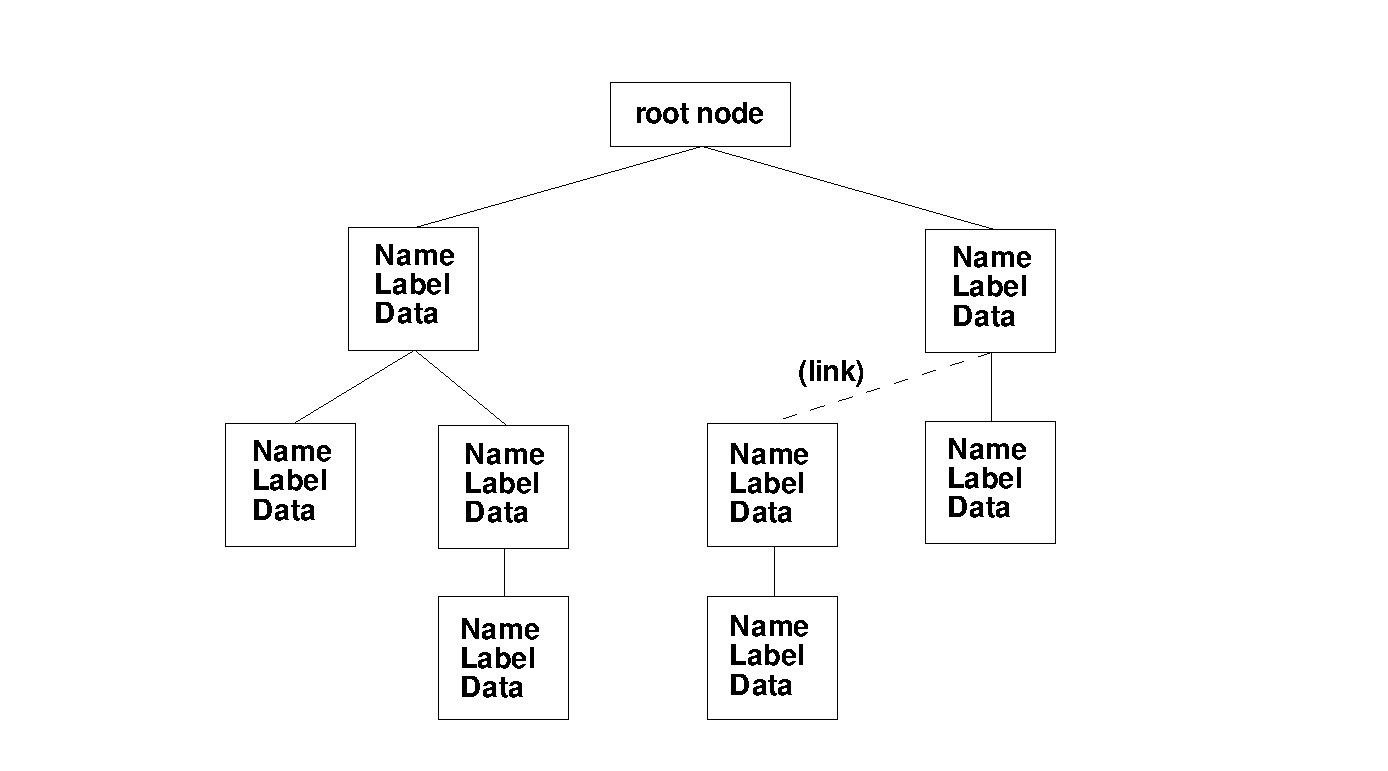
\includegraphics[width=150mm]{figures/intro}}}
\caption{Example CGNS tree-like structure.}
\label{FIGintro}
\end{figure}
%

In order for any user to be able to interpret a CGNS file, its
nodes must be assembled according to particular rules.
For example, Fig.~\ref{FIGintro_2} shows a simple example
of a tree-like structure that organizes some animals into
categories according to rules that most of us are very
familiar with.  (Note that this figure is different from 
Fig.~\ref{FIGintro} in that no ``Labels'' or ``Data'' are
used, only ``Names.'')  The categories 
get narrower and narrower in their scope
as you traverse lower in the tree.  The broadest category here
is ``Animals,'' and the tree narrows all the way down to
particular dogs (two ``Fido''s, a ``Spot,'' and a ``Ginger'').
Knowing ahead of time how this tree is organized allows you
to quickly and easily access whatever particular information
from the tree that you may be interested in.
If someone else were to organize these same animals in a completely
different way, according to different rules, then it would be
difficult for you to access the desired information without
spending a lot of time searching and studying the tree.

% Figure
\begin{figure}[hpbt]
\centerline{{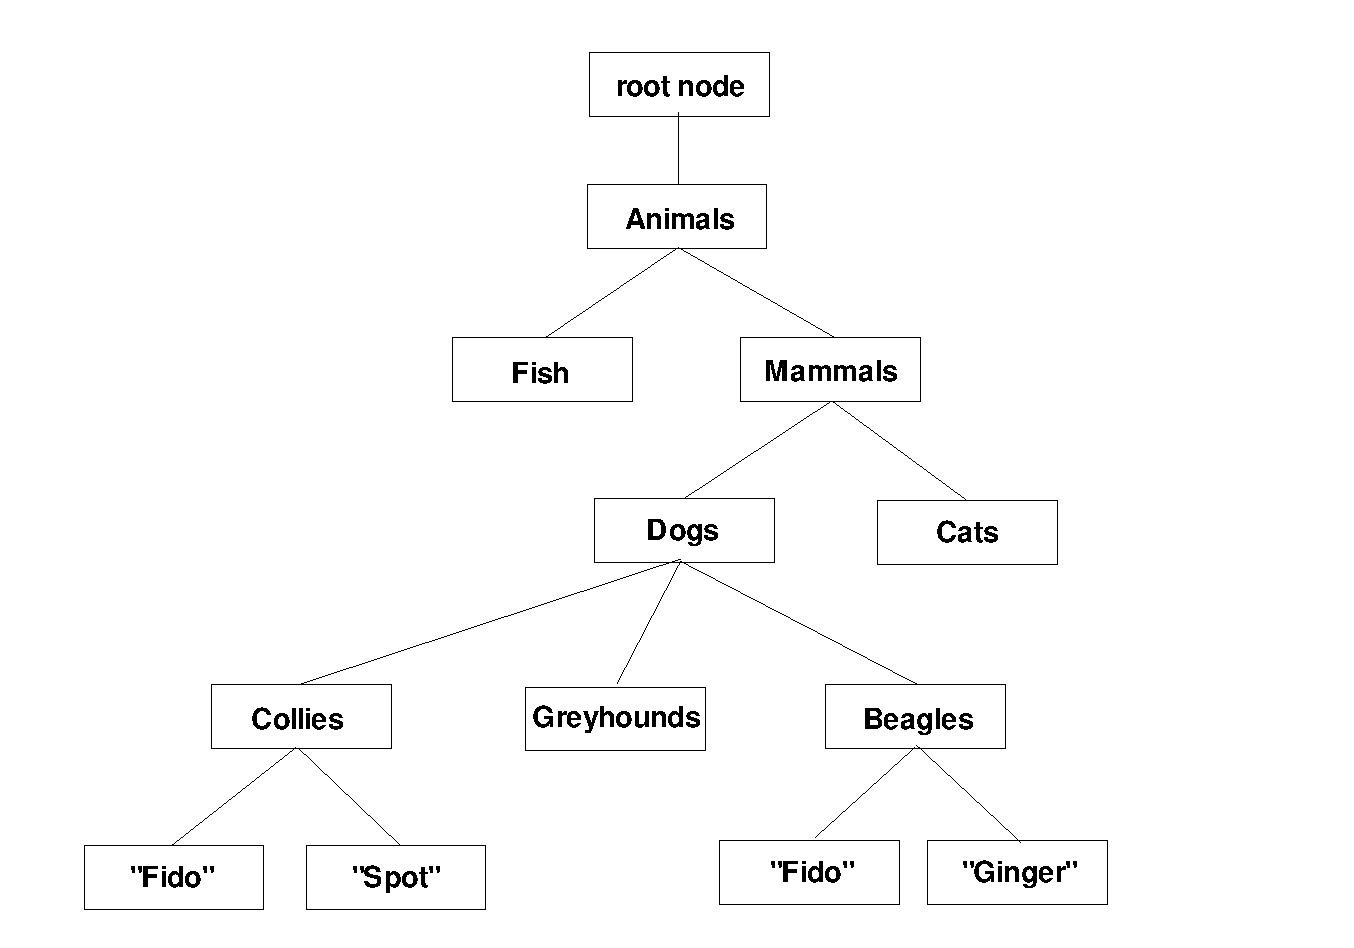
\includegraphics[width=150mm]{figures/intro_2}}}
\caption{Simple tree-like structure that categorizes some animals.}
\label{FIGintro_2}
\end{figure}
%

The particular rules for organizing CGNS files for aerodynamic
data, which allow users to easily access desired information, are described
in the Standard Interface Data Structures (SIDS) 
document \cite{ALLMARAS}.
Because CGNS files are binary files, they cannot be viewed by
the user with standard UNIX ASCII-editing tools.
The utility \underbar{adfviewer} was created to allow users to easily view
CGNS files.

\subsection{How this User's Guide is Organized}

The main content in this User's Guide is located in 
section~\ref{sec:start}, where several simple examples are
given for both structured and unstructured grids.  This section
covers the basics that most users want or need to learn in order
to get started using CGNS.  It is recommended that
the section on structured grids be read first, in its entirety,
even if the user is only interested in unstructured grid
applications.
Some additional information is covered
in section~\ref{sec:advanced}; these issues are felt to be important
(i.e., most users will want to eventually include them), but
they are not as crucial as the basic items covered in 
section~\ref{sec:start}.  Finally, sections~\ref{sec:trouble} and
\ref{sec:FAQ} briefly cover troubleshooting and frequently asked
questions, respectively.  

Note that all of the codes and code segments given in this document are
available as complete codes from the CGNS site at SourceForge
(\underbar{sourceforge.net/projects/cgns}).
The names of these codes and their functions are listed in
Appendix~\ref{sec:codes}.  Also note that not all CGNS capabilities
are covered in this document.  It is meant to be a fairly simple
introductory guide only. 

\newpage
\section{GETTING STARTED} \label{sec:start}

The rules and conventions governing how the nodes in a CGNS 
file are organized, including their names and labels, are 
specified in the SIDS
document \cite{ALLMARAS}, with additional details in 
\cite{CGNS1} \cite{CGNS2}.
These documents also specify in detail how CFD information
is to be stored within the nodes in a standardized fashion so that 
other users can easily access and read it.
When a CGNS file strictly adheres to the rules given in
the SIDS document, it is said to be
``SIDS-compliant.''  A CGNS file must be SIDS-compliant in
order for other users to be able to properly interpret it.
A brief overview of the most commonly used aspects of the SIDS is given 
in Appendix~\ref{sec:sidsoverview}.

However, to get started with CGNS, it is not necessary
for the user to fully understand the SIDS document or Appendix~\ref{sec:sidsoverview}.  
The mid-level, or API calls have been created to aid users
in writing and reading CGNS files that are SIDS-compliant.  
\footnote{There are currently two levels of programming access to CGNS.
The lowest level consists of ADF- or HDF5-level calls.  These calls
perform the most basic functions, such as creating a child node,
writing data, reading data, etc.
However, these low-level calls know nothing at all about the SIDS,
so the user is responsible for putting data in the correct 
place, to make the CGNS file SIDS-compliant.
The mid-level, or API calls, which always begin with the characters
``cg\_'', were written with knowledge of the SIDS.
Therefore, it is easier to adhere to the SIDS standards when
writing a CGNS file using the API calls, and some checks for
SIDS-compliance are also made by the API calls when accessing a CGNS file
(SIDS compliance is not guaranteed, but the API calls
go a long way toward facilitating it).  The API calls also
drastically shorten the calling sequences necessary to perform
many of the functions needed to create and read CGNS files.}
Using the API, most CFD data of interest to the majority of users can be
written into or read from a CGNS file very easily with only an
elementary understanding of the SIDS.

%CFD programmers may find it useful to create their own
%high-level routines when they implement CGNS.  By ``high-level,''
%we mean routines that are specific to the user's particular
%application.  For example, the SIDS allows for the storage of many
%different possibilities for data arrays such
%as coordinate variables.  The API,
%therefore, has created a general enough function that the many
%possibilities are allowed.  However, for a given application,
%it may be the case that (for example) CoordinateX, CoordinateY, 
%and CoordinateZ are
%{\it always} output or read in.  Therefore, the user may
%find it convenient to write a single high-level routine
%``putgrid'' that makes use of mid-level
%API functions to write the grid (CoordinateX, CoordinateY,
%and CoordinateZ) as desired.  Similarly, a
%possible high-level routine ``getgrid'' may
%want to first check to make sure the desired variables 
%(CoordinateX, CoordinateY, and CoordinateZ) are available in 
%the CGNS file, and exit the program gracefully if they are not.

In the following sections, we give detailed instructions on
how to create typical CGNS files or portions of files.  These 
instructions are
given in the form of simple examples.  They make use of the 
mid-level API calls, although not all API calls are covered in
this document (a complete list of available API calls can be
found in \cite{POIRIER99}).  We recommend that the user
read through the examples in this section {\it in order}, because some
information in the later sections depends on being
familiar with information given in the earlier ones.  Hopefully, 
users should be able to easily
extend these simple examples to their own applications.
Additional applications are covered in 
section~\ref{sec:advanced}.  For those users already familiar with
the PLOT3D format for CFD data \cite{WALATKA}, we include a detailed description
on reading and writing PLOT3D-type variables in a CGNS file in
Appendix~\ref{sec:plot3d}.

Also note that we have delayed the discussion
of units and nondimensionalization until section~\ref{sec:advanced}.
For now, all examples simply store and retrieve pure {\it numbers},
and it is assumed that the user knows what the dimensions or
nondimensionalizations of each variable are.

\newpage
\subsection{Structured Grid} \label{sec:str}

This first section gives several structured grid examples, whereas
section~\ref{sec:unstr} gives unstructured grid examples.  However,
we recommend that section~\ref{sec:str} be read first, in its entirety,
even if the user is only interested in unstructured grid
applications.  This is because much of the organization of the
CGNS files is identical for both grid types, and later sections
of this document assume that the user is familiar with information
given in earlier sections.

\subsubsection{Single-Zone Structured Grid} \label{sec:singlegrid}

This first example is for a very simple 3-D Cartesian grid of size
$21 \times 17 \times 9$.  The grid points themselves are created
using the following FORTRAN code snippet:

--------------------------------------------------------------------

{\tt \indent         do k=1,nk
\newline\indent\indent           do j=1,nj
\newline\indent\indent\indent             do i=1,ni
\newline\indent\indent\indent\indent               x(i,j,k)=float(i-1)
\newline\indent\indent\indent\indent               y(i,j,k)=float(j-1)
\newline\indent\indent\indent\indent               z(i,j,k)=float(k-1)
\newline\indent\indent\indent             enddo
\newline\indent\indent           enddo
\newline\indent         enddo}

--------------------------------------------------------------------

\noindent where {\tt ni=21}, {\tt nj=17}, and {\tt nk=9}.  
A picture of the grid is shown in
Fig.~\ref{FIGgrid_cartesian}.

% Figure
\begin{figure}[hpbt]
\centerline{{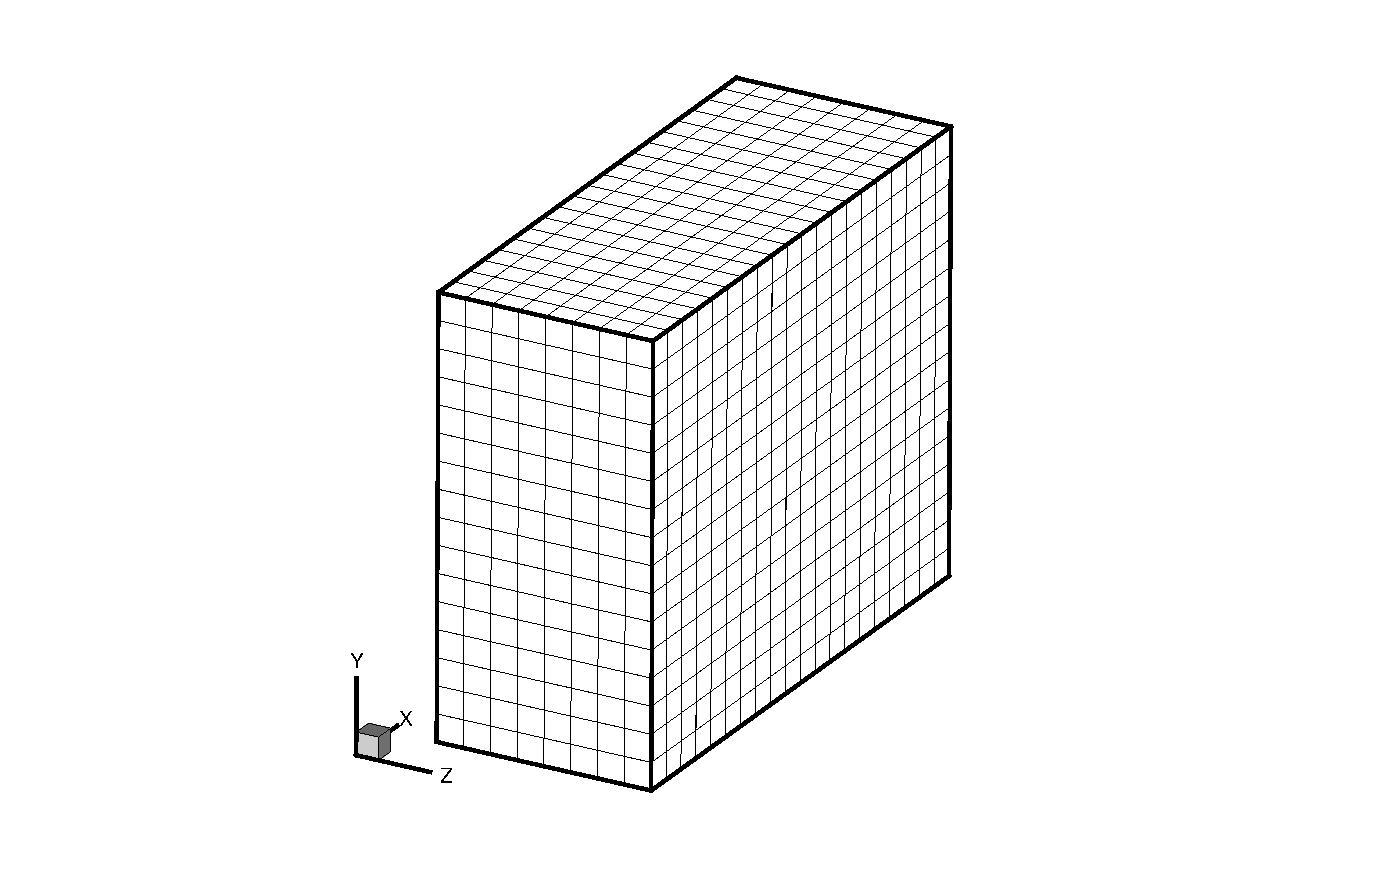
\includegraphics[width=120mm]{figures/grid_cartesian}}}
\caption{Simple Cartesian structured grid.}
\label{FIGgrid_cartesian}
\end{figure}
%

A complete FORTRAN code that creates this grid and
uses API calls to write it
to a CGNS file called {\tt grid.cgns} is shown here 
(note that a FORTRAN line continuation
is denoted by a {\tt +}).  This (and all later) coded examples
are available from the CGNS site at SourceForge
(\underbar{sourceforge.net/projects/cgns}).
See Appendix~\ref{sec:codes}.

--------------------------------------------------------------------

{\tt 
\indent       program write\_grid\_str
\newline c
\newline c   Creates simple 3-D structured grid and writes it to a
\newline c   CGNS file.
\newline c
\newline c   This program uses the fortran convention that all
\newline c   variables beginning with the letters i-n are integers,
\newline c   by default, and all others are real
\newline c
\newline c   cgnslib\_f.h file must be located in directory specified by -I during compile:
\newline\indent      include 'cgnslib\_f.h'
\newline c   dimension statements (note that tri-dimensional arrays
\newline c   x,y,z must be dimensioned exactly as (21,17,N) (N>=9)
\newline c   for this particular case or else they will be written to
\newline c   the CGNS file incorrectly!  Other options are to use 1-D
\newline c   arrays, use dynamic memory, or pass index values to a
\newline c   subroutine and dimension exactly there):
\newline\indent      real*8 x(21,17,9),y(21,17,9),z(21,17,9)
\newline\indent      dimension isize(3,3)
\newline\indent      character basename*32,zonename*32
\newline c
\newline c   create gridpoints for simple example:
\newline\indent      ni=21
\newline\indent      nj=17
\newline\indent      nk=9
\newline\indent      do k=1,nk
\newline\indent\indent        do j=1,nj
\newline\indent\indent\indent          do i=1,ni
\newline\indent\indent\indent\indent            x(i,j,k)=float(i-1)
\newline\indent\indent\indent\indent            y(i,j,k)=float(j-1)
\newline\indent\indent\indent\indent            z(i,j,k)=float(k-1)
\newline\indent\indent\indent          enddo
\newline\indent\indent        enddo
\newline\indent      enddo
\newline\indent      write(6,'('' created simple 3-D grid points'')')
\newline c
\newline c  WRITE X, Y, Z GRID POINTS TO CGNS FILE
\newline c  open CGNS file for write
\newline\indent      call cg\_open\_f('grid.cgns',MODE\_WRITE,index\_file,ier)
\newline c  create base (user can give any name)
\newline\indent      basename='Base'
\newline\indent      icelldim=3
\newline\indent      iphysdim=3
\newline\indent      call cg\_base\_write\_f(index\_file,basename,icelldim,iphysdim,
\newline + \indent index\_base,ier)
\newline c  define zone name (user can give any name)
\newline\indent      zonename = 'Zone~~1'
\newline c  vertex size
\newline\indent      isize(1,1)=21
\newline\indent      isize(2,1)=17
\newline\indent      isize(3,1)=9
\newline c  cell size
\newline\indent      isize(1,2)=isize(1,1)-1
\newline\indent      isize(2,2)=isize(2,1)-1
\newline\indent      isize(3,2)=isize(3,1)-1
\newline c  boundary vertex size (always zero for structured grids)
\newline\indent      isize(1,3)=0
\newline\indent      isize(2,3)=0
\newline\indent      isize(3,3)=0
\newline c  create zone
\newline\indent      call cg\_zone\_write\_f(index\_file,index\_base,zonename,isize,
\newline + \indent Structured,index\_zone,ier)
\newline c  write grid coordinates (user must use SIDS-standard names here)
\newline\indent      call cg\_coord\_write\_f(index\_file,index\_base,index\_zone,RealDouble,
\newline + \indent 'CoordinateX',x,index\_coord,ier)
\newline\indent      call cg\_coord\_write\_f(index\_file,index\_base,index\_zone,RealDouble,
\newline + \indent 'CoordinateY',y,index\_coord,ier)
\newline\indent      call cg\_coord\_write\_f(index\_file,index\_base,index\_zone,RealDouble,
\newline + \indent 'CoordinateZ',z,index\_coord,ier)
\newline c  close CGNS file
\newline\indent      call cg\_close\_f(index\_file,ier)
\newline\indent      write(6,'('' Successfully wrote grid to file grid.cgns'')')
\newline\indent      stop
\newline\indent      end
}

--------------------------------------------------------------------

\noindent There are several items to note regarding this
code.  Whenever a new entity is created using the API,
an integer index is returned.  This index is used in subsequent
API calls to refer to the entity.  For example, the above call to
{\tt cg\_open\_f}, which opens the file grid.cgns, assigns to this
entity the index {\tt index\_file}.  This same {\tt index\_file}
is used to identify this entity in subsequent calls.
Similarly, {\tt cg\_base\_write\_f} assigns an index {\tt index\_base} to
the base, {\tt cg\_zone\_write\_f} 
assigns an index {\tt index\_zone} to the zone, and
{\tt cg\_coord\_write\_f} assigns an index {\tt index\_coord}
to each coordinate.

For FORTRAN code, an include statement
pointing to {\tt cgnslib\_f.h} must be present.  (The cgnslib\_f.h
file comes with the CGNS software.)  Also, it is
imperative that the {\tt x}, {\tt y}, and {\tt z} arrays be dimensioned
{\it exactly} as (21,17,$N$), where $N \geq 9$ (or
else as a one-dimensional array of at least size $21*17*9$) 
for this particular example; 
this is because the {\tt cg\_coord\_write\_f}
routine writes the first $21*17*9$ values contained in the
array {\it as it is stored
in memory}.  If {\tt x}, {\tt y}, and {\tt z} are tri-dimensional arrays
and the first two indices 
are dimensioned larger than 21 and 17, respectively, then incorrect
values will be placed in the CGNS file.  In a real
working code, one would probably either (a) use one-dimensional
arrays, (b) dynamically allocate
appropriate memory for {\tt x}, {\tt y}, and {\tt z}, or else (c) pass the index
values to a subroutine and write via an appropriately dimensioned
work array.

In this case, the cell dimension ({\tt icelldim}) is 3
(because the grid is made up of volume cells), and the
physical dimension ({\tt iphysdim}) is 3 (because 3 coordinates
define 3-D).  (Refer to Appendix~\ref{sec:sidsoverview} for a more
detailed description.)  The {\tt isize} array
contains the vertex size, cell size, and
boundary vertex size for each index direction.  For a 3-D
structured grid, the index dimension is always the same as
the cell dimension, so this
means there are 3 vertex sizes, 3 cell sizes, and 3 boundary vertex sizes
(one each for the $i$, $j$, and $k$ directions).  For structured grids, 
the cell size is always one less than the corresponding vertex
size, and the boundary vertex size has no meaning and is always zero.
When writing the grid coordinates, the user must use SIDS-standard
names.  For example, {\tt x}, {\tt y}, and {\tt z} coordinates must be named
{\tt CoordinateX}, {\tt CoordinateY}, and {\tt CoordinateZ},
respectively.  Other standard names exist for other possible choices
(see \cite{ALLMARAS}).
Finally, {\tt basename} and {\tt zonename} must be declared as character
strings, and the integer array {\tt isize} must be dimensioned
appropriately.

The grid coordinate arrays can be written in single or double
precision.  The desired data type is communicated to the API using the
keywords {\tt RealSingle} or {\tt RealDouble}.  The user must
insure that the data type transmitted to the API is consistent with
the the one used in declaring the coordinates arrays.
When it is compiled, the code must also link to the 
compiled CGNS library {\tt libcgns.a}.
Instructions for compiling the CGNS library
are given in README files that come with the CGNS software.

A complete code written in C that performs the same task of
creating grid coordinates and writing them to a CGNS file is given here.

--------------------------------------------------------------------

{\tt
\noindent /*
\newline Creates simple 3-D structured grid and writes it to a
\newline CGNS file.

\noindent UNIX compilation (IRIX 5.3 or higher with mips4\_64 option)
\newline for this program is:
\newline cc -r8 -64 write\_grid\_str.c CGNSLib/lib/libcgns.mips4\_64.a
\newline (CGNSLib/lib/ is the location where the compiled
\newline library libcgns.mips4\_64.a is located)
\newline (Note it is compiled double precision because RealDouble
\newline is used below)
\newline */

\noindent \#include <string.h>
\newline /* must include path to cgnslib.h file: */
\newline \#include "cgnslib.h"

\noindent main()
\newline \{
\newline /*
\newline\indent   dimension statements (note that tri-dimensional arrays
\newline\indent   x,y,z must be dimensioned exactly as [N][17][21] (N>=9)
\newline\indent   for this particular case or else they will be written to
\newline\indent   the CGNS file incorrectly!  Other options are to use 1-D
\newline\indent   arrays, use dynamic memory, or pass index values to a
\newline\indent   subroutine and dimension exactly there):
\newline */
\newline\indent   double x[9][17][21],y[9][17][21],z[9][17][21];
\newline\indent   int isize[3][3];
\newline\indent   int ni,nj,nk,i,j,k;
\newline\indent   int index\_file,icelldim,iphysdim,index\_base;
\newline\indent   int index\_zone,index\_coord;
\newline\indent   char basename[33],zonename[33];

\noindent /* create gridpoints for simple example: */
\newline\indent  ni=21;
\newline\indent  nj=17;
\newline\indent  nk=9;
\newline\indent  for (k=0; k $<$ nk; ++k)
\newline\indent  \{
\newline\indent\indent     for (j=0; j $<$ nj; ++j)
\newline\indent\indent     \{
\newline\indent\indent\indent        for (i=0; i $<$ ni; ++i)
\newline\indent\indent\indent        \{
\newline\indent\indent\indent\indent           x[k][j][i]=i;
\newline\indent\indent\indent\indent           y[k][j][i]=j;
\newline\indent\indent\indent\indent           z[k][j][i]=k;
\newline\indent\indent\indent        \}
\newline\indent\indent     \}
\newline\indent  \}
\newline\indent printf("\texttt{\symbol{92}}ncreated simple 3-D grid points");

\noindent /*  WRITE X, Y, Z GRID POINTS TO CGNS FILE  */
\newline /*  open CGNS file for write  */
\newline\indent  cg\_open("grid\_c.cgns",MODE\_WRITE,\&index\_file);
\newline /*  create base (user can give any name)  */
\newline\indent  strcpy(basename,"Base");
\newline\indent  icelldim=3;
\newline\indent  iphysdim=3;
\newline\indent  cg\_base\_write(index\_file,basename,icelldim,iphysdim,\&index\_base);
\newline /*  define zone name (user can give any name)  */
\newline\indent  strcpy(zonename,"Zone  1");
\newline /*  vertex size  */
\newline\indent  isize[0][0]=21;
\newline\indent  isize[0][1]=17;
\newline\indent  isize[0][2]=9;
\newline /*  cell size  */
\newline\indent  isize[1][0]=isize[0][0]-1;
\newline\indent  isize[1][1]=isize[0][1]-1;
\newline\indent  isize[1][2]=isize[0][2]-1;
\newline /*  boundary vertex size (always zero for structured grids)  */
\newline\indent  isize[2][0]=0;
\newline\indent  isize[2][1]=0;
\newline\indent  isize[2][2]=0;
\newline /*  create zone  */
\newline\indent  cg\_zone\_write(index\_file,index\_base,zonename,*isize,Structured,
\newline \indent \indent \&index\_zone);
\newline /*  write grid coordinates (user must use SIDS-standard names here)  */
\newline\indent  cg\_coord\_write(index\_file,index\_base,index\_zone,RealDouble,"CoordinateX",
\newline \indent \indent x,\&index\_coord);
\newline\indent  cg\_coord\_write(index\_file,index\_base,index\_zone,RealDouble,"CoordinateY",
\newline \indent \indent y,\&index\_coord);
\newline\indent  cg\_coord\_write(index\_file,index\_base,index\_zone,RealDouble,"CoordinateZ",
\newline \indent \indent z,\&index\_coord);
\newline /*  close CGNS file  */
\newline\indent  cg\_close(index\_file);
\newline\indent printf("\texttt{\symbol{92}}nSuccessfully wrote grid to file grid\_c.cgns\texttt{\symbol{92}}n");
\newline\}
}

--------------------------------------------------------------------

\noindent Note that in the C-code, the ``.h'' file that must be included
is called {\tt cgnslib.h}.  From now on, all codes will be given in
FORTRAN only.  The C-equivalent calls are similar, as demonstrated
above.  Also, from now on, complete code will not be shown, but
rather only code segments, in order to save space.  However, complete
codes can be accessed from the CGNS site at SourceForge
(\underbar{sourceforge.net/projects/cgns}).

The CGNS file {\tt grid.cgns} that is created by the code above
is a binary
file that, internally, possesses the tree-like structure
shown in Fig.~\ref{FIGtree_cartesian}.  As mentioned in the
Introduction, each node has a name, a label, and may or
may not contain data.  In the example in the figure, all the
nodes contain data except for the {\tt GridCoordinates} node,
for which {\tt MT} indicates no data.

% Figure
\begin{figure}[hpbt]
\centerline{{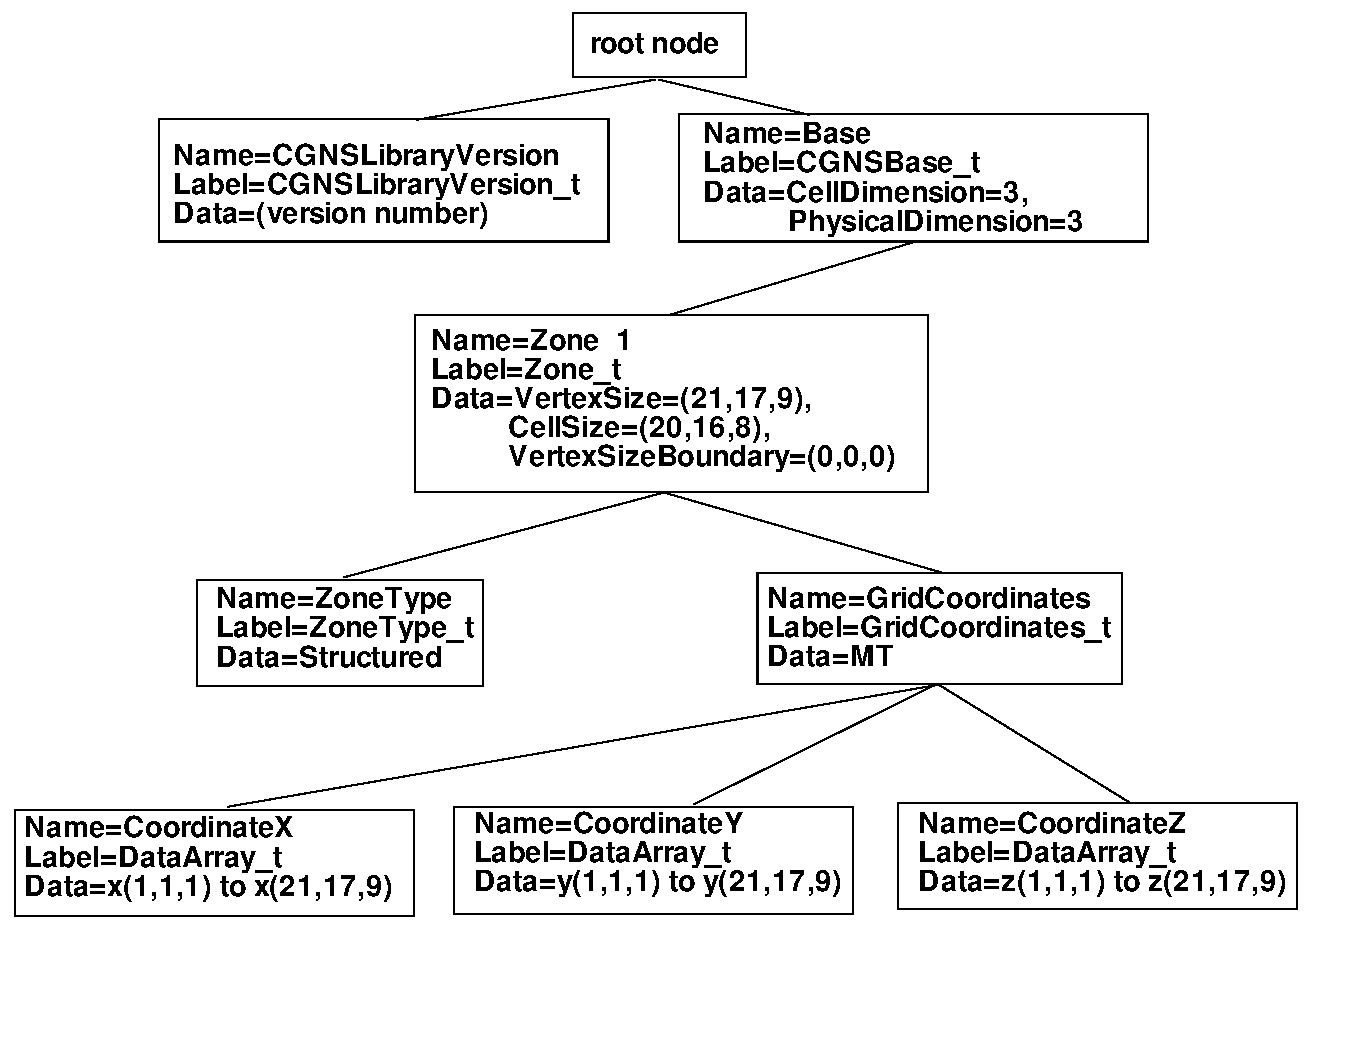
\includegraphics[width=150mm]{figures/tree_cartesian}}}
\caption{Layout of CGNS file for simple Cartesian 
structured grid.}
\label{FIGtree_cartesian}
\end{figure}
%

However, the user really does not need to know the full details of
the tree-like structure in this case.  The API has automatically
created a SIDS-compliant CGNS file!  Now, the user can
just as easily read the CGNS file using the API.
The FORTRAN code segment used to read the CGNS file
{\tt grid.cgns} that we just created is given here:

--------------------------------------------------------------------

{\tt \noindent c  READ X, Y, Z GRID POINTS FROM CGNS FILE
\newline\indent      include 'cgnslib\_f.h'
\newline c   open CGNS file for read
\newline\indent      call cg\_open\_f('grid.cgns',MODE\_READ,index\_file,ier)
\newline c  we know there is only one base (real working code would check!)
\newline\indent      index\_base=1
\newline c  we know there is only one zone (real working code would check!)
\newline\indent      index\_zone=1
\newline c   get zone size (and name - although not needed here)
\newline\indent      call cg\_zone\_read\_f(index\_file,index\_base,index\_zone,zonename,
\newline + \indent isize,ier)
\newline c   lower range index 
\newline\indent      irmin(1)=1
\newline\indent      irmin(2)=1
\newline\indent      irmin(3)=1
\newline c   upper range index of vertices
\newline\indent      irmax(1)=isize(1,1)
\newline\indent      irmax(2)=isize(2,1)
\newline\indent      irmax(3)=isize(3,1)
\newline c   read grid coordinates
\newline\indent      call cg\_coord\_read\_f(index\_file,index\_base,index\_zone,
\newline + \indent 'CoordinateX',RealSingle,irmin,irmax,x,ier)
\newline\indent      call cg\_coord\_read\_f(index\_file,index\_base,index\_zone,
\newline + \indent 'CoordinateY',RealSingle,irmin,irmax,y,ier)
\newline\indent      call cg\_coord\_read\_f(index\_file,index\_base,index\_zone,
\newline + \indent 'CoordinateZ',RealSingle,irmin,irmax,z,ier)
\newline c  close CGNS file
\newline\indent      call cg\_close\_f(index\_file,ier)}

--------------------------------------------------------------------

\noindent Note that this
FORTRAN coding is very rudimentary.  It
assumes that we know that there is only one base and one zone.
In a real working code, one
should check the numbers in the file, and either
allow for the possibility of multiple bases or zones,
or explicitly disallow it.  Also, this coding implicitly 
assumes that the {\tt grid.cgns} file is a 3-D structured grid
(cell dimension = physical dimension = 3).  In a real working
code, one should check to make sure that this is true, or
else allow for other possibilities.  One
should also check to make sure the zone type is {\tt Structured}
if this is the type expected.

As before, the {\tt x}, {\tt y}, and {\tt z} arrays in this case {\it must}
be dimensioned correctly:  for a tri-dimensional array,
(21,17,$N$), where $N \geq 9$.
(In a real
working code, one would probably either (a) use one-dimensional
arrays, (b) dynamically allocate
appropriate memory for {\tt x}, {\tt y}, and {\tt z} after reading isize, 
or else (c) pass the isize
values to a subroutine and dimension a work array appropriately
prior to reading.)
Also note that, regardless of the precision in which the
grid coordinates were written
to the CGNS file (single or double), one can read them 
either way; the API automatically
performs the translation.  (The arrays {\tt x}, {\tt y}, and {\tt z} in the code above
must be declared
as single precision if {\tt RealSingle} is used and as
double precision if {\tt RealDouble} is used.)
Finally, {\tt isize} should be dimensioned appropriately,
{\tt zonename} should be declared as a character variable,
and {\tt irmin} and {\tt irmax} should be dimensioned appropriately.

\subsubsection{Single-Zone Structured Grid and Flow Solution} \label{sec:flowsoln}

In this section, we now write a flow solution associated with
the grid from section~\ref{sec:singlegrid}.  We assume that
we have two flow solution arrays available:  static density and 
static pressure.  To illustrate three important options, we will
show how to write the flow solution (a) at vertices, (b) at
cell centers, and (c) at cell centers plus rind cells.  

~

\noindent\underbar{(a) Flow Solution at Vertices}

The first option is illustrated schematically in 2-D in 
Fig.~\ref{FIGvertex}.  Simply stated, a {\tt Vertex} flow solution is located at the
same location as the grid points.  Assuming that the
grid points have already been written to a CGNS file, the
following FORTRAN code segment adds the flow solution at
vertices:

% Figure
\begin{figure}[hpbt]
\centerline{{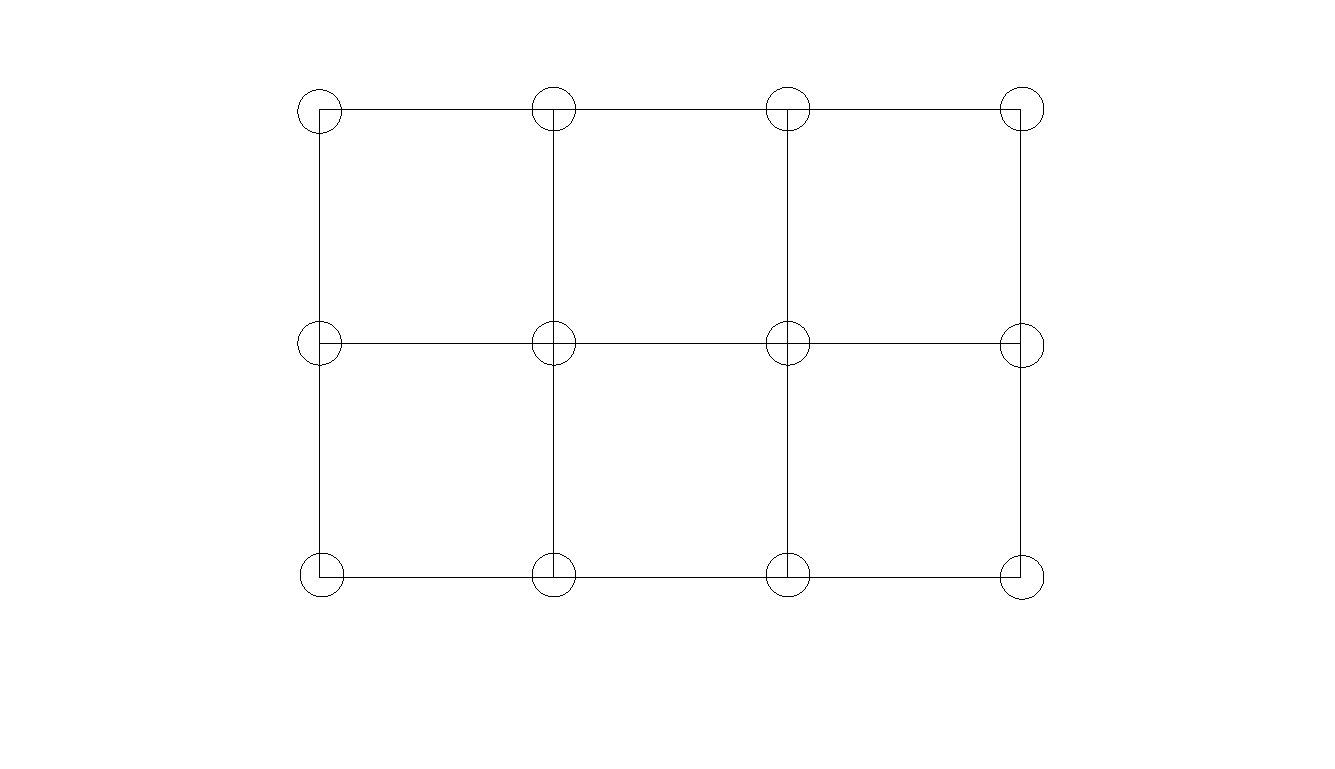
\includegraphics[width=120mm]{figures/vertex}}}
\caption{Schematic showing location (circles) of {\tt Vertex} 
flow solution relative to grid.}
\label{FIGvertex}
\end{figure}
%

--------------------------------------------------------------------

{\tt \noindent c  WRITE FLOW SOLUTION TO EXISTING CGNS FILE
\newline\indent      include 'cgnslib\_f.h'
\newline c  open CGNS file for modify
\newline\indent      call cg\_open\_f('grid.cgns',MODE\_MODIFY,index\_file,ier)
\newline c  we know there is only one base (real working code would check!)
\newline\indent      index\_base=1
\newline c  we know there is only one zone (real working code would check!)
\newline\indent      index\_zone=1
\newline c  define flow solution node name (user can give any name)
\newline\indent      solname = 'FlowSolution'
\newline c  create flow solution node
\newline\indent      call cg\_sol\_write\_f(index\_file,index\_base,index\_zone,solname,
\newline + \indent Vertex,index\_flow,ier)
\newline c  write flow solution (user must use SIDS-standard names here)
\newline\indent      call cg\_field\_write\_f(index\_file,index\_base,index\_zone,index\_flow,
\newline + \indent RealDouble,'Density',r,index\_field,ier)
\newline\indent      call cg\_field\_write\_f(index\_file,index\_base,index\_zone,index\_flow,
\newline + \indent RealDouble,'Pressure',p,index\_field,ier)
\newline c  close CGNS file
\newline\indent      call cg\_close\_f(index\_file,ier)}

--------------------------------------------------------------------

In this code, the density ({\tt r}) and pressure
({\tt p}) variables {\it must} be dimensioned
correctly for this particular case:  for a tri-dimensional array,
(21,17,$N$), where $N \geq 9$
(see discussion in section~\ref{sec:singlegrid}).  
Note that the API, knowing that the flow solution type is 
{\tt Vertex}, automatically writes out the correct index
range, corresponding with the zone's grid index range.
Also note that we opened the existing CGNS file and modified it 
({\tt MODE\_MODIFY}) - we
knew ahead of time that only one base and only one zone exist;
a real working code would make appropriate checks.  Finally,
{\tt solname} should be declared as a character variable and
{\tt r} and {\tt p} must be declared as double precision variables when
{\tt RealDouble} type is used.

The layout of the CGNS file with the flow 
solution at vertices included 
is shown in Fig.~\ref{FIGtree_cartesian_solV}.
The three nodes under {\tt GridCoordinates\_t} have been left out
to conserve space in the figure,
but they exist as indicated by the three unconnected lines.

% Figure
\begin{figure}[hpbt]
\centerline{{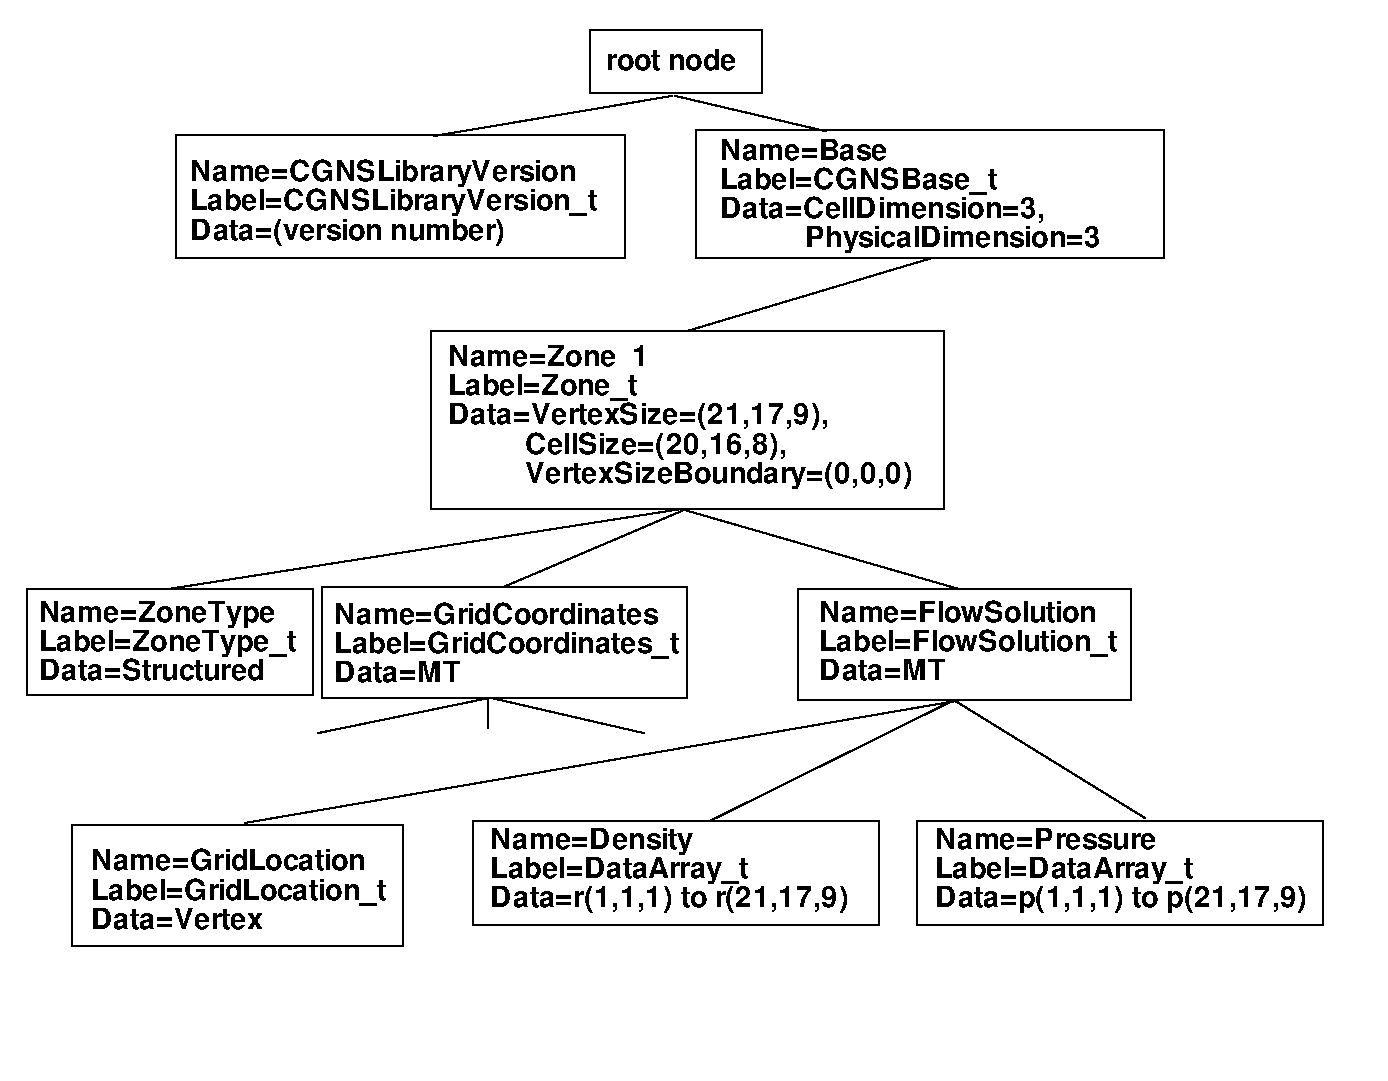
\includegraphics[width=150mm]{figures/tree_cartesian_solV}}}
\caption{Layout of CGNS file for simple Cartesian
structured grid with flow solution at vertices.  (Note: because
{\tt GridLocation} = {\tt Vertex} is the default, it is not
necessary to specify it.)}
\label{FIGtree_cartesian_solV}
\end{figure}
%

The vertex flow solution can be read in using the following 
FORTRAN code segment (can read in as single or double precision -- see
discussion in section~\ref{sec:singlegrid}):

--------------------------------------------------------------------

{\tt \noindent c  READ FLOW SOLUTION FROM CGNS FILE
\newline\indent      include 'cgnslib\_f.h'
\newline c  open CGNS file for read
\newline\indent      call cg\_open\_f('grid.cgns',MODE\_READ,index\_file,ier)
\newline c  we know there is only one base (real working code would check!)
\newline\indent      index\_base=1
\newline c  we know there is only one zone (real working code would check!)
\newline\indent      index\_zone=1
\newline c  we know there is only one FlowSolution\_t (real working code would check!)
\newline\indent      index\_flow=1
\newline c   get zone size (and name - although not needed here)
\newline\indent      call cg\_zone\_read\_f(index\_file,index\_base,index\_zone,zonename,
\newline + \indent isize,ier)
\newline c   lower range index
\newline\indent      irmin(1)=1
\newline\indent      irmin(2)=1
\newline\indent      irmin(3)=1
\newline c   upper range index - use vertex dimensions
\newline c   checking GridLocation first (real working code would check
\newline c   to make sure there are no Rind cells also!):
\newline\indent      call cg\_sol\_info\_f(index\_file,index\_base,index\_zone,index\_flow,
\newline + \indent solname,loc,ier)
\newline\indent      if (loc .ne. Vertex) then
\newline\indent\indent        write(6,'('' Error, GridLocation must be Vertex!'')')
\newline\indent\indent        stop
\newline\indent      end if
\newline\indent      irmax(1)=isize(1,1)
\newline\indent      irmax(2)=isize(2,1)
\newline\indent      irmax(3)=isize(3,1)
\newline c   read flow solution
\newline\indent      call cg\_field\_read\_f(index\_file,index\_base,index\_zone,index\_flow,
\newline + \indent 'Density',RealSingle,irmin,irmax,r,ier)
\newline\indent      call cg\_field\_read\_f(index\_file,index\_base,index\_zone,index\_flow,
\newline + \indent 'Pressure',RealSingle,irmin,irmax,p,ier)
\newline c  close CGNS file
\newline\indent      call cg\_close\_f(index\_file,ier)}

--------------------------------------------------------------------

\noindent Note that this code segment assumes that it is known that
the flow solution contains no rind data (to be covered in detail
below).  If rind data {\it does} exist, but the user does not
account for it, then the flow solution information will be read
incorrectly.  Hence, a real working code would check for rind
cells, and adjust the dimensions and index ranges appropriately.
Other similar cautions as those mentioned earlier regarding
dimensioning of variables, real working code checks, etc.,
apply here as well.  These cautions will not always be repeated from
this point forward.

~

\noindent\underbar{(b) Flow Solution at Cell Centers}

The option for outputting the flow solution at cell centers
is illustrated schematically in 2-D in
Fig.~\ref{FIGcellcenter}.  The flow solutions are defined at
the {\it centers} of the cells defined by the 
four surrounding grid points.  In 3-D,
the cell centers are defined by eight surrounding grid points.
The code segment to write to cell centers is identical to that given
above for vertices, except that the call to
{\tt cg\_sol\_write\_f} is replaced by:

% Figure
\begin{figure}[hpbt]
\centerline{{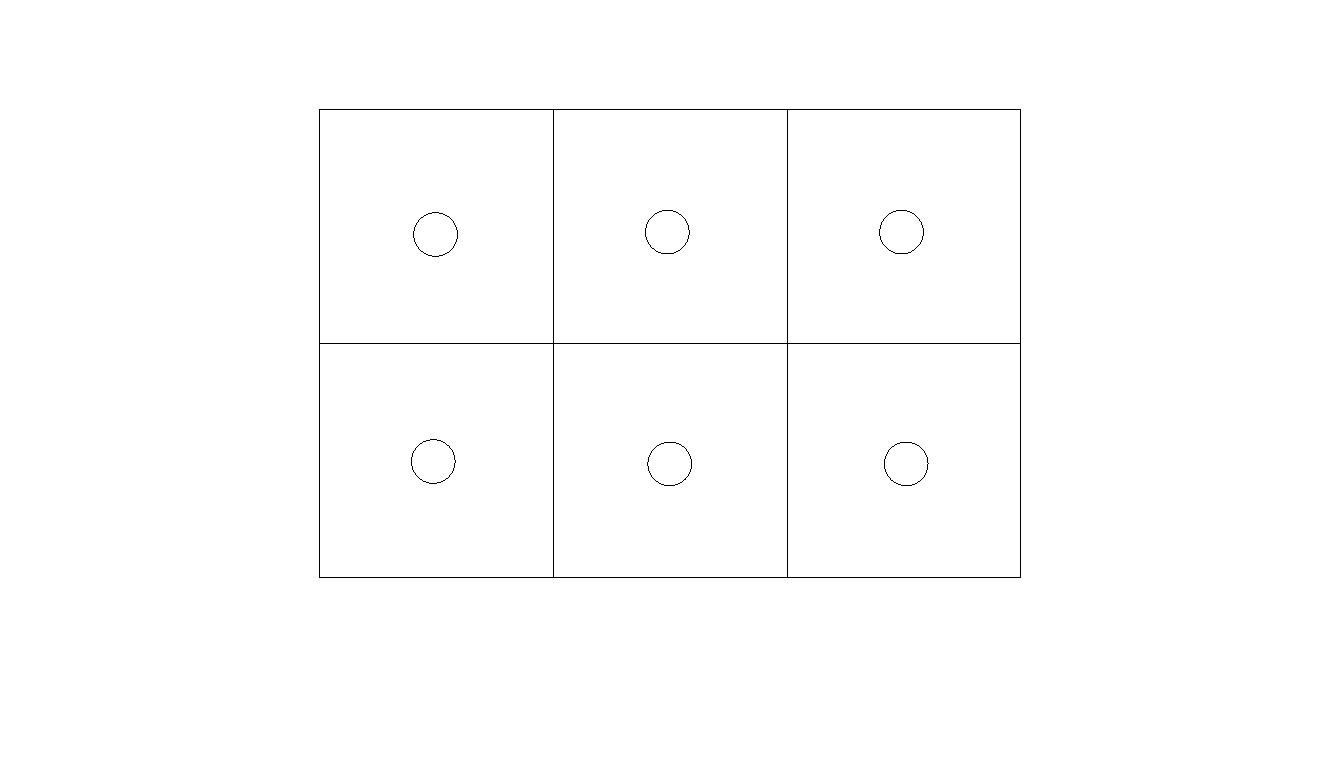
\includegraphics[width=120mm]{figures/cellcenter}}}
\caption{Schematic showing location (circles) of {\tt CellCenter}
flow solution relative to grid.}
\label{FIGcellcenter}
\end{figure}
%

--------------------------------------------------------------------

{\tt \noindent c  create flow solution node (NOTE USE OF CellCenter HERE)
\newline\indent      call cg\_sol\_write\_f(index\_file,index\_base,index\_zone,solname,CellCenter,
\newline + \indent index\_flow,ier)}

--------------------------------------------------------------------

\noindent Also, now the density ({\tt r}) and pressure
({\tt p}) variables must be dimensioned
correctly for this particular case:  for a tri-dimensional array,
(20,16,$N$), where $N \geq 8$
(i.e., one less in each index dimension than the grid itself).
Again, the API, knowing that the flow solution type is
{\tt CellCenter}, automatically writes out the correct index
range, corresponding with the zone's grid index range minus 1 in
each index direction.

The layout of the CGNS file with the flow
solution at cell centers is shown (below the
{\tt FlowSolution\_t} node only) in Fig.~\ref{FIGtree_cartesian_solC}.
Note that the indices over which the flow solutions are written
are now from $(1,1,1)$ to $(20,16,8)$ (contrast with 
the {\tt FlowSolution} part of Fig.~\ref{FIGtree_cartesian_solV}).

% Figure
\begin{figure}[hpbt]
\centerline{{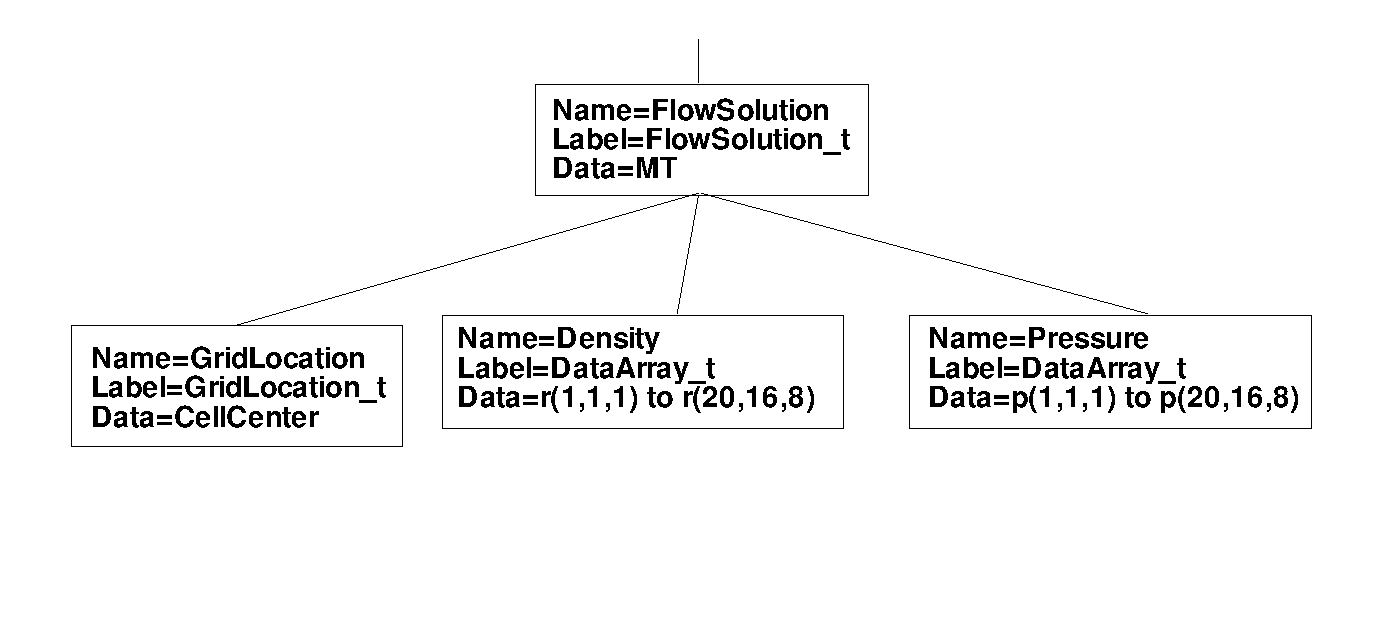
\includegraphics[width=150mm]{figures/tree_cartesian_solC}}}
\caption{Layout of CGNS file (under {\tt FlowSolution\_t} node)
for simple Cartesian structured grid with flow solution at cell
centers.}
\label{FIGtree_cartesian_solC}
\end{figure}
%

The FORTRAN code segment to read in the solution at cell centers
is the same as that given above for vertices, except that the section that
defines {\tt irmax} is replaced by:

--------------------------------------------------------------------

{\tt \noindent c   upper range index - use cell dimensions
\newline c   checking GridLocation first (real working code would check
\newline c   to make sure there are no Rind cells also!):
\newline\indent      call cg\_sol\_info\_f(index\_file,index\_base,index\_zone,index\_flow,
\newline + \indent solname,loc,ier)
\newline\indent      if (loc .ne. CellCenter) then
\newline\indent\indent        write(6,'('' Error, GridLocation must be CellCenter!'')')
\newline\indent\indent        stop
\newline\indent      end if
\newline\indent      irmax(1)=isize(1,2)
\newline\indent      irmax(2)=isize(2,2)
\newline\indent      irmax(3)=isize(3,2)}

--------------------------------------------------------------------

\noindent and, as usual, the {\tt r} and {\tt p} arrays must be dimensioned 
appropriately.

~

\noindent\underbar{(c) Flow Solution at Cell Centers With Additional Rind Data}

Rind data is additional flow solution data {\it exterior} to a
grid, at ``ghost'' locations.  Rind data
can be associated with other {\tt GridLocation} values
beside {\tt CellCenter}, although we only show an example
using {\tt CellCenter} here.
Furthermore, this example is for structured grids only, for which Rind
data can be defined implicitly (via indexing conventions alone).
The option for outputting the flow solution at cell centers
with additional rind data is illustrated schematically in 2-D in
Fig.~\ref{FIGcellcenter_rind}.  In this diagram, we show one layer
of rind cell data in the row below the grid itself.  There could be
rind data at other sides of the grid, or there could be
more than one row at a given side.  

% Figure
\begin{figure}[hpbt]
\centerline{{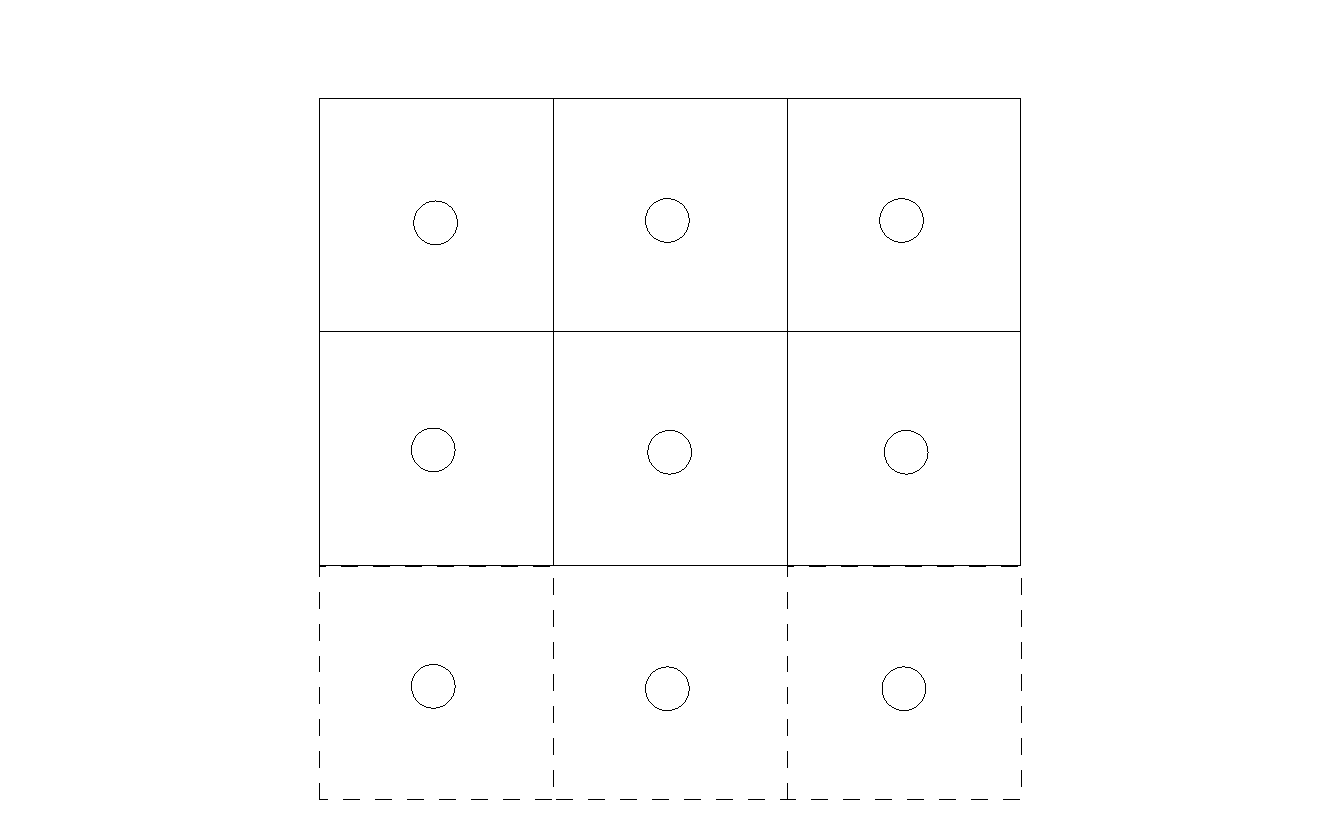
\includegraphics[width=120mm]{figures/cellcenter_rind}}}
\caption{Schematic showing location (circles) of {\tt CellCenter}
flow solution, including rind cells, relative to grid.}
\label{FIGcellcenter_rind}
\end{figure}
%

In CGNS, the flow solution at
rind cells is not stored as separate entities, but rather the 
flow solution range is extended to {\it include} the rind cells.  For
example, in the 2-D schematic of Fig.~\ref{FIGcellcenter_rind}, instead
of an index range of {\tt p(3,2)} for pressures stored at the cell
centers, the flow solution would now have an index range of 
{\tt p(3,0:2)} or {\tt p(3,3)}.  See \cite{ALLMARAS} for details.

For our 3-D example, we assume that we have one row of rind data
at 4 faces of the zone ({\tt ilo, ihi, jlo, jhi}, where these
represent the low and high ends of the {\it i} and {\it j}
directions, respectively), and
no rind cells at {\tt klo} or {\tt khi} (at either end of the {\it k}
direction).
The code segment to write the flow solution and rind data is as
follows:

--------------------------------------------------------------------

{\tt \noindent c  WRITE FLOW SOLUTION TO EXISTING CGNS FILE
\newline\indent      include 'cgnslib\_f.h'
\newline c  open CGNS file for modify
\newline\indent      call cg\_open\_f('grid.cgns',MODE\_MODIFY,index\_file,ier)
\newline c  we know there is only one base (real working code would check!)
\newline\indent      index\_base=1
\newline c  we know there is only one zone (real working code would check!)
\newline\indent      index\_zone=1
\newline c  define flow solution node name (user can give any name)
\newline\indent      solname = 'FlowSolution'
\newline c  create flow solution node
\newline\indent      call cg\_sol\_write\_f(index\_file,index\_base,index\_zone,solname,CellCenter,
\newline + \indent index\_flow,ier)
\newline c  go to position within tree at FlowSolution\_t node
\newline\indent      call cg\_goto\_f(index\_file,index\_base,ier,'Zone\_t',index\_zone,
\newline + \indent 'FlowSolution\_t',index\_flow,'end')
\newline c   write rind information under FlowSolution\_t node (ilo,ihi,jlo,jhi,klo,khi)
\newline\indent      irinddata(1)=1
\newline\indent      irinddata(2)=1
\newline\indent      irinddata(3)=1
\newline\indent      irinddata(4)=1
\newline\indent      irinddata(5)=0
\newline\indent      irinddata(6)=0
\newline\indent      call cg\_rind\_write\_f(irinddata,ier)
\newline c  write flow solution (user must use SIDS-standard names here)
\newline\indent      call cg\_field\_write\_f(index\_file,index\_base,index\_zone,index\_flow,
\newline + \indent RealDouble,'Density',r,index\_field,ier)
\newline\indent      call cg\_field\_write\_f(index\_file,index\_base,index\_zone,index\_flow,
\newline + \indent RealDouble,'Pressure',p,index\_field,ier)
\newline c  close CGNS file
\newline\indent      call cg\_close\_f(index\_file,ier)}

--------------------------------------------------------------------

\noindent Note that in the case of rind data, the user must
position the {\tt Rind\_t} node appropriately, using the
{\tt cg\_goto\_f} call.  In this case, the {\tt Rind\_t} node belongs under
the {\tt FlowSolution\_t} node.

For this case of cell center flow solution
with rind data, the density ({\tt r}) and pressure ({\tt p})
are written to the CGNS file with the following index ranges:
from $i=0$ to $i=20+1=21$ (or a total $i$
length of 22), from $j=0$ to $j=16+1=17$ (or a total $j$
length of 18), and from $k=1$ to $k=8$.  The variables {\tt r} and {\tt p} must
be dimensioned appropriately to reflect these index ranges
modified by the rind values.

The layout of the CGNS file for this example (below the
{\tt FlowSolution\_t} node only) is shown in
Fig.~\ref{FIGtree_cartesian_solCR}.  Compare this figure with
Figs.~\ref{FIGtree_cartesian_solV} and \ref{FIGtree_cartesian_solC}.

% Figure
\begin{figure}[hpbt]
\centerline{{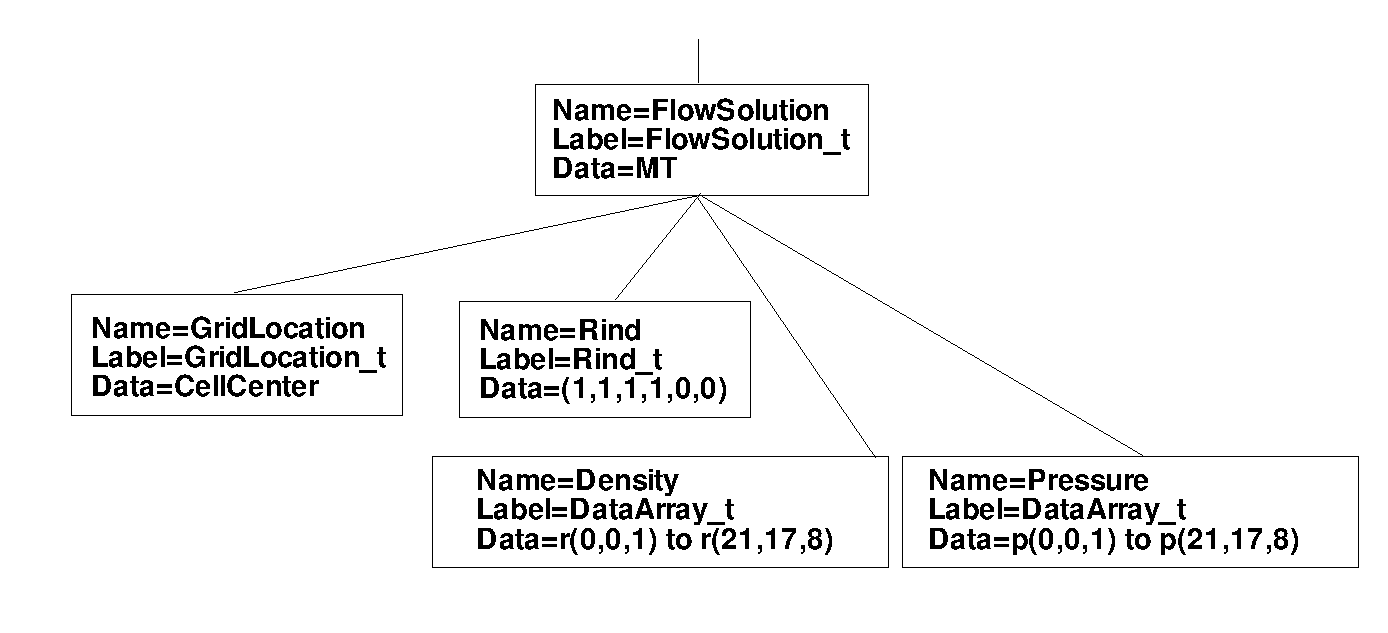
\includegraphics[width=150mm]{figures/tree_cartesian_solCR}}}
\caption{Layout of CGNS file (under {\tt FlowSolution\_t} node)
for simple Cartesian structured grid with flow solution at cell
centers plus rind data.}
\label{FIGtree_cartesian_solCR}
\end{figure}
%

A FORTRAN code segment to read the flow solution for this example is:

--------------------------------------------------------------------

{\tt \noindent c  READ FLOW SOLUTION FROM CGNS FILE
\newline\indent      include 'cgnslib\_f.h'
\newline c  open CGNS file for read
\newline\indent      call cg\_open\_f('grid.cgns',MODE\_READ,index\_file,ier)
\newline c  we know there is only one base (real working code would check!)
\newline\indent      index\_base=1
\newline c  we know there is only one zone (real working code would check!)
\newline\indent      index\_zone=1
\newline c  we know there is only one FlowSolution\_t (real working code would check!)
\newline\indent      index\_flow=1
\newline c   get zone size (and name - although not needed here)
\newline\indent      call cg\_zone\_read\_f(index\_file,index\_base,index\_zone,zonename,isize,ier)
\newline c  go to position within tree at FlowSolution\_t node
\newline\indent      call cg\_goto\_f(index\_file,index\_base,ier,'Zone\_t',index\_zone,
\newline + \indent 'FlowSolution\_t',index\_flow,'end')
\newline c  read rind data
\newline\indent      call cg\_rind\_read\_f(irinddata,ier)
\newline c   lower range index
\newline\indent      irmin(1)=1
\newline\indent      irmin(2)=1
\newline\indent      irmin(3)=1
\newline c   upper range index - use cell dimensions and rind info
\newline c   checking GridLocation first:
\newline\indent      call cg\_sol\_info\_f(index\_file,index\_base,index\_zone,index\_flow,
\newline + \indent     + solname,loc,ier)
\newline\indent      if (loc .ne. CellCenter) then
\newline\indent\indent        write(6,'('' Error, GridLocation must be CellCenter!'')')
\newline\indent\indent        stop
\newline\indent      end if
\newline\indent      irmax(1)=isize(1,2)+irinddata(1)+irinddata(2)
\newline\indent      irmax(2)=isize(2,2)+irinddata(3)+irinddata(4)
\newline\indent      irmax(3)=isize(3,2)+irinddata(5)+irinddata(6)
\newline c   read flow solution
\newline\indent      call cg\_field\_read\_f(index\_file,index\_base,index\_zone,index\_flow,
\newline + \indent 'Density',RealSingle,irmin,irmax,r,ier)
\newline\indent      call cg\_field\_read\_f(index\_file,index\_base,index\_zone,index\_flow,
\newline + \indent 'Pressure',RealSingle,irmin,irmax,p,ier)
\newline c  close CGNS file
\newline\indent      call cg\_close\_f(index\_file,ier)}

--------------------------------------------------------------------

\subsubsection{Single-Zone Structured Grid with Boundary Conditions} \label{sec:bcstruct}

To illustrate the use of boundary conditions, we again use the
same single-zone Cartesian grid from section~\ref{sec:singlegrid}.
Referring back to Fig.~\ref{FIGgrid_cartesian}, we wish to apply
the following:

\indent {\tt ilo} -- {\tt BCTunnelInflow}
\newline\indent {\tt ihi} -- {\tt BCExtrapolate}
\newline\indent {\tt jlo} -- {\tt BCWallInviscid}
\newline\indent {\tt jhi} -- etc.
\newline\indent {\tt klo} -- etc.
\newline\indent {\tt khi} -- etc.

\noindent where {\tt BCTunnelInflow}, {\tt BCExtrapolate}, and
{\tt BCWallInviscid} are data-name identifiers for boundary 
conditions.  The complete list of boundary condition identifiers
is found in \cite{ALLMARAS}.  In this example, we take the approach of 
using the lowest-level BC implementation allowed -- see
Fig.~\ref{FIGbc} and the discussion in Appendix~\ref{sec:sidsoverview}.

In this section, we show two different approaches for defining the
region over which each boundary condition acts.
The first is with type {\tt PointRange}, meaning that we define the
minimum and maximum points on a face that define a logically rectangular
region (this method is usable only for faces that are capable of being
defined in this way).
The second is with type {\tt PointList}, which gives the list of
{\it all} the points for which the boundary condition applies.
This latter method is generally used for any
zone whose defined region is not logically rectangular.

~

\noindent\underbar{(a) Boundary Conditions Specifying Range}

A FORTRAN code segment to write the boundary condition
information of type {\tt PointRange}
to the existing CGNS file from section~\ref{sec:singlegrid}
or \ref{sec:flowsoln} is given here:

--------------------------------------------------------------------

{\tt \noindent c  WRITE BOUNDARY CONDITIONS TO EXISTING CGNS FILE
\newline\indent      include 'cgnslib\_f.h'
\newline c  open CGNS file for modify
\newline\indent      call cg\_open\_f('grid.cgns',MODE\_MODIFY,index\_file,ier)
\newline c  we know there is only one base (real working code would check!)
\newline\indent      index\_base=1
\newline c  we know there is only one zone (real working code would check!)
\newline\indent      index\_zone=1
\newline c   get zone size (and name - although not needed here)
\newline\indent      call cg\_zone\_read\_f(index\_file,index\_base,index\_zone,zonename,
\newline + \indent isize,ier)
\newline\indent      ilo=1
\newline\indent      ihi=isize(1,1)
\newline\indent      jlo=1
\newline\indent      jhi=isize(2,1)
\newline\indent      klo=1
\newline\indent      khi=isize(3,1)
\newline c  write boundary conditions for ilo face, defining range first 
\newline c  (user can give any name)
\newline c  lower point of range
\newline\indent      ipnts(1,1)=ilo
\newline\indent      ipnts(2,1)=jlo
\newline\indent      ipnts(3,1)=klo
\newline c  upper point of range
\newline\indent      ipnts(1,2)=ilo
\newline\indent      ipnts(2,2)=jhi
\newline\indent      ipnts(3,2)=khi
\newline\indent      call cg\_boco\_write\_f(index\_file,index\_base,index\_zone,'Ilo',
\newline + \indent BCTunnelInflow,PointRange,2,ipnts,index\_bc,ier)
\newline c  write boundary conditions for ihi face, defining range first 
\newline c  (user can give any name)
\newline c  lower point of range
\newline\indent      ipnts(1,1)=ihi
\newline\indent      ipnts(2,1)=jlo
\newline\indent      ipnts(3,1)=klo
\newline c  upper point of range
\newline\indent      ipnts(1,2)=ihi
\newline\indent      ipnts(2,2)=jhi
\newline\indent      ipnts(3,2)=khi
\newline\indent      call cg\_boco\_write\_f(index\_file,index\_base,index\_zone,'Ihi',
\newline + \indent BCExtrapolate,PointRange,2,ipnts,index\_bc,ier)
\newline c  write boundary conditions for jlo face, defining range first 
\newline c  (user can give any name)
\newline c  lower point of range
\newline\indent      ipnts(1,1)=ilo
\newline\indent      ipnts(2,1)=jlo
\newline\indent      ipnts(3,1)=klo
\newline c  upper point of range
\newline\indent      ipnts(1,2)=ihi
\newline\indent      ipnts(2,2)=jlo
\newline\indent      ipnts(3,2)=khi
\newline\indent      call cg\_boco\_write\_f(index\_file,index\_base,index\_zone,'Jlo',
\newline + \indent BCWallInviscid,PointRange,2,ipnts,index\_bc,ier)
\newline\indent\indent  ... etc...
\newline c  close CGNS file
\newline\indent      call cg\_close\_f(index\_file,ier)}

--------------------------------------------------------------------

\noindent The zone names (e.g., {\tt Ilo}) are arbitrary.  Note that 
the variable {\tt zonename} must be declared as a character variable, and
{\tt isize} and {\tt ipnts} must be dimensioned appropriately.

The layout of the CGNS file for this example 
is shown in Fig.~\ref{FIGtree_cartesian_BC}.
Four of the children nodes of {\tt ZoneBC\_t} are left off for
clarity.

% Figure
\begin{figure}[hpbt]
\centerline{{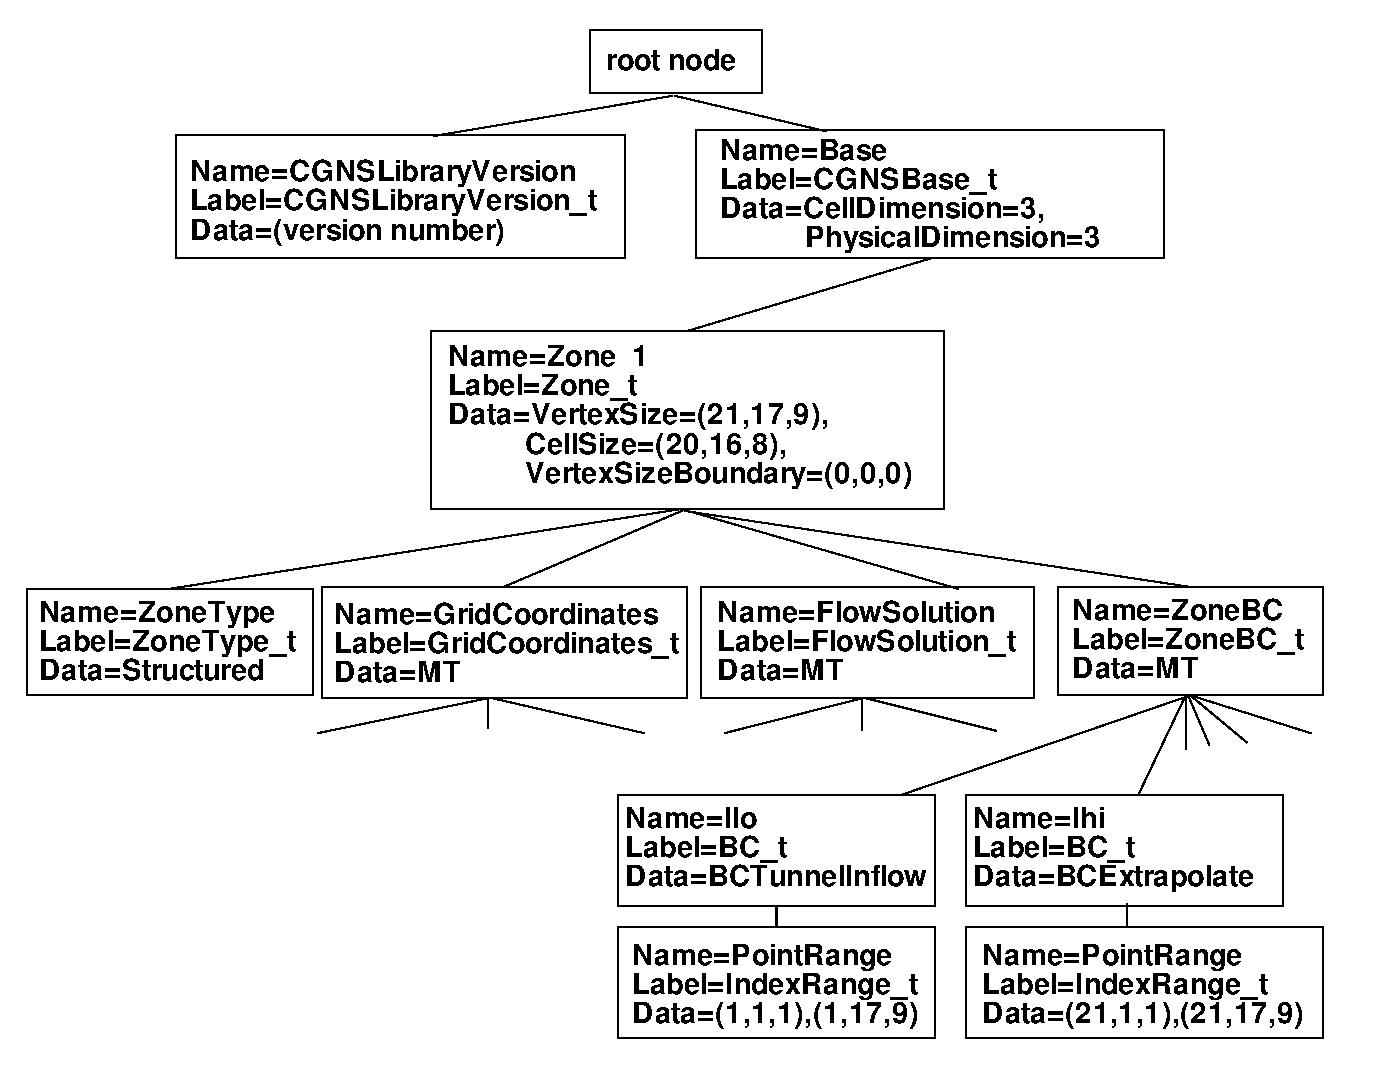
\includegraphics[width=150mm]{figures/tree_cartesian_BC}}}
\caption{Layout of CGNS file 
for simple Cartesian structured grid with flow
solution and boundary conditions using {\tt PointRange}.}
\label{FIGtree_cartesian_BC}
\end{figure}
%

Reading the boundary conditions can also be easily accomplished using
API calls, but we do not show an example of this here.
Because there are multiple {\tt BC\_t} children nodes under the
{\tt ZoneBC\_t} node, the user must first read in the number
of children nodes 
that exist, then loop through them and retrieve the information
from each.

~

\noindent\underbar{(b) Boundary Conditions Specifying Points}

The FORTRAN code segment to write the boundary conditions using
{\tt PointList} is the same as that for {\tt PointRange} except
that the following segment, for example,

--------------------------------------------------------------------

{\tt \noindent c  write boundary conditions for ilo face, defining range first
\newline c  (user can give any name)
\newline\indent      ipnts(1,1)=ilo
\newline\indent      ipnts(2,1)=jlo
\newline\indent      ipnts(3,1)=klo
\newline\indent      ipnts(1,2)=ilo
\newline\indent      ipnts(2,2)=jhi
\newline\indent      ipnts(3,2)=khi
\newline\indent      call cg\_boco\_write\_f(index\_file,index\_base,index\_zone,'Ilo',
\newline + \indent BCTunnelInflow,PointRange,2,ipnts,index\_bc,ier)}

--------------------------------------------------------------------

\noindent is replaced by:

--------------------------------------------------------------------

{\tt \noindent c  write boundary conditions for ilo face, defining pointlist first 
\newline c  (user can give any name)
\newline\indent   icount=0
\newline\indent   do j=jlo,jhi
\newline\indent\indent     do k=klo,khi
\newline\indent\indent\indent       icount=icount+1
\newline\indent\indent\indent       ipnts(1,icount)=ilo
\newline\indent\indent\indent       ipnts(2,icount)=j
\newline\indent\indent\indent       ipnts(3,icount)=k
\newline\indent\indent     enddo
\newline\indent   enddo
\newline\indent      call cg\_boco\_write\_f(index\_file,index\_base,index\_zone,'Ilo',
\newline + \indent BCTunnelInflow,PointList,icount,ipnts,index\_bc,ier)}

--------------------------------------------------------------------

\noindent The layout of the CGNS file in this case is the same as
Fig.~\ref{FIGtree_cartesian_BC}, except that {\tt PointRange}
({\tt IndexRange\_t}) becomes {\tt PointList} ({\tt IndexArray\_t})
and there is {\tt icount} data in
the {\tt PointList} nodes.

\subsubsection{Multi-Zone Structured Grid with 1-to-1 Connectivity} \label{sec:str1to1}

For the case of a multi-zone structured grid, each zone is
handled individually in the same way as the examples in the preceding
sections.  However, multi-zone grids also require additional
information about how the zones are connected to one another.
A discussion of different types of zone-to-zone connectivity can be found
in Appendix~\ref{sec:sidsoverview}.  For the example in this section, we show only
a simple 1-to-1 connectivity example.  We assume that we have a two-zone
grid, each identical to the one showed in Fig.~\ref{FIGgrid_cartesian}
($21 \times 17 \times 9$), except that zone 2 is offset in the
$x$-direction by 20 units.  Thus, the $ilo$ face of zone 2 abuts
the $ihi$ face of zone 1, and each abutting point in the two zones 
touches a point from the neighboring zone.
A picture of the grid is shown in
Fig.~\ref{FIGgrid_cartesian2}.

% Figure
\begin{figure}[hpbt]
\centerline{{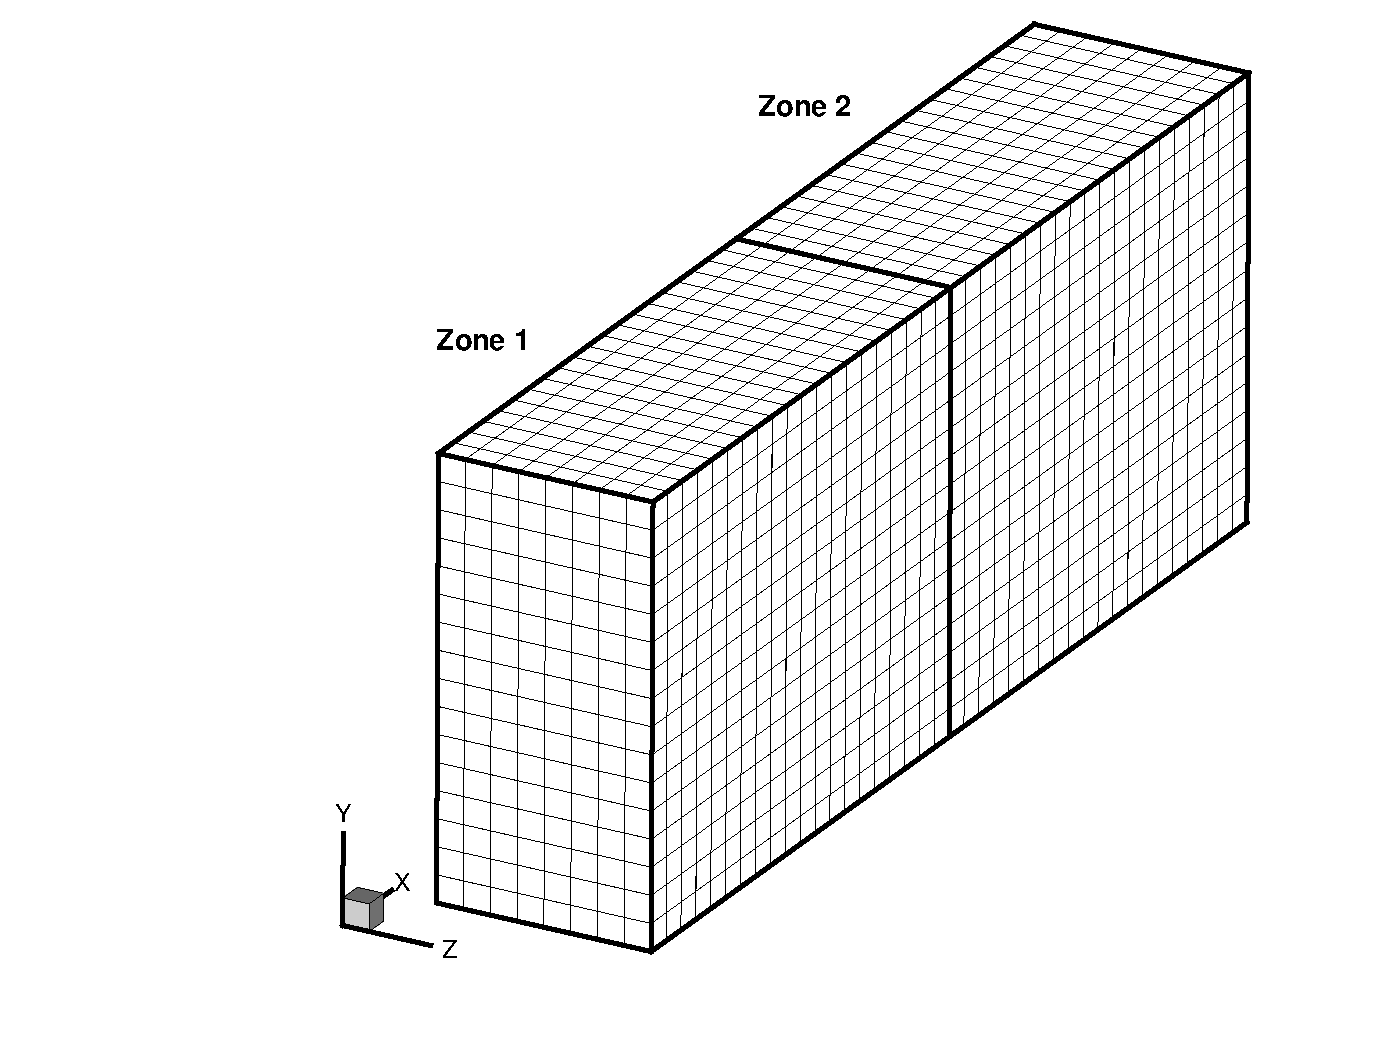
\includegraphics[width=120mm]{figures/grid_cartesian2}}}
\caption{2-Zone Cartesian structured grid with 1-to-1 connectivity.}
\label{FIGgrid_cartesian2}
\end{figure}
%

The overall layout of this two-zone CGNS file is not shown here.
It is similar to those shown earlier, except now there are two
zones rather than one.  See Appendix~\ref{sec:sidsoverview} for an additional example.

Now, 1-to-1 connectivity information must be written into
each of the zones.  There are two ways to record this 1-to-1
information.
The first (specific)
method is valid only for 1-to-1 interfaces, and the regions
{\it must} be logically rectangular (because they are recorded
via {\tt PointRange} and {\tt PointRangeDonor}
nodes, for which only two points define
the entire region). 
The second way is more general.  It uses 
{\tt PointList} nodes in combination with {\tt PointListDonor}.
(A third method, used to describe interfaces that are
{\it not} point-matched -- such as mismatched or overset zones --
employs {\tt CellListDonor} and {\tt InterpolantsDonor}.)
Refer to the SIDS document \cite{ALLMARAS}
for details on the various methods for describing connectivity.

~

\noindent\underbar{(a) Connectivity Using Specific 1-to-1 Method}

The 1-to-1 connectivity information for the current example
can be written to a CGNS file using the following
FORTRAN code segment (assuming that all grid information has
already been written):

--------------------------------------------------------------------

{\tt \noindent c  WRITE 1-TO-1 CONNECTIVITY INFORMATION TO EXISTING CGNS FILE
\newline\indent      include 'cgnslib\_f.h'
\newline c  open CGNS file for modify
\newline\indent      call cg\_open\_f('grid.cgns',MODE\_MODIFY,index\_file,ier)
\newline c  we know there is only one base (real working code would check!)
\newline\indent      index\_base=1
\newline c   get number of zones (should be 2 for our case)
\newline\indent      call cg\_nzones\_f(index\_file,index\_base,nzone,ier)
\newline c   loop over zones to get zone sizes and names
\newline\indent      do index\_zone=1,nzone
\newline\indent\indent      call cg\_zone\_read\_f(index\_file,index\_base,index\_zone,
\newline \indent + \indent zonename(index\_zone),isize,ier)
\newline\indent\indent      ilo(index\_zone)=1
\newline\indent\indent      ihi(index\_zone)=isize(1,1)
\newline\indent\indent      jlo(index\_zone)=1
\newline\indent\indent      jhi(index\_zone)=isize(2,1)
\newline\indent\indent      klo(index\_zone)=1
\newline\indent\indent      khi(index\_zone)=isize(3,1)
\newline\indent      enddo
\newline c   loop over zones again
\newline\indent      do index\_zone=1,nzone
\newline c   set up index ranges
\newline\indent\indent   if (index\_zone .eq. 1) then
\newline\indent\indent\indent      donorname=zonename(2)
\newline c   lower point of receiver range
\newline\indent\indent\indent      ipnts(1,1)=ihi(1)
\newline\indent\indent\indent      ipnts(2,1)=jlo(1)
\newline\indent\indent\indent      ipnts(3,1)=klo(1)
\newline c   upper point of receiver range
\newline\indent\indent\indent      ipnts(1,2)=ihi(1)
\newline\indent\indent\indent      ipnts(2,2)=jhi(1)
\newline\indent\indent\indent      ipnts(3,2)=khi(1)
\newline c   lower point of donor range
\newline\indent\indent\indent      ipntsdonor(1,1)=ilo(2)
\newline\indent\indent\indent      ipntsdonor(2,1)=jlo(2)
\newline\indent\indent\indent      ipntsdonor(3,1)=klo(2)
\newline c   upper point of donor range
\newline\indent\indent\indent      ipntsdonor(1,2)=ilo(2)
\newline\indent\indent\indent      ipntsdonor(2,2)=jhi(2)
\newline\indent\indent\indent      ipntsdonor(3,2)=khi(2)
\newline\indent\indent   else
\newline\indent\indent\indent      donorname=zonename(1)
\newline c   lower point of receiver range
\newline\indent\indent\indent      ipnts(1,1)=ilo(2)
\newline\indent\indent\indent      ipnts(2,1)=jlo(2)
\newline\indent\indent\indent      ipnts(3,1)=klo(2)
\newline c   upper point of receiver range
\newline\indent\indent\indent      ipnts(1,2)=ilo(2)
\newline\indent\indent\indent      ipnts(2,2)=jhi(2)
\newline\indent\indent\indent      ipnts(3,2)=khi(2)
\newline c   lower point of donor range
\newline\indent\indent\indent      ipntsdonor(1,1)=ihi(1)
\newline\indent\indent\indent      ipntsdonor(2,1)=jlo(1)
\newline\indent\indent\indent      ipntsdonor(3,1)=klo(1)
\newline c   upper point of donor range
\newline\indent\indent\indent      ipntsdonor(1,2)=ihi(1)
\newline\indent\indent\indent      ipntsdonor(2,2)=jhi(1)
\newline\indent\indent\indent      ipntsdonor(3,2)=khi(1)
\newline\indent\indent   end if
\newline c   set up Transform
\newline\indent\indent      itranfrm(1)=1
\newline\indent\indent      itranfrm(2)=2
\newline\indent\indent      itranfrm(3)=3
\newline c   write 1-to-1 info (user can give any name)
\newline\indent\indent   call cg\_1to1\_write\_f(index\_file,index\_base,index\_zone,
\newline\indent + \indent 'Interface',donorname,ipnts,ipntsdonor,itranfrm,
\newline\indent + \indent index\_conn,ier)
\newline\indent      enddo
\newline c  close CGNS file
\newline\indent      call cg\_close\_f(index\_file,ier)}

--------------------------------------------------------------------

\noindent Note that this code segment is geared very specifically 
toward our 2-zone example, i.e., it relies on our
knowledge of this particular case.  {\tt Transform} defines the
relative orientation of the $i$, $j$, and $k$ indices of the
abutting zones.  Details concerning the
values of {\tt Transform} are not given here; they can be found in
\cite{ALLMARAS}.  However, note that {\tt Transform} values of 
(1,2,3) indicate that the $i$, $j$, $k$ axes of both zones
are oriented in the same directions.  Reading the connectivity information 
can also be easily accomplished using
API calls, but we do not show an example of this here.
And finally, we do not show the layout of the nodes associated with
the connectivity here.  The interested user is referred to 
Appendix~\ref{sec:sidsoverview} for an example figure.

~

\noindent\underbar{(b) Connectivity Using General Method}

Using a more general method, for which each connectivity pair is
listed (rather than ranges),
the connectivity information for the current example
can be written to a CGNS file using the following
FORTRAN code segment:

--------------------------------------------------------------------

{\tt \noindent c  WRITE GENERAL CONNECTIVITY INFORMATION TO EXISTING CGNS FILE
\newline\indent      include 'cgnslib\_f.h'
\newline c  open CGNS file for modify
\newline\indent      call cg\_open\_f('grid.cgns',MODE\_MODIFY,index\_file,ier)
\newline c  we know there is only one base (real working code would check!)
\newline\indent      index\_base=1
\newline c   get number of zones (should be 2 for our case)
\newline\indent      call cg\_nzones\_f(index\_file,index\_base,nzone,ier)
\newline c   loop over zones to get zone sizes and names
\newline\indent      do index\_zone=1,nzone
\newline\indent\indent      call cg\_zone\_read\_f(index\_file,index\_base,index\_zone,
\newline \indent + \indent zonename(index\_zone),isize,ier)
\newline\indent\indent      ilo(index\_zone)=1
\newline\indent\indent      ihi(index\_zone)=isize(1,1)
\newline\indent\indent      jlo(index\_zone)=1
\newline\indent\indent      jhi(index\_zone)=isize(2,1)
\newline\indent\indent      klo(index\_zone)=1
\newline\indent\indent      khi(index\_zone)=isize(3,1)
\newline\indent      enddo
\newline c   loop over zones again
\newline\indent      do index\_zone=1,nzone
\newline c   set up point lists
\newline\indent\indent   if (index\_zone .eq. 1) then
\newline\indent\indent\indent   icount=0
\newline\indent\indent\indent   do j=jlo(index\_zone),jhi(index\_zone)
\newline\indent\indent\indent\indent     do k=klo(index\_zone),khi(index\_zone)
\newline\indent\indent\indent\indent\indent       icount=icount+1
\newline\indent\indent\indent\indent\indent       ipnts(1,icount)=ihi(1)
\newline\indent\indent\indent\indent\indent       ipnts(2,icount)=j
\newline\indent\indent\indent\indent\indent       ipnts(3,icount)=k
\newline\indent\indent\indent\indent\indent       ipntsdonor(1,icount)=ilo(2)
\newline\indent\indent\indent\indent\indent       ipntsdonor(2,icount)=j
\newline\indent\indent\indent\indent\indent       ipntsdonor(3,icount)=k
\newline\indent\indent\indent\indent     enddo
\newline\indent\indent\indent   enddo
\newline\indent\indent\indent      donorname=zonename(2)
\newline\indent\indent   else
\newline\indent\indent\indent   icount=0
\newline\indent\indent\indent   do j=jlo(index\_zone),jhi(index\_zone)
\newline\indent\indent\indent\indent     do k=klo(index\_zone),khi(index\_zone)
\newline\indent\indent\indent\indent\indent       icount=icount+1
\newline\indent\indent\indent\indent\indent       ipnts(1,icount)=ilo(2)
\newline\indent\indent\indent\indent\indent       ipnts(2,icount)=j
\newline\indent\indent\indent\indent\indent       ipnts(3,icount)=k
\newline\indent\indent\indent\indent\indent       ipntsdonor(1,icount)=ihi(1)
\newline\indent\indent\indent\indent\indent       ipntsdonor(2,icount)=j
\newline\indent\indent\indent\indent\indent       ipntsdonor(3,icount)=k
\newline\indent\indent\indent\indent     enddo
\newline\indent\indent\indent   enddo
\newline\indent\indent\indent      donorname=zonename(1)
\newline\indent\indent   end if
\newline c   write integer connectivity info (user can give any name)
\newline\indent\indent   call cg\_conn\_write\_f(index\_file,index\_base,index\_zone,
\newline\indent + \indent 'GenInterface',Vertex,Abutting1to1,PointList,icount,ipnts,
\newline\indent + \indent donorname,Structured,PointListDonor,Integer,icount,
\newline\indent + \indent ipntsdonor,index\_conn,ier)
\newline\indent      enddo
\newline c  close CGNS file
\newline\indent      call cg\_close\_f(index\_file,ier)}

--------------------------------------------------------------------

\noindent
We do not describe the method for recording mismatched (patched) or
overset connectivity information in this document;
the user is referred to \cite{ALLMARAS} for details.  However, note that
in such cases the use of {\tt CellListDonor} (along with {\tt InterpolantsDonor})
implies the specification of {\it cell center indices} on the donor
side (these would correspond to element numbers in
unstructured zones).  The {\tt InterpolantsDonor} information consists of
real-valued interpolants.

\newpage
\subsection{Unstructured Grid} \label{sec:unstr}

This section gives several unstructured grid examples.
The user should already be familiar with the information
covered in section~\ref{sec:str}, which gives structured grid examples.
Because much of the organization of the
CGNS files is identical for both grid types, many
of the ideas covered in the structured grid section
are not repeated again here.

\subsubsection{Single-Zone Unstructured Grid} \label{sec:unstrgrid}

This example uses the exact same grid shown
earlier in Fig.~\ref{FIGgrid_cartesian}.  However, it is now written
as an {\it unstructured} grid, which is made up of a series
of 6-sided elements (cubes in this case).
A FORTRAN code segment that uses API calls to write this grid
to a CGNS file called {\tt grid.cgns} is shown here (note that it {\it does not matter}
how the nodes are ordered in an unstructured zone, but in this 
example they are ordered sequentially for simplicity of presentation):

--------------------------------------------------------------------

{\tt \noindent c  WRITE X, Y, Z GRID POINTS TO CGNS FILE
\newline\indent      include 'cgnslib\_f.h'
\newline c  open CGNS file for write
\newline\indent      call cg\_open\_f('grid.cgns',MODE\_WRITE,index\_file,ier)
\newline c  create base (user can give any name)
\newline\indent      basename='Base'
\newline\indent      icelldim=3
\newline\indent      iphysdim=3
\newline\indent      call cg\_base\_write\_f(index\_file,basename,icelldim,iphysdim,index\_base,ier)
\newline c  define zone name (user can give any name)
\newline\indent      zonename = 'Zone~~1'
\newline c  We use the same grid as for the structured example with ni=21,
\newline c  nj=17, nk=9.  The variables ni, nj, and nk are still used later,
\newline c  for convenience when numbering the unstructured grid elements.
\newline\indent      ni=21
\newline\indent      nj=17
\newline\indent      nk=9
\newline c  vertex size (21*17*9 = 3213)
\newline\indent      isize(1,1)=3213
\newline c  cell size (20*16*8 = 2560)
\newline\indent      isize(1,2)=2560
\newline c  boundary vertex size (zero if elements not sorted)
\newline\indent      isize(1,3)=0
\newline c  create zone
\newline\indent      call cg\_zone\_write\_f(index\_file,index\_base,zonename,isize,
\newline + \indent Unstructured,index\_zone,ier)
\newline c  write grid coordinates (user must use SIDS-standard names here)
\newline\indent      call cg\_coord\_write\_f(index\_file,index\_base,index\_zone,RealDouble,
\newline + \indent 'CoordinateX',x,index\_coord,ier)
\newline\indent      call cg\_coord\_write\_f(index\_file,index\_base,index\_zone,RealDouble,
\newline + \indent 'CoordinateY',y,index\_coord,ier)
\newline\indent      call cg\_coord\_write\_f(index\_file,index\_base,index\_zone,RealDouble,
\newline + \indent 'CoordinateZ',z,index\_coord,ier)
\newline c  set element connectivity:
\newline c  do all the HEXA\_8 elements (this part is mandatory):
\newline c  maintain SIDS-standard ordering
\newline\indent   ielem\_no=0
\newline c  index no of first element
\newline\indent      nelem\_start=1
\newline\indent   do k=1,nk-1
\newline\indent\indent   do j=1,nj-1
\newline\indent\indent\indent   do i=1,ni-1
\newline\indent\indent\indent\indent     ielem\_no=ielem\_no+1
\newline c  in this example, due to the order in the node numbering, the
\newline c  hexahedral elements can be reconstructed using the following
\newline c  relationships:
\newline\indent\indent\indent\indent     ifirstnode=i+(j-1)*ni+(k-1)*ni*nj
\newline\indent\indent\indent\indent     ielem(1,ielem\_no)=ifirstnode
\newline\indent\indent\indent\indent     ielem(2,ielem\_no)=ifirstnode+1
\newline\indent\indent\indent\indent     ielem(3,ielem\_no)=ifirstnode+1+ni
\newline\indent\indent\indent\indent     ielem(4,ielem\_no)=ifirstnode+ni
\newline\indent\indent\indent\indent     ielem(5,ielem\_no)=ifirstnode+ni*nj
\newline\indent\indent\indent\indent     ielem(6,ielem\_no)=ifirstnode+ni*nj+1
\newline\indent\indent\indent\indent     ielem(7,ielem\_no)=ifirstnode+ni*nj+1+ni
\newline\indent\indent\indent\indent     ielem(8,ielem\_no)=ifirstnode+ni*nj+ni
\newline\indent\indent\indent   enddo
\newline\indent\indent   enddo
\newline\indent   enddo
\newline c  index no of last element (=2560)
\newline\indent      nelem\_end=ielem\_no
\newline c  unsorted boundary elements
\newline\indent      nbdyelem=0
\newline c  write HEXA\_8 element connectivity (user can give any name)
\newline\indent      call cg\_section\_write\_f(index\_file,index\_base,index\_zone,
\newline + \indent 'Elem',HEXA\_8,nelem\_start,nelem\_end,nbdyelem,ielem,
\newline + \indent index\_section,ier)
\newline c  close CGNS file
\newline\indent      call cg\_close\_f(index\_file,ier)}

--------------------------------------------------------------------

Note that for unstructured zones, the index dimension is always 1
(because only one index value is required to identify a position
in the mesh),
so the {\tt isize} array contains the total vertex size, cell size,
and boundary vertex size for the zone.
In this example, the {\tt ielem} array must be dimensioned exactly
as (8,$N$), where $N$ is greater than or equal to the total number
of elements.
The node points that lie in the lower left corner of 
Fig.~\ref{FIGgrid_cartesian} are shown schematically
for two elements in Fig.~\ref{FIGgrid_cartesianU}.
Here it can be seen, for example, that node numbers
1, 2, 23, 22, 358, 359, 380, and 379 make up element 1.

% Figure
\begin{figure}[hpbt]
\centerline{{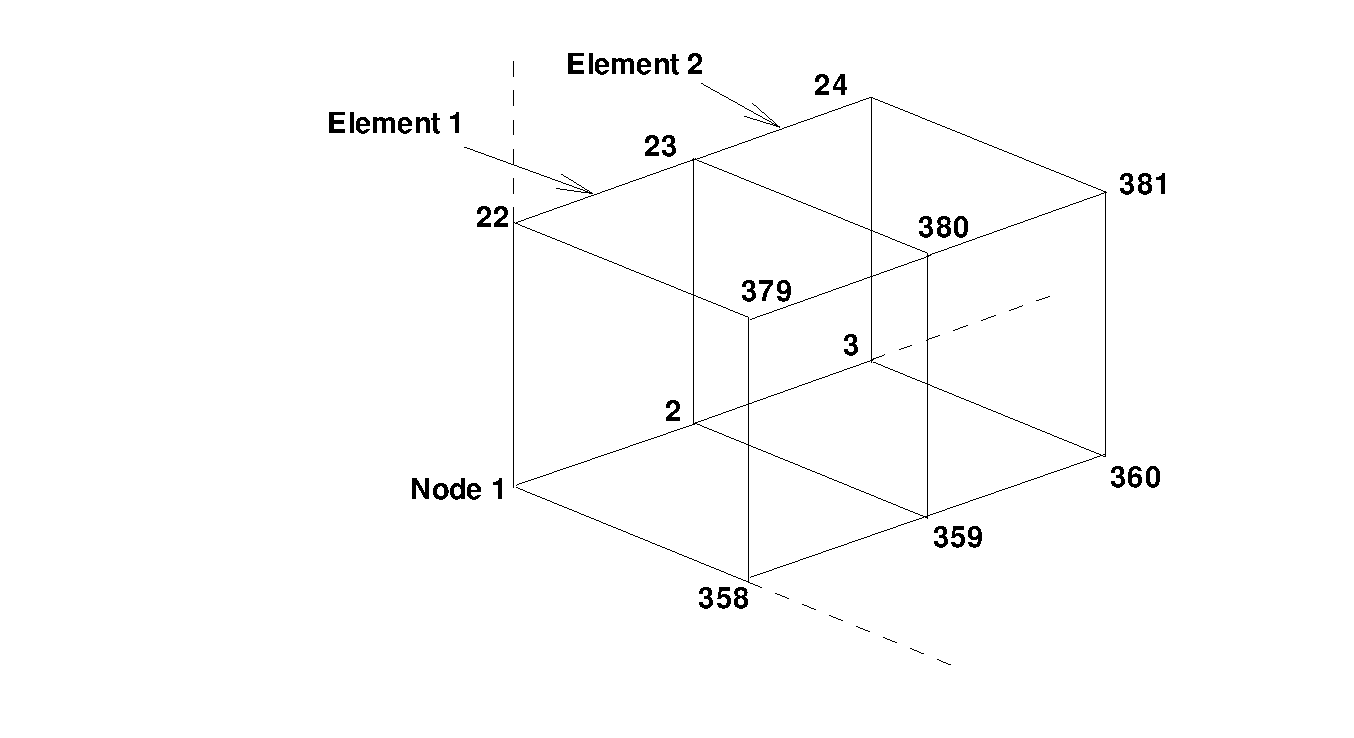
\includegraphics[width=150mm]{figures/grid_cartesianU}}}
\caption{Schematic representation of nodes and elements of unstructured grid.}
\label{FIGgrid_cartesianU}
\end{figure}
%

The overall layout of the CGNS file created by the above code segment
is shown in Fig.~\ref{FIGtree_cartesianU}.  The nodes for {\tt y} and
{\tt z} are left off due to lack of space.  
Compare this figure with the
layout for the structured version of this grid in
Fig.~\ref{FIGtree_cartesian}.

% Figure
\begin{figure}[hpbt]
\centerline{{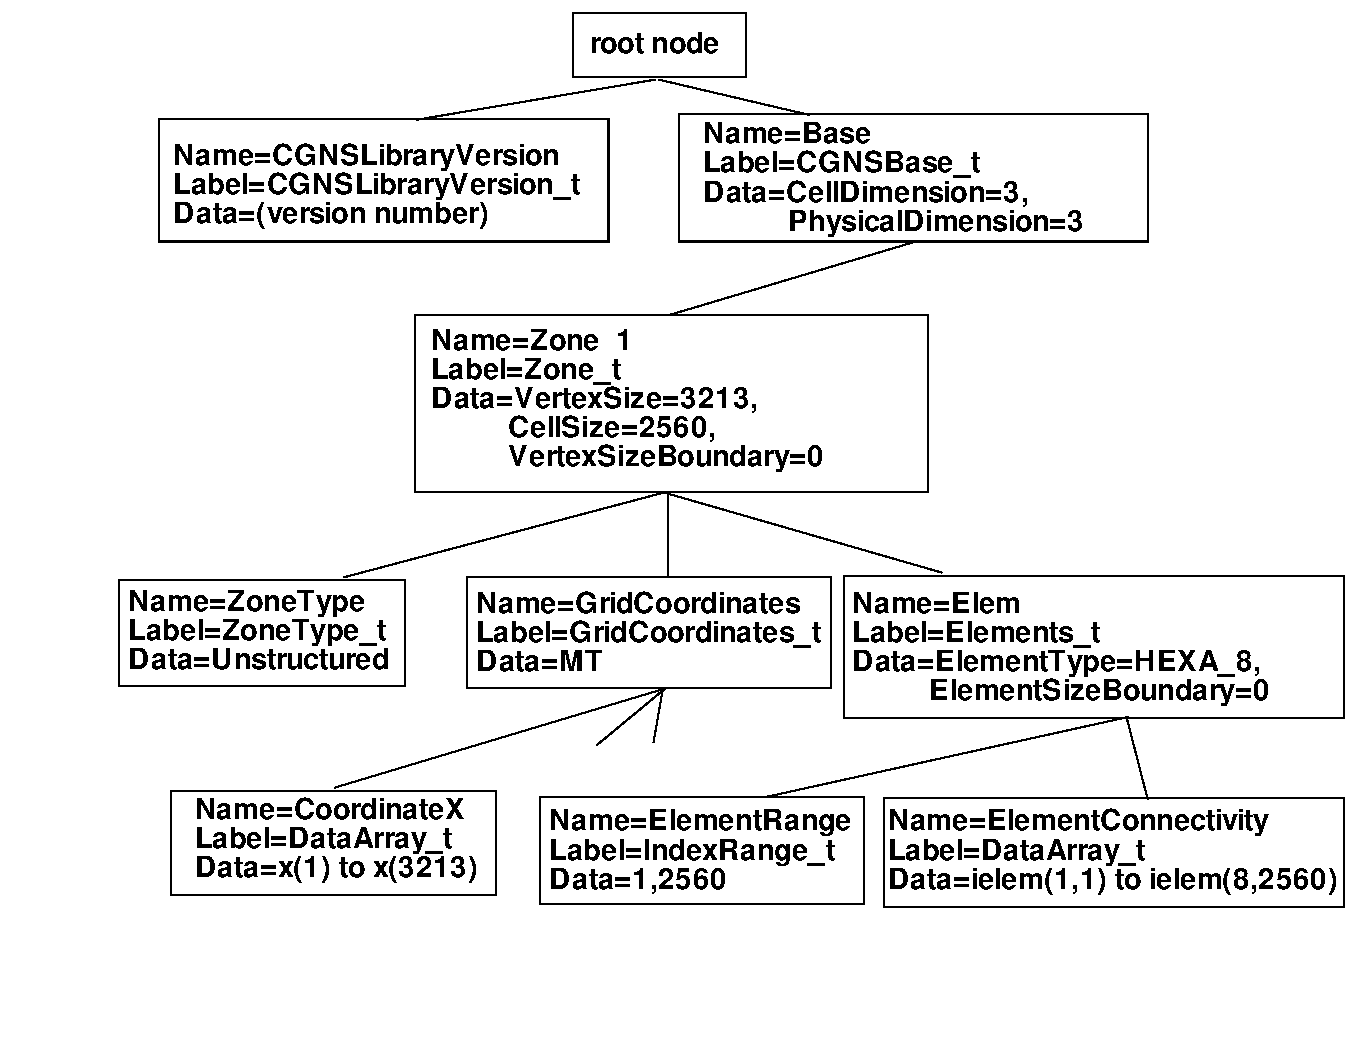
\includegraphics[width=150mm]{figures/tree_cartesianU}}}
\caption{Layout of CGNS file for unstructured grid.}
\label{FIGtree_cartesianU}
\end{figure}
%

For unstructured zones, the user may also wish to separately list the
boundary elements in the CGNS file.  This may be useful for assigning boundary
conditions, as we will show in section~\ref{sec:bcunstr} below.
In the current example, assume that the user wishes to assign three
different types of boundary conditions: inflow at one end,
outflow at the other end, and side walls on the four
faces in-between.  To accomplish this, it would be helpful to have three
additional {\tt Elements\_t} nodes in the CGNS file, each of which lists the 
corresponding faces as elements ({\tt QUAD\_4} in this case). 

A FORTRAN code segment that accomplishes a part of this is given here.  It may
be a part of the same code (above) that defined the grid and {\tt HEXA\_8}
connectivity.

--------------------------------------------------------------------

{\tt \noindent c  do boundary (QUAD) elements (this part is optional,
\newline c  but you must do it if you eventually want to define BCs
\newline c  at element faces rather than at nodes):
\newline c  INFLOW:
\newline\indent      ielem\_no=0
\newline c  index no of first element
\newline\indent      nelem\_start=nelem\_end+1
\newline\indent      i=1
\newline\indent      do k=1,nk-1
\newline\indent\indent        do j=1,nj-1
\newline\indent\indent\indent          ielem\_no=ielem\_no+1
\newline\indent\indent\indent          ifirstnode=i+(j-1)*ni+(k-1)*ni*nj
\newline\indent\indent\indent          jelem(1,ielem\_no)=ifirstnode
\newline\indent\indent\indent          jelem(2,ielem\_no)=ifirstnode+ni*nj
\newline\indent\indent\indent          jelem(3,ielem\_no)=ifirstnode+ni*nj+ni
\newline\indent\indent\indent          jelem(4,ielem\_no)=ifirstnode+ni
\newline\indent\indent        enddo
\newline\indent      enddo
\newline c  index no of last element
\newline\indent      nelem\_end=nelem\_start+ielem\_no-1
\newline c  write QUAD element connectivity for inflow face (user can give any name)
\newline\indent      call cg\_section\_write\_f(index\_file,index\_base,index\_zone,
\newline + \indent   'InflowElem',QUAD\_4,nelem\_start,nelem\_end,nbdyelem,
\newline + \indent   jelem,index\_section,ier)
\newline c  OUTFLOW:
\newline\indent\indent  ... etc...
}

--------------------------------------------------------------------

In this example, the {\tt jelem} array must be dimensioned exactly
as (4,$N$), where $N$ is greater than or equal to the total number
of elements.  Note that the {\tt nelem\_start} and {\tt nelem\_end}
range is defined {\it subsequent} to the range of any other
elements (i.e., the {\tt HEXA\_8} elements) already defined in this zone.
In other words, all elements in a given zone must have a different
number.

The layout of the CGNS file in this case is exactly the same as that shown
in Fig.~\ref{FIGtree_cartesianU}, except that there are now three additional
{\tt Elements\_t} nodes under {\tt Zone\_t}.  These are shown separately in 
Fig.~\ref{FIGtree_cartesianUelem}.

% Figure
\begin{figure}[hpbt]
\centerline{{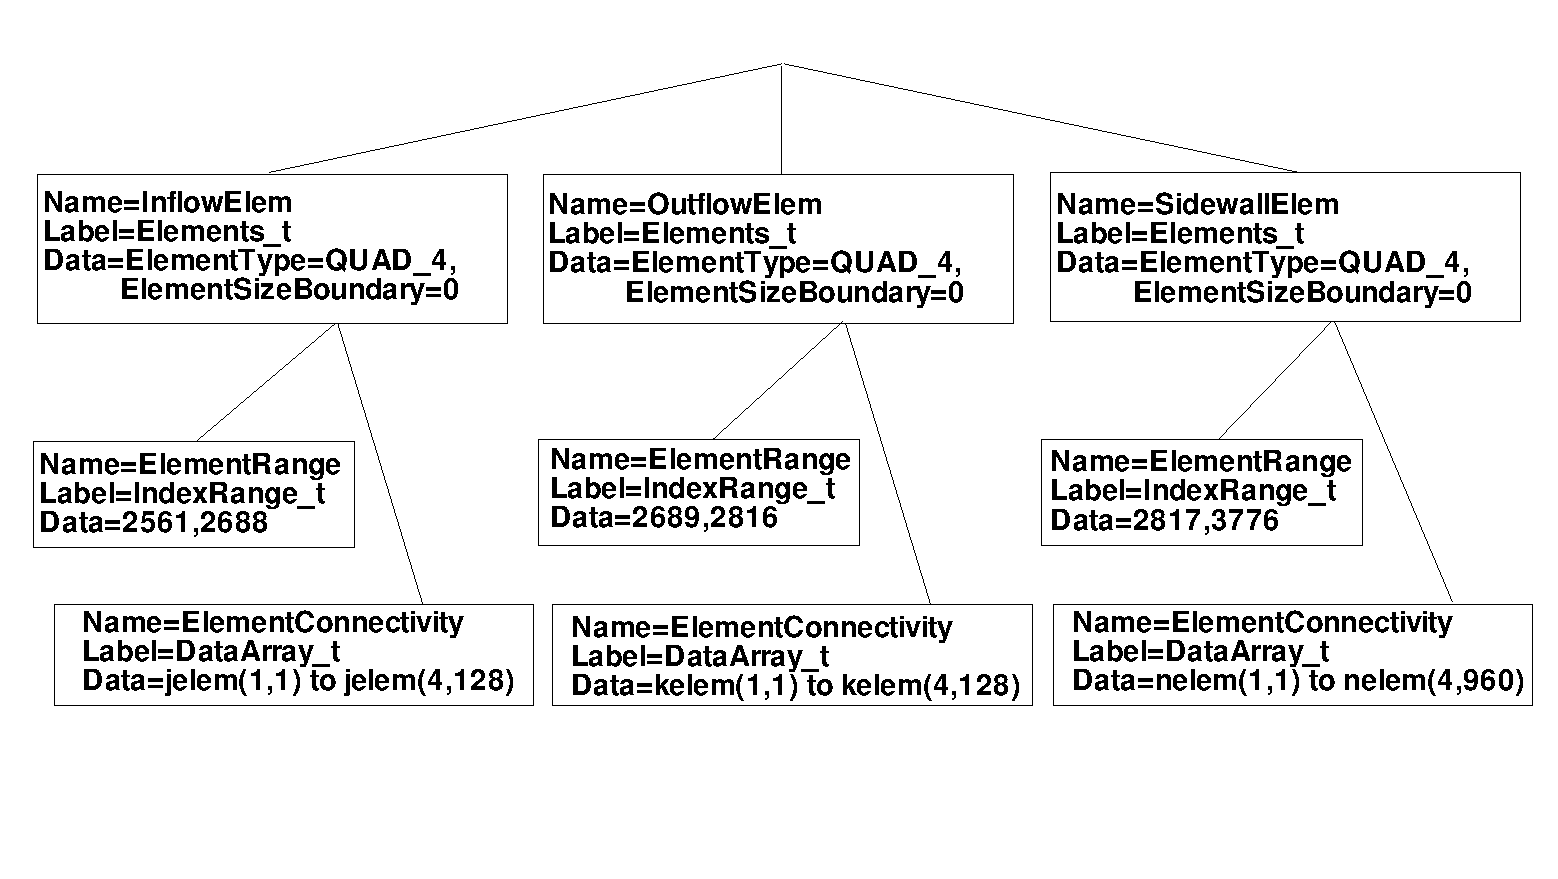
\includegraphics[width=150mm]{figures/tree_cartesianUelem}}}
\caption{Layout of additional {\tt Elements\_t} boundary face nodes.}
\label{FIGtree_cartesianUelem}
\end{figure}
%

\subsubsection{Single-Zone Unstructured Grid and Flow Solution} \label{sec:unstrflow}

To add a flow solution to an unstructured zone, the procedure is
identical to that for a structured zone.  However, the Rind field for unstructured
grids indicates additional points rather than planes. Example of Rind capability for unstructured
grids is not covered here.
Considering the vertex and cell-center examples shown in section~\ref{sec:flowsoln}, the
only difference for unstructured zones is that
all arrays are one-dimensional (there is only one index), as opposed to three 
indices for 3-D structured arrays.  A vertex solution indicates that the solution
is stored at vertices or nodes.  In the above example, 
there would be lists of 3213
data array items per solution variable.  A cell center solution implies that the solution
is stored at the center of each element.  In the above example, 
there would be lists of 2560 data array items per solution variable.

The overall layout of the CGNS file is the same as that shown in 
Fig.~\ref{FIGtree_cartesianU}, except that there would also be a
{\tt FlowSolution\_t} node under {\tt Zone~~1}, and this node would
have the children nodes {\tt GridLocation},
{\tt Density}, and {\tt Pressure}.

\subsubsection{Single-Zone Unstructured Grid with Boundary Conditions} \label{sec:bcunstr}

When writing boundary conditions to a CGNS file for an unstructured
zone, one can follow the same general procedure outlined in
section~\ref{sec:bcstruct} for a structured zone.
In other words, the boundary conditions can be defined for point ranges or
for individual points, where the points refer to nodes (vertices) of the
grid.
Coding would be essentially the same as that presented in
section~\ref{sec:bcstruct}, except that the points and/or ranges are now
one-dimensional (there is only one index), as opposed to three indices
for 3-D structured arrays.

However, for unstructured zones this is generally not the recommended method.
Usually, for unstructured zones one has also already defined
additional {\tt Elements\_t} nodes that {\it define} the boundary face elements
(see section~\ref{sec:unstrgrid}).
Therefore, it is best for the boundary conditions to be associated with
these elements rather than with the nodes.

Because this concept is quite different from what was done with the
structured zone earlier, we illustrate it with an example.  At the end
of section~\ref{sec:unstrgrid}, we showed how to create the additional
{\tt Elements\_t} nodes defining the boundary faces.  The face-center
boundary conditions now can be written using the following code segment.

--------------------------------------------------------------------

{\tt \noindent c  WRITE BOUNDARY CONDITIONS TO EXISTING CGNS FILE
\newline\indent      include 'cgnslib\_f.h'
\newline c  open CGNS file for modify
\newline\indent      call cg\_open\_f('grid.cgns',MODE\_MODIFY,index\_file,ier)
\newline c  we know there is only one base (real working code would check!)
\newline\indent      index\_base=1
\newline c  we know there is only one zone (real working code would check!)
\newline\indent      index\_zone=1
\newline c  we know that for the unstructured zone, the following face elements
\newline c  have been defined as inflow (real working code would check!):
\newline\indent      nelem\_start=2561
\newline\indent      nelem\_end=2688
\newline\indent      icount=0
\newline\indent      do n=nelem\_start,nelem\_end
\newline\indent\indent        icount=icount+1
\newline\indent\indent        ipnts(icount)=n
\newline\indent      enddo
\newline c  write boundary conditions for ilo face
\newline\indent      call cg\_boco\_write\_f(index\_file,index\_base,index\_zone,'Ilo',
\newline + \indent BCTunnelInflow,ElementList,icount,ipnts,index\_bc,ier)
\newline c  we know that for the unstructured zone, the following face elements
\newline c  have been defined as outflow (real working code would check!):
\newline\indent      nelem\_start=2689
\newline\indent      nelem\_end=2816
\newline\indent      icount=0
\newline\indent      do n=nelem\_start,nelem\_end
\newline\indent\indent        icount=icount+1
\newline\indent\indent        ipnts(icount)=n
\newline\indent      enddo
\newline c  write boundary conditions for ihi face
\newline\indent      call cg\_boco\_write\_f(index\_file,index\_base,index\_zone,'Ihi',
\newline + \indent BCExtrapolate,ElementList,icount,ipnts,index\_bc,ier)
\newline c  we know that for the unstructured zone, the following face elements
\newline c  have been defined as walls (real working code would check!):
\newline\indent      nelem\_start=2817
\newline\indent      nelem\_end=3776
\newline\indent      icount=0
\newline\indent      do n=nelem\_start,nelem\_end
\newline\indent\indent        icount=icount+1
\newline\indent\indent        ipnts(icount)=n
\newline\indent      enddo
\newline c  write boundary conditions for wall faces
\newline\indent      call cg\_boco\_write\_f(index\_file,index\_base,index\_zone,'Walls',
\newline + \indent BCWallInviscid,ElementList,icount,ipnts,index\_bc,ier)
\newline c
\newline c  close CGNS file
\newline\indent      call cg\_close\_f(index\_file,ier)
}

--------------------------------------------------------------------

Note that we assume here that we know in advance the element numbers
associated with each of the boundaries.
We have written these element numbers as a {\tt ElementList}, but, because
they are in order, we could just as easily have used {\tt ElementRange}
instead.
In that case, only two {\tt ipnts} values would be needed, equal to
{\tt nelem\_start} and {\tt nelem\_end}, and {\tt icount} would be 2.

Note that it is also allowable to use {\tt PointList} or {\tt PointRange}
{\it in addition to} setting {\tt GridLocation} to {\tt FaceCenter}.
This combination has the meaning of pointing to elements rather than
to vertices because, by default,
boundary conditions are assumed to apply at vertices (nodes);
but when {\tt GridLocation} is something other than {\tt Vertex},
then the boundary conditions for an unstructured
zone no longer refer to nodes, but to elements.

A portion of the layout of the CGNS file for the {\tt ZoneBC\_t}
node and its children is shown in Fig.~\ref{FIGtree_cartesian_UBC}.  The {\tt ZoneBC\_t}
node lies directly under {\tt Zone\_t}.  The three figures,
Figs.~\ref{FIGtree_cartesianU}, \ref{FIGtree_cartesianUelem}, and
\ref{FIGtree_cartesian_UBC} taken together, constitute the entire layout of
the file.

% Figure
\begin{figure}[hpbt]
\centerline{{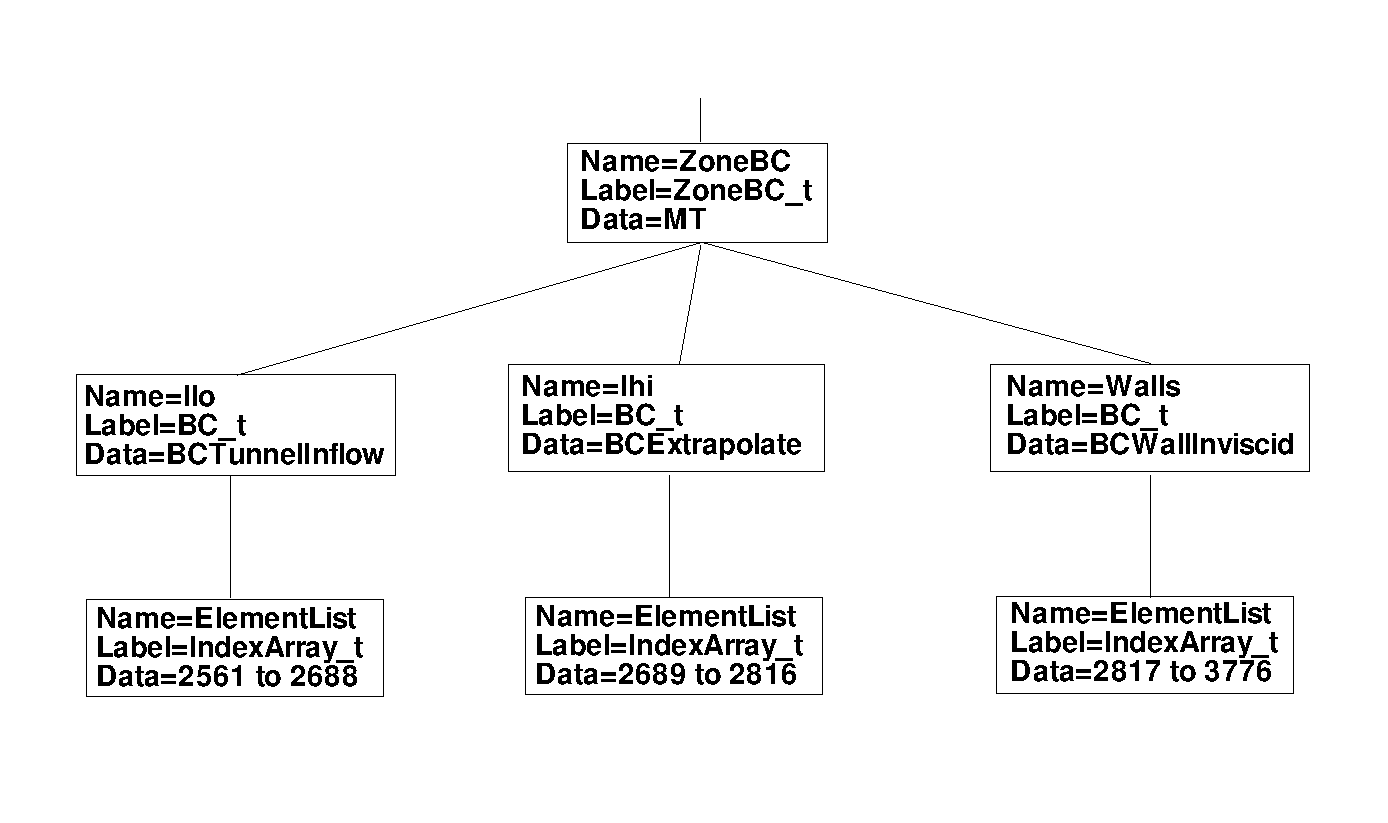
\includegraphics[width=150mm]{figures/tree_cartesian_UBC}}}
\caption{Layout of part of CGNS file for an unstructured zone with
boundary conditions defined at face-center elements.}
\label{FIGtree_cartesian_UBC}
\end{figure}
%

\newpage
\section{ADDITIONAL INFORMATION} \label{sec:advanced}

This section introduces several additional types of data in CGNS.
These items are by no means necessary to include when getting
started, but it is likely that most users will eventually want
to implement some of them into their CGNS files at some point in the future.
The section ends with a discussion on the usage of links.

\subsection{Convergence History} \label{sec:converge}

The {\tt ConvergenceHistory\_t} node can be used to store
data associated with the convergence of a CFD solution. 
For example, one may wish to store the global coefficient of lift
as a function of iterations.  In this case, 
this variable should be stored at the {\tt CGNSBase\_t} level
of the CGNS file.
This is achieved using the API in the following FORTRAN code 
segment:

--------------------------------------------------------------------

{\tt \noindent c  WRITE CONVERGENCE HISTORY INFORMATION TO EXISTING CGNS FILE
\newline\indent      include 'cgnslib\_f.h'
\newline c  open CGNS file for modify
\newline\indent      call cg\_open\_f('grid.cgns',MODE\_MODIFY,index\_file,ier)
\newline c  we know there is only one base (real working code would check!)
\newline\indent      index\_base=1
\newline c   go to base node
\newline\indent      call cg\_goto\_f(index\_file,index\_base,ier,'end')
\newline c   create history node (SIDS names it GlobalConvergenceHistory at base level)
\newline c   ntt is the number of recorded iterations
\newline\indent      call cg\_convergence\_write\_f(ntt,'',ier)
\newline c   go to new history node
\newline\indent      call cg\_goto\_f(index\_file,index\_base,ier,'ConvergenceHistory\_t',
\newline + \indent 1,'end')
\newline c   write lift coefficient array (user must use SIDS-standard name here)
\newline\indent      call cg\_array\_write\_f('CoefLift',RealDouble,1,ntt,cl,ier)
\newline c  close CGNS file
\newline\indent      call cg\_close\_f(index\_file,ier)}

--------------------------------------------------------------------

\noindent In this example, the array {\tt cl} must be declared as 
an array of size {\tt ntt} or larger.  Additional arrays {\it of the same
size} may also be written under the {\tt ConvergenceHistory\_t}
node.  Note that the call to {\tt cg\_convergence\_write\_f}
includes a blank string in this case, because we are not recording
norm definitions.

\subsection{Descriptor Nodes} \label{sec:descript}

Descriptor nodes, which record character strings and can be
inserted nearly everywhere in a CGNS file, have many 
possible uses.
Users can insert comments or descriptions
to help clarify the content of some data in the CGNS file.  In Appendix~\ref{sec:sidsoverview},
we mention a possible use for descriptor nodes to describe
data that is {\tt UserDefinedData\_t}.
Another potentially desirable use of the descriptor node is
to maintain copies of the entire {\it input} file(s)
from the CFD application code.  Because descriptor nodes
can include carriage returns, entire ASCII files can be 
``swallowed'' into the CGNS file.  In this way, a future user
can see and retrieve the exact input file(s) used by
the CFD code to generate
the data contained in the CGNS file.  The only ambiguity
possible would be whether the CFD code itself has changed since
that time; but if the CFD code has strict version control,
then complete recoverability should be possible.

An example that writes a descriptor node at the {\tt CGNSBase\_t} level
is given here:

--------------------------------------------------------------------

{\tt \noindent c  WRITE DESCRIPTOR NODE AT BASE LEVEL
\newline\indent      include 'cgnslib\_f.h'
\newline c  open CGNS file for modify
\newline\indent      call cg\_open\_f('grid.cgns',MODE\_MODIFY,index\_file,ier)
\newline c  we know there is only one base (real working code would check!)
\newline\indent      index\_base=1
\newline c   go to base node
\newline\indent      call cg\_goto\_f(index\_file,index\_base,ier,'end')
\newline c   write descriptor node (user can give any name)
\newline\indent      text1='Supersonic vehicle with landing gear'
\newline\indent      text2='M=4.6, Re=6 million'
\newline\indent      textstring=text1//char(10)//text2
\newline\indent      call cg\_descriptor\_write\_f('Information',textstring,ier)
\newline c  close CGNS file
\newline\indent      call cg\_close\_f(index\_file,ier)}

--------------------------------------------------------------------

\noindent In this example, the {\tt Descriptor\_t} node
is named {\tt Information} and
the character string {\tt textstring} (which is made up of {\tt text1}
and {\tt text2} with a line feed -- {\tt char(10)} -- in-between) is written there.
All character strings must be declared appropriately.

\subsection{Dimensional Data} \label{sec:dimens}

The node {\tt DataClass\_t} denotes the class of the data.  When
data is dimensional, then {\tt DataClass\_t} = {\tt Dimensional}.
The {\tt DataClass\_t} node can appear at many levels in the CGNS
hierarchy; precedence rules dictate that a {\tt DataClass\_t}
lower in the hierarchy supersedes any higher up.

For dimensional data, one generally is expected to indicate the
dimensionality of each particular variable through the use of
{\tt DataClass\_t}, {\tt DimensionalUnits\_t}, and
{\tt DimensionalExponents\_t}.  An example of this is
shown in the following code segment in which units are added
to the structured grid and cell center flow solution from 
sections~\ref{sec:singlegrid} and \ref{sec:flowsoln}.

--------------------------------------------------------------------

{\tt
\noindent c   WRITE DIMENSIONAL INFO FOR GRID AND FLOW SOLN
\newline\indent      include 'cgnslib\_f.h'
\newline c   open CGNS file for modify
\newline\indent      call cg\_open\_f('grid.cgns',MODE\_MODIFY,index\_file,ier)
\newline c   we know there is only one base (real working code would check!)
\newline\indent      index\_base=1
\newline c   we know there is only one zone (real working code would check!)
\newline\indent      index\_zone=1
\newline c   we know there is only one FlowSolution\_t (real working code would check!)
\newline\indent      index\_flow=1
\newline c   we know there is only one GridCoordinates\_t (real working code would check!)
\newline\indent      index\_grid=1
\newline c   put DataClass and DimensionalUnits under Base
\newline\indent      call cg\_goto\_f(index\_file,index\_base,ier,'end')
\newline\indent      call cg\_dataclass\_write\_f(Dimensional,ier)
\newline\indent      call cg\_units\_write\_f(Kilogram,Meter,Second,Kelvin,Degree,ier)
\newline c   read fields
\newline\indent      call cg\_nfields\_f(index\_file,index\_base,index\_zone,index\_flow,
\newline + \indent  nfields,ier)
\newline\indent      do if=1,nfields
\newline\indent\indent        call cg\_field\_info\_f(index\_file,index\_base,index\_zone,
\newline + \indent\indent   index\_flow,if,idatatype,fieldname,ier)
\newline\indent\indent        if (fieldname .eq. 'Density') then
\newline\indent\indent\indent          exponents(1)=1.
\newline\indent\indent\indent          exponents(2)=-3.
\newline\indent\indent\indent          exponents(3)=0.
\newline\indent\indent\indent          exponents(4)=0.
\newline\indent\indent\indent          exponents(5)=0.
\newline\indent\indent        else if (fieldname .eq. 'Pressure') then
\newline\indent\indent\indent          exponents(1)=1.
\newline\indent\indent\indent          exponents(2)=-1.
\newline\indent\indent\indent          exponents(3)=-2.
\newline\indent\indent\indent          exponents(4)=0.
\newline\indent\indent\indent          exponents(5)=0.
\newline\indent\indent        else
\newline\indent\indent\indent          write(6,'('' Error! this fieldname not expected: '',a32)')
\newline + \indent\indent\indent     fieldname
\newline\indent\indent\indent          stop
\newline\indent\indent        end if
\newline c   write DimensionalExponents
\newline\indent\indent        call cg\_goto\_f(index\_file,index\_base,ier,'Zone\_t',1,
\newline + \indent\indent   'FlowSolution\_t',1,'DataArray\_t',if,'end')
\newline\indent\indent        call cg\_exponents\_write\_f(RealSingle,exponents,ier)
\newline\indent      enddo
\newline c   read grid
\newline\indent      call cg\_ncoords\_f(index\_file,index\_base,index\_zone,ncoords,ier)
\newline\indent      exponents(1)=0.
\newline\indent      exponents(2)=1.
\newline\indent      exponents(3)=0.
\newline\indent      exponents(4)=0.
\newline\indent      exponents(5)=0.
\newline\indent      do ic=1,ncoords
\newline c   write DimensionalExponents
\newline\indent\indent        call cg\_goto\_f(index\_file,index\_base,ier,'Zone\_t',1,
\newline + \indent\indent    'GridCoordinates\_t',1,'DataArray\_t',ic,'end')
\newline\indent\indent        call cg\_exponents\_write\_f(RealSingle,exponents,ier)
\newline\indent      enddo
\newline c   close CGNS file
\newline\indent      call cg\_close\_f(index\_file,ier)
}

--------------------------------------------------------------------

Notice in this example that a {\tt DataClass\_t} node and
a {\tt DimensionalUnits\_t} node are placed
near the top of the hierarchy, under {\tt CGNSBase\_t}. 
{\tt DataClass\_t} is specified as {\tt Dimensional}, and
{\tt DimensionalUnits\_t} are specified as ({\tt Kilogram}, {\tt Meter},
{\tt Second}, {\tt Kelvin}, {\tt Degree}).  These specify
that, by and large, the entire database is dimensional with MKS units (anything
that is {\it not} dimensional or {\it not} MKS units could be superseded at lower
levels).  Then, for each variable
locally, one need only specify the {\tt DimensionalExponents}, where
one exponent is defined for each unit.

The layout of part of the resulting CGNS file
from the above example is shown in Fig.~\ref{FIGtree_dimensional}.
The density has units of kilogram/meter$^3$, and the pressure
has units of kilogram/(meter-second$^2$).  The grid coordinates
(not shown in the figure) have units of meters.

% Figure
\begin{figure}[hpbt]
\centerline{{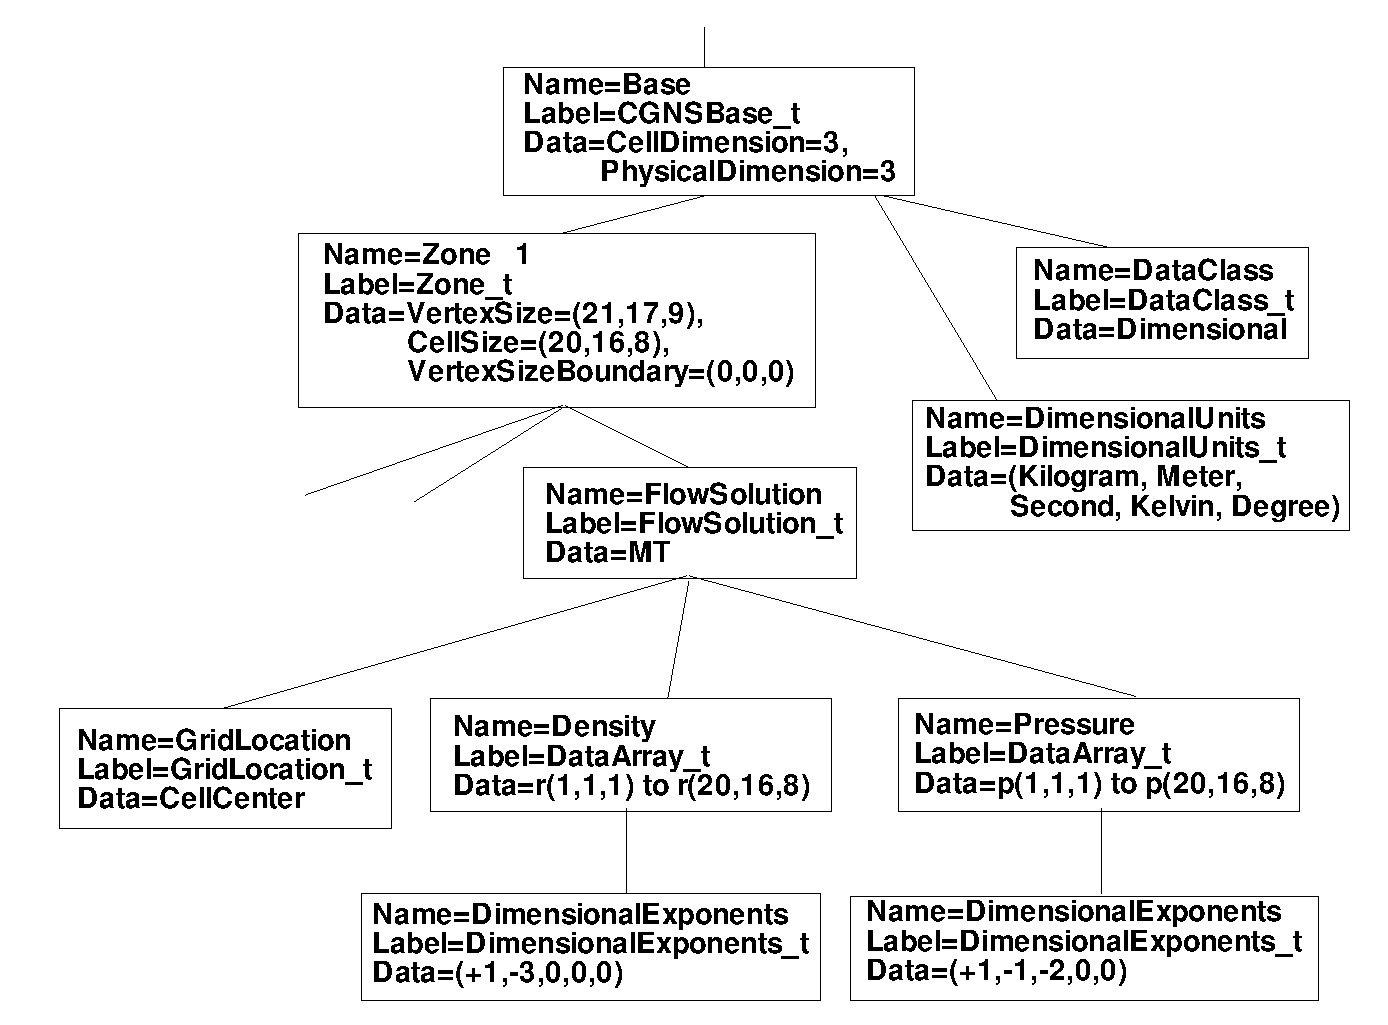
\includegraphics[width=150mm]{figures/tree_dimensional}}}
\caption{Layout of part of a CGNS file for flow solution at cell centers with
dimensional data.}
\label{FIGtree_dimensional}
\end{figure}
%

\subsection{Nondimensional Data} \label{sec:nondimens}

This example is for the relatively common occurrence of CFD
data that is purely nondimensional, for which the
reference state is arbitrary (unknown).  This type is referred
to as {\tt NormalizedByUnknownDimensional}.  Another nondimensional type,
{\tt NormalizedBy\-Dimensional}, for which the data is nondimensional
but the reference state is {\it specifically known}, is not covered
here.

For a {\tt NormalizedByUnknownDimensional} database, the 
{\tt DataClass} is recorded as such, but also a {\tt ReferenceState}
is {\it necessary} to define the nondimensionalizations used. 
(A {\tt ReferenceState\_t} node can be used for any dataset
to indicate the global reference state (such as free stream), as
well as
quantities such as the reference Mach number and Reynolds number.
A {\tt ReferenceState\_t} node was not included in section~\ref{sec:dimens},
but it could have been.)

For the current example, we do not go into detail regarding the 
choices of the items which should populate the reference state for
a {\tt NormalizedByUnknownDimensional} database.  We
simply show in the example some typical choices which very often would
likely be included.  A detailed
discussion of how the data in {\tt ReferenceState\_t} defines the
nondimensionalizations is given in the SIDS document \cite{ALLMARAS}.

--------------------------------------------------------------------

{\tt
\noindent c   WRITE NONDIMENSIONAL INFO
\newline\indent      include 'cgnslib\_f.h'
\newline c   open CGNS file for modify
\newline\indent      call cg\_open\_f('grid.cgns',MODE\_MODIFY,index\_file,ier)
\newline c   we know there is only one base (real working code would check!)
\newline\indent      index\_base=1
\newline c   put DataClass under Base
\newline\indent      call cg\_goto\_f(index\_file,index\_base,ier,'end')
\newline\indent      call cg\_dataclass\_write\_f(NormalizedByUnknownDimensional,ier)
\newline c   put ReferenceState under Base
\newline\indent      call cg\_state\_write\_f('ReferenceQuantities',ier)
\newline c   Go to ReferenceState node, write Mach array and its dataclass
\newline\indent      call cg\_goto\_f(index\_file,index\_base,ier,'ReferenceState\_t',1,
\newline + \indent  'end')
\newline\indent      call cg\_array\_write\_f('Mach',RealSingle,1,1,xmach,ier)
\newline\indent      call cg\_goto\_f(index\_file,index\_base,ier,'ReferenceState\_t',1,
\newline + \indent  'DataArray\_t',1,'end')
\newline\indent      call cg\_dataclass\_write\_f(NondimensionalParameter,ier)
\newline c   Go to ReferenceState node, write Reynolds array and its dataclass
\newline\indent      call cg\_goto\_f(index\_file,index\_base,ier,'ReferenceState\_t',1,
\newline + \indent  'end')
\newline\indent      call cg\_array\_write\_f('Reynolds',RealSingle,1,1,reue,ier)
\newline\indent      call cg\_goto\_f(index\_file,index\_base,ier,'ReferenceState\_t',1,
\newline + \indent  'DataArray\_t',2,'end')
\newline\indent      call cg\_dataclass\_write\_f(NondimensionalParameter,ier)
\newline c   Go to ReferenceState node to write reference quantities:
\newline\indent      call cg\_goto\_f(index\_file,index\_base,ier,'ReferenceState\_t',1,
\newline + \indent  'end')
\newline c   First, write reference quantities that make up Mach and Reynolds:
\newline c   Mach\_Velocity
\newline\indent      call cg\_array\_write\_f('Mach\_Velocity',RealSingle,1,1,xmv,ier)
\newline c   Mach\_VelocitySound
\newline\indent      call cg\_array\_write\_f('Mach\_VelocitySound',RealSingle,
\newline + \indent   1,1,xmc,ier)
\newline c   Reynolds\_Velocity
\newline\indent      call cg\_array\_write\_f('Reynolds\_Velocity',RealSingle,
\newline + \indent   1,1,rev,ier)
\newline c   Reynolds\_Length
\newline\indent      call cg\_array\_write\_f('Reynolds\_Length',RealSingle,
\newline + \indent   1,1,rel,ier)
\newline c   Reynolds\_ViscosityKinematic
\newline\indent      call cg\_array\_write\_f('Reynolds\_ViscosityKinematic',RealSingle,
\newline + \indent   1,1,renu,ier)
\newline c
\newline c   Next, write flow field reference quantities:
\newline c   Density
\newline\indent      call cg\_array\_write\_f('Density',RealSingle,1,1,rho0,ier)
\newline c   Pressure
\newline\indent      call cg\_array\_write\_f('Pressure',RealSingle,1,1,p0,ier)
\newline c   VelocitySound
\newline\indent      call cg\_array\_write\_f('VelocitySound',RealSingle,1,1,c0,ier)
\newline c   ViscosityMolecular
\newline\indent      call cg\_array\_write\_f('ViscosityMolecular',RealSingle,
\newline + \indent   1,1,vm0,ier)
\newline c   LengthReference
\newline\indent      call cg\_array\_write\_f('LengthReference',RealSingle,
\newline + \indent   1,1,xlength0,ier)
\newline c   VelocityX
\newline\indent      call cg\_array\_write\_f('VelocityX',RealSingle,1,1,vx,ier)
\newline c   VelocityY
\newline\indent      call cg\_array\_write\_f('VelocityY',RealSingle,1,1,vy,ier)
\newline c   VelocityZ
\newline\indent      call cg\_array\_write\_f('VelocityZ',RealSingle,1,1,vz,ier)
\newline c   close CGNS file
\newline\indent      call cg\_close\_f(index\_file,ier)
}

--------------------------------------------------------------------

In this case, the only information
added to the CGNS file is at the {\tt CGNSBase\_t} level.
Note that {\tt Mach} and {\tt Reynolds} (which are stored under
{\tt ReferenceState}) are variables that are
known as ``{\tt NondimensionalParameter}''s, so they must
each contain a {\tt DataClass} child node stating this
(the local {\tt DataClass} nodes supersede the overall
{\tt NormalizedByUnknownDimensional} data class that holds for everything else).

The layout of the relevant portion of the resulting CGNS file
from the above example is shown in Fig.~\ref{FIGtree_nondimensional}.
Many of the reference quantities that appear under
{\tt ReferenceState\_t} have been left out of the figure
to conserve space.

% Figure
\begin{figure}[hpbt]
\centerline{{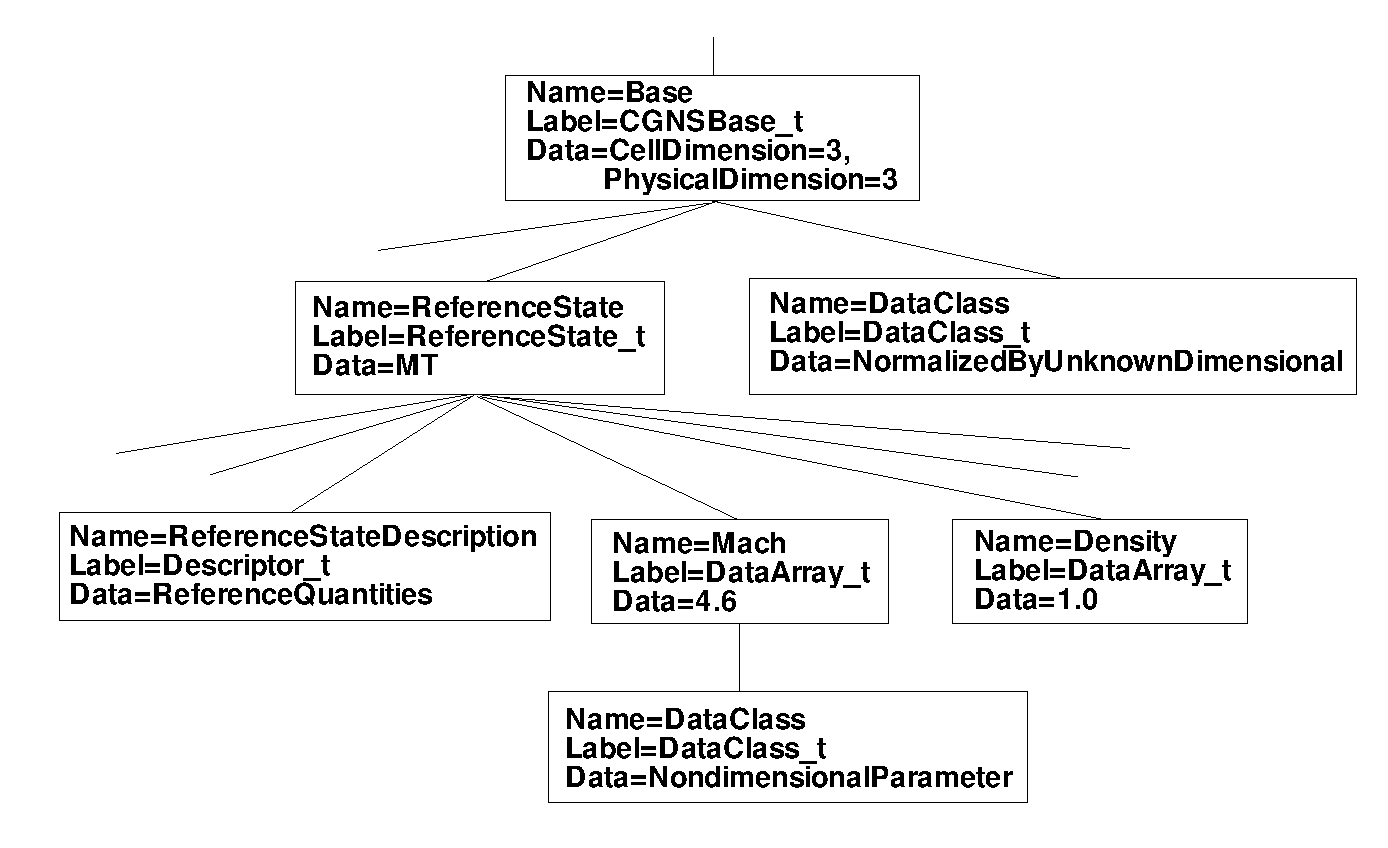
\includegraphics[width=150mm]{figures/tree_nondimensional}}}
\caption{Layout of part of a CGNS file with
purely nondimensional data (reference state unknown).}
\label{FIGtree_nondimensional}
\end{figure}
%

\subsection{Flow Equation Sets} \label{sec:floweqns}

The {\tt FlowEquationSet\_t} node is useful for describing {\it how}
a flow solution was generated.  This is one of the useful
self-descriptive aspects of CGNS that may improve the usefulness and
longevity of a CFD dataset.  For example, under this node, information
such as the following may be recorded:  the flow field was obtained by
solving the thin-layer Navier-Stokes equations (with diffusion only in the
$j$-coordinate direction); the Spalart-Allmaras turbulence
model was employed, and an ideal gas assumption was made with $\gamma=1.4$.

The following FORTRAN code segment writes some of 
the above example flow equation set information
under the {\tt Zone\_t} node from our earlier single-zone structured
grid example from section~\ref{sec:str}.  (Note that 
a {\tt FlowEquationSet\_t} node can also be placed at a higher level,
under the {\tt CGNSBase\_t} node.  The
usual precedence rules apply).

--------------------------------------------------------------------

{\tt
\noindent c   WRITE FLOW EQUATION SET INFO
\newline\indent      include 'cgnslib\_f.h'
\newline c   open CGNS file for modify
\newline\indent      call cg\_open\_f('grid.cgns',MODE\_MODIFY,index\_file,ier)
\newline c   we know there is only one base (real working code would check!)
\newline\indent      index\_base=1
\newline c   we know there is only one zone (real working code would check!)
\newline\indent      index\_zone=1
\newline c   existing file must be 3D structured (real working code would check!)
\newline c   Create 'FlowEquationSet' node under 'Zone\_t'
\newline\indent      call cg\_goto\_f(index\_file,index\_base,ier,'Zone\_t',index\_zone,
\newline + \indent   'end')
\newline c   equation dimension = 3
\newline\indent      ieq\_dim=3
\newline\indent      call cg\_equationset\_write\_f(ieq\_dim,ier)
\newline c
\newline c   Create 'GoverningEquations' node under 'FlowEquationSet'
\newline\indent      call cg\_goto\_f(index\_file,index\_base,ier,'Zone\_t',index\_zone,
\newline + \indent 'FlowEquationSet\_t',1,'end')
\newline\indent      call cg\_governing\_write\_f(NSTurbulent,ier)
\newline c   Create 'DiffusionModel' node under 'GoverningEquations'
\newline\indent      call cg\_goto\_f(index\_file,index\_base,ier,'Zone\_t',index\_zone,
\newline + \indent 'FlowEquationSet\_t',1,'GoverningEquations\_t',1,'end')
\newline\indent      idata(1)=0
\newline\indent      idata(2)=1
\newline\indent      idata(3)=0
\newline\indent      idata(4)=0
\newline\indent      idata(5)=0
\newline\indent      idata(6)=0
\newline\indent      call cg\_diffusion\_write\_f(idata,ier)
\newline c
\newline c   Create 'GasModel' under 'FlowEquationSet'
\newline\indent      call cg\_goto\_f(index\_file,index\_base,ier,'Zone\_t',index\_zone,
\newline + \indent 'FlowEquationSet\_t',1,'end')
\newline\indent      call cg\_model\_write\_f('GasModel\_t',Ideal,ier)
\newline c   Create 'SpecificHeatRatio' under GasModel
\newline\indent      call cg\_goto\_f(index\_file,index\_base,ier,'Zone\_t',index\_zone,
\newline + \indent 'FlowEquationSet\_t',1,'GasModel\_t',1,'end')
\newline\indent      call cg\_array\_write\_f('SpecificHeatRatio',RealSingle,1,1,
\newline + \indent gamma,ier)
\newline c   Create 'DataClass' under 'SpecificHeatRatio'
\newline\indent      call cg\_goto\_f(index\_file,index\_base,ier,'Zone\_t',index\_zone,
\newline + \indent 'FlowEquationSet\_t',1,'GasModel\_t',1,'DataArray\_t',
\newline + \indent 1,'end')
\newline\indent      call cg\_dataclass\_write\_f(NondimensionalParameter,ier)
\newline c   close CGNS file
\newline\indent      call cg\_close\_f(index\_file,ier)
}

--------------------------------------------------------------------

This particular example is specific to a 3-D structured zone.
In an unstructured zone, the use of {\tt DiffusionModel} is not valid.
The layout of the relevant portion of the resulting CGNS file
from the above example is shown in Fig.~\ref{FIGtree_floweqn}.

% Figure
\begin{figure}[hpbt]
\centerline{{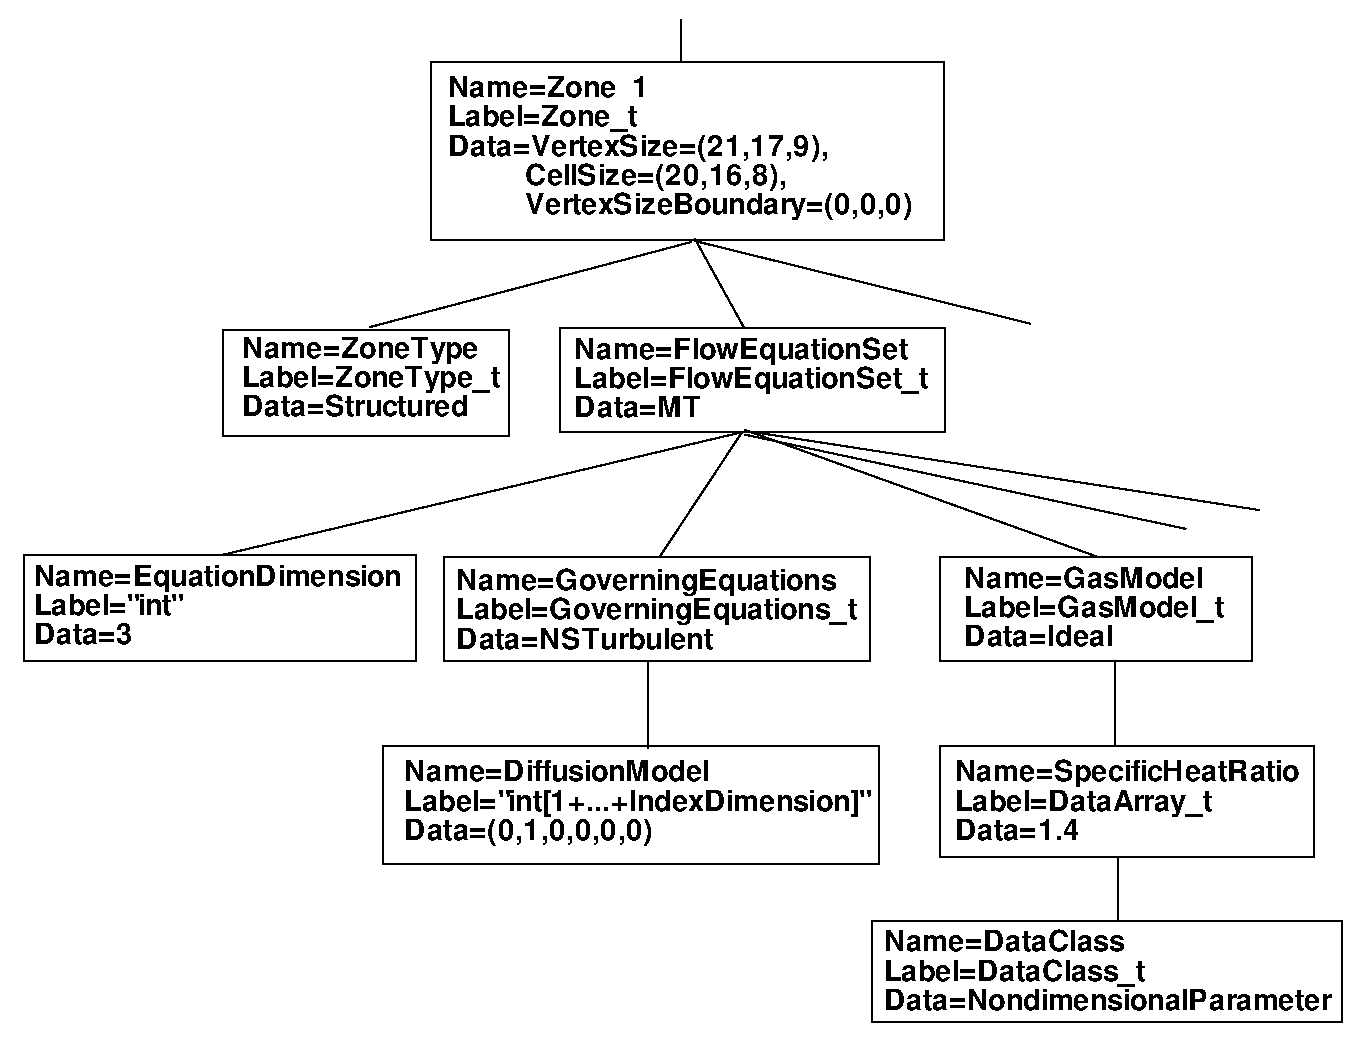
\includegraphics[width=150mm]{figures/tree_floweqn}}}
\caption{Layout of part of a CGNS file with
flow equation set information.}
\label{FIGtree_floweqn}
\end{figure}
%

\subsection{Time-Dependent Data} \label{sec:timeacc}

Time-dependent data (data with multiple flow solutions) can also be stored
in a CGNS file.  Different circumstances may produce
data with multiple flow solutions; for example:

\begin{enumerate}
\item Non-moving grid \label{Item1x}
\item Rigidly-moving grid \label{Item2x}
\item Deforming or changing grid \label{Item3x}
\end{enumerate}

\noindent Each of these may either be
the result of a time-accurate run, or else may simply be
multiple snapshots of a non-time-accurate run as it iterates toward
convergence.

This section gives an example for type~\ref{Item1x} only.  Readers interested
in the two other types should refer to the SIDS document \cite{ALLMARAS}.
For a non-moving grid, the method for storing the multiple flow solutions is relatively simple:
multiple {\tt FlowSolution\_t} nodes,
each with a different name, are placed under each {\tt Zone\_t} node.
However, there also needs to be a mechanism for associating each
{\tt FlowSolution\_t} with a particular time and/or iteration.  This
is accomplished through the use of {\tt BaseIterativeData\_t} (under
{\tt CGNSBase\_t}) and {\tt ZoneIterativeData\_t} (under each {\tt Zone\_t}).
{\tt BaseIterativeData\_t} contains {\tt NumberOfSteps}, the number of times and/or iterations
stored, and their values.  {\tt ZoneIterativeData\_t} contains
{\tt FlowSolutionPointers} as a character data array.  {\tt FlowSolutionPointers}
is dimensioned to be of size {\tt NumberOfSteps}, and contains the {\it names}
of the {\tt FlowSolution\_t} nodes within the current zone that correspond
with the respective times and/or iterations.  Finally, a
{\tt SimulationType\_t} node is placed under {\tt CGNSBase\_t} to
designate what type of simulation (e.g., {\tt TimeAccurate}, {\tt NonTimeAccurate})
produced the data.  (Note:  the {\tt SimulationType\_t} node is not restricted
for use with time-dependent data; {\it any} CGNS dataset can employ it!)

The following FORTRAN code segment writes some of 
the above information, using our
earlier single-zone structured
grid example from section~\ref{sec:str}.  For the purposes of this example,
it is assumed that there are 3 flow solutions from a time-accurate
simulation, to be output as a function of time to the CGNS file.
The variables {\tt r1} and {\tt p1} represent the density and pressure
at time 1, {\tt r2} and {\tt p2} are at time 2, and {\tt r3} and {\tt p3}
are at time 3.

--------------------------------------------------------------------

{\tt
\noindent c   WRITE FLOW SOLUTION TO EXISTING CGNS FILE
\newline\indent      include 'cgnslib\_f.h'
\newline c   open CGNS file for modify
\newline\indent      call cg\_open\_f('grid.cgns',MODE\_MODIFY,index\_file,ier)
\newline c   we know there is only one base (real working code would check!)
\newline\indent      index\_base=1
\newline c   we know there is only one zone (real working code would check!)
\newline\indent      index\_zone=1
\newline c   set up the times corresponding to the 3 solutions to be
\newline c   stored:
\newline\indent      time(1)=10.
\newline\indent      time(2)=20.
\newline\indent      time(3)=50.
\newline c   define 3 different solution names (user can give any names)
\newline\indent      solname(1) = 'FlowSolution1'
\newline\indent      solname(2) = 'FlowSolution2'
\newline\indent      solname(3) = 'FlowSolution3'
\newline c   do loop for the 3 solutions:
\newline\indent      do n=1,3
\newline c   create flow solution node
\newline\indent      call cg\_sol\_write\_f(index\_file,index\_base,index\_zone,solname(n),
\newline + \indent Vertex,index\_flow,ier)
\newline c   write flow solution (user must use SIDS-standard names here)
\newline\indent      if (n .eq. 1) then
\newline\indent      call cg\_field\_write\_f(index\_file,index\_base,index\_zone,index\_flow,
\newline + \indent RealDouble,'Density',r1,index\_field,ier)
\newline\indent      call cg\_field\_write\_f(index\_file,index\_base,index\_zone,index\_flow,
\newline + \indent RealDouble,'Pressure',p1,index\_field,ier)
\newline\indent      else if (n .eq. 2) then
\newline\indent      call cg\_field\_write\_f(index\_file,index\_base,index\_zone,index\_flow,
\newline + \indent RealDouble,'Density',r2,index\_field,ier)
\newline\indent      call cg\_field\_write\_f(index\_file,index\_base,index\_zone,index\_flow,
\newline + \indent RealDouble,'Pressure',p2,index\_field,ier)
\newline\indent      else
\newline\indent      call cg\_field\_write\_f(index\_file,index\_base,index\_zone,index\_flow,
\newline + \indent RealDouble,'Density',r3,index\_field,ier)
\newline\indent      call cg\_field\_write\_f(index\_file,index\_base,index\_zone,index\_flow,
\newline + \indent RealDouble,'Pressure',p3,index\_field,ier)
\newline\indent      end if
\newline\indent      enddo
\newline c   create BaseIterativeData
\newline\indent      nsteps=3
\newline\indent      call cg\_biter\_write\_f(index\_file,index\_base,'TimeIterValues',
\newline + \indent nsteps,ier)
\newline c   go to BaseIterativeData level and write time values
\newline\indent      call cg\_goto\_f(index\_file,index\_base,ier,'BaseIterativeData\_t',
\newline + \indent 1,'end')
\newline\indent      call cg\_array\_write\_f('TimeValues',RealDouble,1,3,time,ier)
\newline c   create ZoneIterativeData
\newline\indent      call cg\_ziter\_write\_f(index\_file,index\_base,index\_zone,
\newline + \indent 'ZoneIterativeData',ier)
\newline c   go to ZoneIterativeData level and give info telling which
\newline c   flow solution corresponds with which time (solname(1) corresponds
\newline c   with time(1), solname(2) with time(2), and solname(3) with time(3))
\newline\indent      call cg\_goto\_f(index\_file,index\_base,ier,'Zone\_t',
\newline + \indent index\_zone,'ZoneIterativeData\_t',1,'end')
\newline\indent      idata(1)=32
\newline\indent      idata(2)=3
\newline\indent      call cg\_array\_write\_f('FlowSolutionPointers',Character,2,idata,
\newline + \indent    solname,ier)
\newline c   add SimulationType
\newline\indent      call cg\_simulation\_type\_write\_f(index\_file,index\_base,
\newline + \indent TimeAccurate,ier)
\newline c   close CGNS file
\newline\indent      call cg\_close\_f(index\_file,ier)
}

--------------------------------------------------------------------

As cautioned for earlier coding snippets, dimensions must be set appropriately
for all variables.  The variable {\tt time} (which is an array dimensioned size 3 in this case)
contains the time values stored under {\tt BaseIterativeData\_t}.
The layout of the resulting CGNS file
from the above example is shown in Fig.~\ref{FIGtree_cartesian_soltime}.
Compare this figure with Fig.~\ref{FIGtree_cartesian_solV}.  To
conserve space, the {\tt GridCoordinates\_t}, {\tt ZoneType\_t}, and
all nodes underneath {\tt FlowSolution\_t} have been left off.

% Figure
\begin{figure}[hpbt]
\centerline{{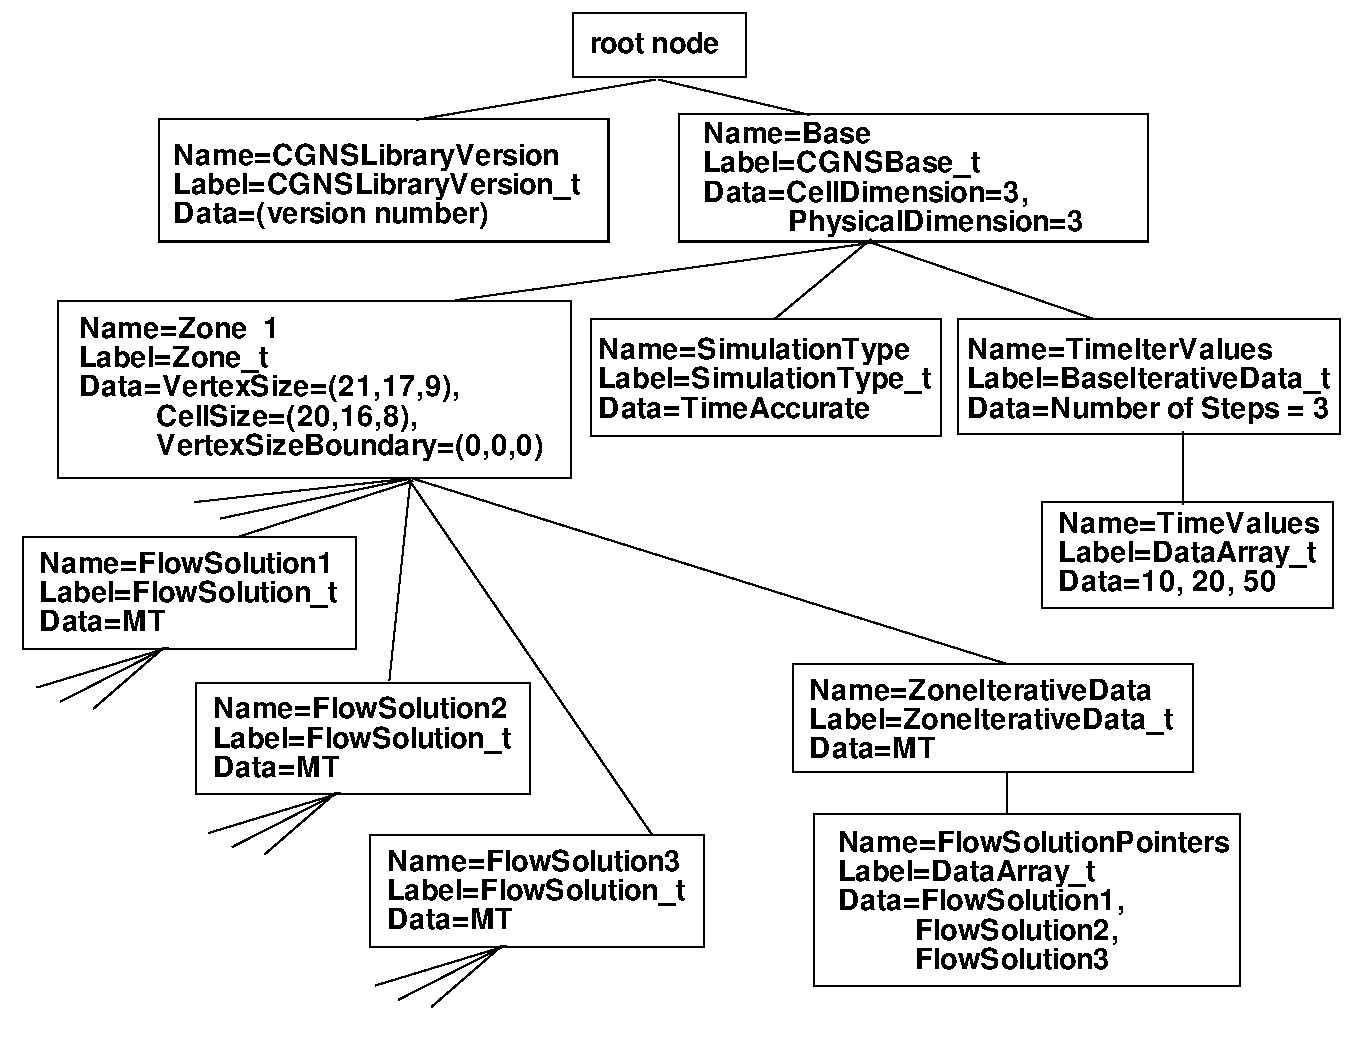
\includegraphics[width=150mm]{figures/tree_cartesian_soltime}}}
\caption{Layout of CGNS file for simple Cartesian
structured grid with multiple time-accurate flow solutions
(non-moving grid coordinates).}
\label{FIGtree_cartesian_soltime}
\end{figure}
%

\subsection{Using Links} \label{sec:links}

A link associates one node to another within a CGNS tree, or even one node
to another in a separate CGNS file altogether.  This can be useful when
there is repeated data; rather than write the same data multiple times,
links can point to the data written only once.

One very important use of links that may be required by many
users is to point to grid coordinates.
This usage comes about in the following way.  Suppose
a user is planning to use a particular grid for multiple cases.  There
are several options for how to store the data.  Among these are:

\begin{enumerate}
\item Keep a copy of the grid with each flow solution in separate CGNS files. \label{Item1}
\item Keep just one CGNS file, with the grid and multiple {\tt FlowSolution\_t}
nodes; each {\tt FlowSolution\_t} node corresponds with a different case. \label{Item2}
\item Keep just one CGNS file, with multiple {\tt CGNSBase\_t} nodes.  The
grid and one flow solution would be stored under one base.
Other bases would each contain a separate flow solution, plus a link
to the grid coordinates in the first base. \label{Item3}
\item Keep one CGNS file with the grid coordinates defined, and store
the flow solution for each case in its own separate CGNS file, with a 
link to the grid coordinates. \label{Item4}
\end{enumerate}

Item~\ref{Item1} is conceptually the most direct, and is certainly the recommended method
in general (this is the way all example CGNS files have been portrayed
so far in this document).  However, if the grid is very large, then this method causes a
lot of storage space to be unnecessarily used to store the same grid
points multiple times.  Item~\ref{Item2} may or may not be a viable option.
If the user is striving to have the CGNS file be completely self-descriptive,
with {\tt ReferenceState} and {\tt FlowEquationSet} 
describing the relevant conditions, then this method
cannot be used if the {\tt ReferenceState} or {\tt FlowEquationSet}
is different between the cases (for example, different Mach numbers,
Reynolds numbers, or angles of attack).
Item~\ref{Item3} removes this restriction.  It uses links to the grid coordinates
within the same file.  
Item~\ref{Item4} is similar to item~\ref{Item3}, except
that the grid coordinates and each flow solution are stored in separate files altogether.

A sample layout showing the relevant portions of two separate CGNS files
for an example of item~\ref{Item4} is shown in Fig.~\ref{FIGtree_link}.
Note that for multiple-zone grids, each zone in FILE 1 in this
example would have a separate link to the appropriate zone's grid
coordinates in FILE 2.

The CGNS API now has the capability to specify links and to query link
information in a CGNS file.
Previously this was only possible by use of the ADF core library
software.
However, when a CGNS file is open for writing and the link creation call
is issued, the link information is merely recorded and the actual link
creation is deferred until the file is written out upon closing it.
Therefore, any attempt to go to a location in a linked file while the
CGNS file is open for writing will fail.
This problem does not exist when a CGNS file is open for modification as
link creation is immediate.

Reading a linked CGNS file presents no difficulties for the API,
because links are ``transparent.''  As long as any separate
linked files keep their name unchanged, and 
maintain the same position (within the Unix-directory)
relative to the parent file, opening the parent
file will automatically access the linked ones.

% Figure
\begin{figure}[hpbt]
\centerline{{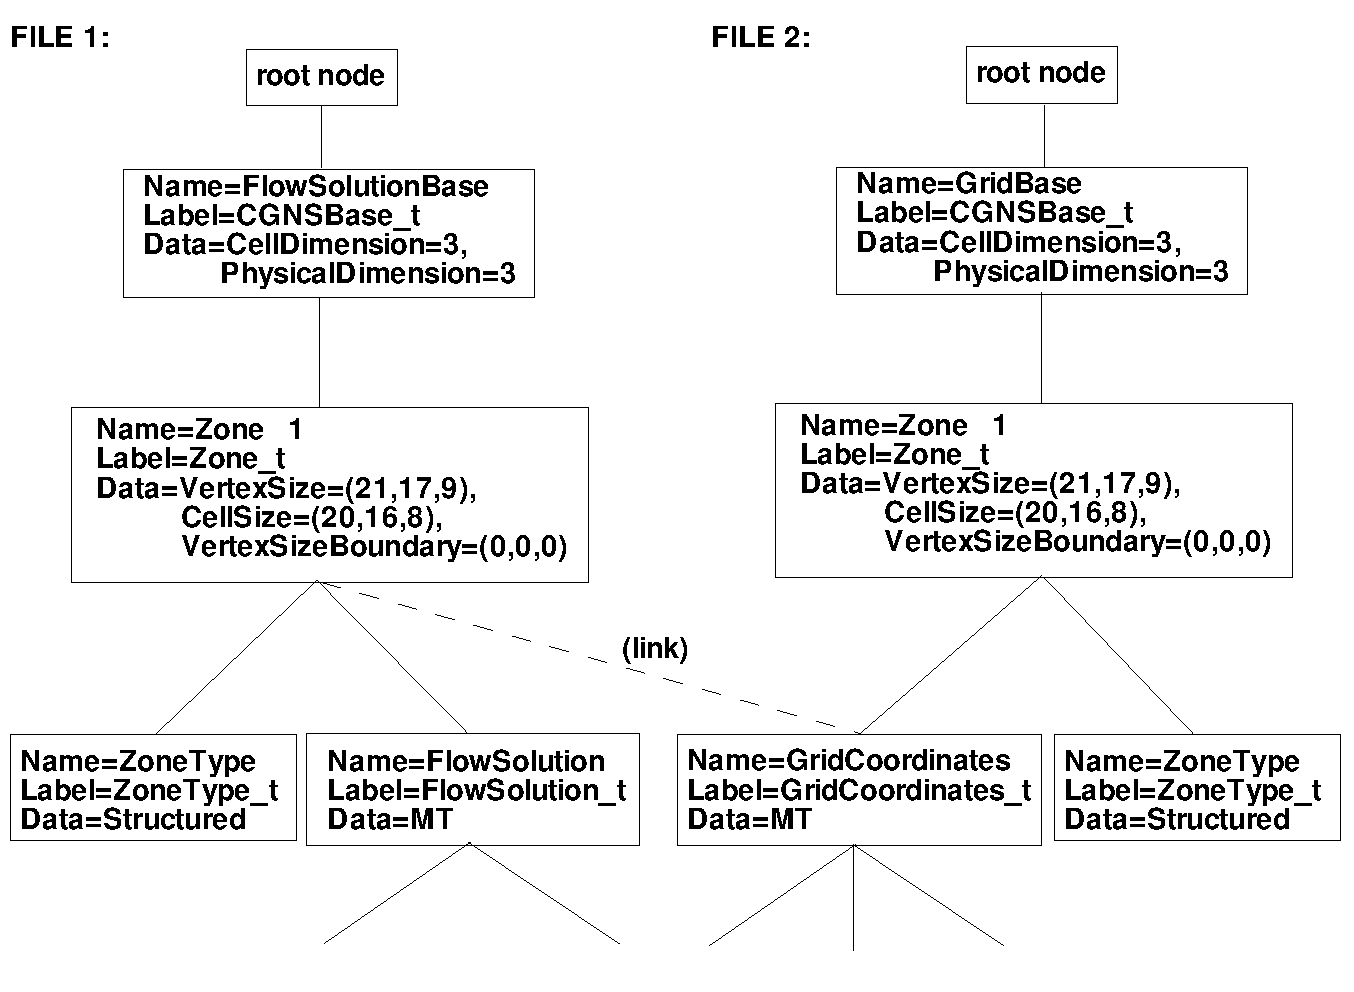
\includegraphics[width=150mm]{figures/tree_link}}}
\caption{Layout of part of two CGNS files with a link
from one to the grid coordinates of the other.}
\label{FIGtree_link}
\end{figure}
%

\newpage
\section{TROUBLESHOOTING} \label{sec:trouble}

\subsection{Handling Errors}

The API has an extensive number of checks for errors, relating
both to illegal usage of ADF as well as relating
to SIDS-noncompliance.
However, it is not guaranteed that
the API will catch all problems prior to reaching the core level.
The list of errors that can arise in the ADF core
routines themselves are not listed here; they
can be found in the file {\tt ADF\_interface.c} under
``Error strings,'' and in the ADF User's Guide \cite{CGNS1}.

If an error occurs, the message given by the ADF or the API
routine should hopefully be descriptive enough to point to the source
of the error.

\subsection{Known Problems}

One known problem that can occur, which is not so much a
problem as it is a restriction, relates to links.  If a user makes
a link from one CGNS file to another, then the linked file
{\it must} have write permission if the user wishes
to open the linking file in {\tt MODE\_MODIFY} or {\tt MODE\_WRITE} mode.
In other words, opening a CGNS file in {\tt MODE\_MODIFY} or {\tt MODE\_WRITE} mode
implies that the {\it entire} CGNS hierarchy, including links (since they are
transparent), is accessible in that mode.  

%One way around this
%restriction is for the user to make a write-permission copy of 
%the linked file.  A second way is to copy the linked file
%into the local file, avoiding the link.  However, this method
%can consume a lot of disk space if the linked file (e.g., GridCoordinates)
%is large and if it is used in concert with many 
%separate local files.
%A third way is to avoid the link by treating the
%two CGNS files as separate entities.  However, this latter method
%in some sense violates the spirit of the SIDS, which presumes (but
%does not require) that
%the GridCoordinates and FlowSolution, for example, are self-contained
%in a single CGNS hierarchy.

\newpage
\section{FREQUENTLY ASKED QUESTIONS} \label{sec:FAQ}

~

Q:  Does CGNS support solution array names that are not listed in the SIDS?

A:  You can use any data-name that you want for solution arrays.  However,
if you create a new name not listed in the SIDS, it may not be understood
by other applications reading your file.

----------------------------

Q:  What is a {\tt Family} in CGNS?

A:  The families are used to link the mesh to the geometry.  The data
structure Family\_t is optional and can be used to define the geometry
of boundary patches by referencing CAD entities.  In turn, mesh
patches can reference family, so we get:  mesh -$>$ family -$>$ geometry.

----------------------------

Q:  What are {\tt DiscreteData\_t} and {\tt IntegralData\_t} used for?

A: {\tt DiscreteData\_t} can be used to store field data that is not
typically considered part of the flow solution {\tt FlowSolution\_t}.
{\tt IntegralData\_t} can be used to store generic global or integral
data (a single integer or floating point number is allowed in each {\tt
DataArray\_t} node under {\tt IntegralData\_t}).

----------------------------

Q:  What are some good programming practices that will help me avoid
problems when implementing CGNS in my code?

A:  The usual good programming standards apply:  
use plenty of comments, use logical indentation to make the code more
readable, etc.  In addition, the API returns an error code from
each of its calls; it is a good idea to check this regularly and
gracefully exit the program with an error message when it is not
zero.  In FORTRAN, you can use:

\indent {\tt if (ier .ne. 0) call cg\_error\_exit\_f}

----------------------------

Q:  How can I look at what is in a CGNS file?

A:  The utility \underbar{ADFviewer} is the best way to look at a CGNS
file.  This utility allows you to access any node in the file using
a Windows-like collapsible node tree. Nodes and data may be added,
deleted, and modified.
It also has translator capabilities and a crude built-in compliance checker.

----------------------------

Q:  How can I tell if I have created a truly SIDS-compliant CGNS file?

A:  It is currently very difficult to {\it guarantee} that a user has created
a SIDS-compliant CGNS file, that others can read and understand.  But because
the API (mid-level-library) has many checks for non-compliance, it is
much more difficult for you to make a mistake when using it
than if you utilize ADF (core-level) calls.
Also, as mentioned above,
the \underbar{adfviewer} utility has a crude built-in compliance checker.

----------------------------

Q:  How do I write data sets associated with boundary conditions?

A:  Writing data sets under boundary conditions is following the
    ``fully SIDS-compliant BC implementation'' rather than the ``lowest
    level BC implementation''.
    (See Fig.~\ref{FIGbc} in Appendix~\ref{sec:sidsoverview}).
    In order to do this using the Mid-Level Library, take the following
    steps:
    \begin{enumerate}
    \item Use \texttt{cg\_boco\_write} to create each \texttt{BC\_t}
          node and its associated \texttt{BCType} and boundary condition region.
          (This also creates the top level \texttt{ZoneBC\_t} node if it
          does not already exist.
          Note that only one \texttt{ZoneBC\_t} node may exist under any
          given \texttt{Zone\_t} node.)
          This is the only step necessary to achieve the ``lowest level
          BC implementation.''
    \item Use \texttt{cg\_dataset\_write} to create each
          \texttt{BCDataSet\_t} node and its associated
          \texttt{BCTypeSimple} under the desired \texttt{BC\_t} node.
    \item Use \texttt{cg\_bcdata\_write} to create each
          \texttt{BCData\_t} node (of either type \texttt{Dirichlet}
          or \texttt{Neumann}) under the desired \texttt{BCDataSet\_t}
          node.
    \item Use \texttt{cg\_goto} to ``go to'' the appropriate
          \texttt{BCData\_t} node.
    \item Use \texttt{cg\_array\_write} to write the desired data.
    \end{enumerate}

\newpage
\appendix
%\renewcommand{\thesection}{}
%\section{\bf APPENDIX A:  THE ADFEDIT UTILITY}
\app{EXAMPLE COMPUTER CODES} \label{sec:codes}

The following computer codes are complete, workable versions of the codes
mentioned in the text of this User's Guide (plus some that are
not mentioned).  They can be obtained from the CGNS site at SourceForge
(\underbar{sourceforge.net/projects/cgns}).
They read and write very simple example CGNS files, in order to help
the user understand the CGNS concepts as well as the usage of the API calls.
Instructions for compiling them on LINUX systems is contained in comment
lines in each program. 
The following codes are written in both
FORTRAN and C.

Note that these programs are very unsophisticated, purposefully
for ease of readability.  Real working codes would be written more
generally, with more checks, and would {\it not} be as hardwired for
particular cases. The codes are listed here by corresponding section.

~\newline
\underbar{STRUCTURED GRID}

\noindent Section~\ref{sec:singlegrid}:

\begin{tabular}{ | l | l | }
\hline
write\_grid\_str.f         & writes grid \\ \hline
write\_grid\_str.c         & writes grid (C-program example) \\ \hline
read\_grid\_str.f          & reads grid \\ \hline
\end{tabular}

~\newline
Section~\ref{sec:flowsoln}:

\begin{tabular}{ | l | l | }
\hline
write\_flowvert\_str.f     & writes vertex-based flow solution \\ \hline
read\_flowvert\_str.f      & reads vertex-based flow solution \\ \hline
write\_flowcent\_str.f     & writes cell centered flow solution \\ \hline
read\_flowcent\_str.f      & reads cell centered flow solution \\ \hline
write\_flowcentrind\_str.f & writes cell centered flow solution with rind cells \\ \hline
read\_flowcentrind\_str.f  & reads cell centered flow solution with rind cells \\ \hline
\end{tabular}

~\newline
Section~\ref{sec:bcstruct}:

\begin{tabular}{ | l | l | }
\hline
write\_bc\_str.f           & writes PointRange boundary condition patches \\ \hline
read\_bc\_str.f            & reads PointRange boundary condition patches \\ \hline
write\_bcpnts\_str.f       & writes PointList boundary condition patches \\ \hline
read\_bcpnts\_str.f        & reads PointList boundary condition patches \\ \hline
\end{tabular}

~\newline
Section~\ref{sec:str1to1}:

\begin{tabular}{ | l | l | }
\hline
write\_grid2zn\_str.f      & writes 2-zone grid \\ \hline
read\_grid2zn\_str.f       & reads 2-zone grid \\ \hline
write\_con2zn\_str.f       & writes 1-to-1 connectivity for 2-zone example \\ \hline
read\_con2zn\_str.f        & reads 1-to-1 connectivity for 2-zone example \\ \hline
write\_con2zn\_genrl\_str.f & writes general 1-to-1 connectivity for 2-zone example \\ \hline
read\_con2zn\_genrl\_str.f  & reads general 1-to-1 connectivity for 2-zone example \\ \hline
\end{tabular}

~\newline

~\newline
\underbar{UNSTRUCTURED GRID}

\noindent Section~\ref{sec:unstrgrid}:

\begin{tabular}{ | l | l | }
\hline
write\_grid\_unst.f        & writes grid \\ \hline
read\_grid\_unst.f         & reads grid \\ \hline
\end{tabular}

~\newline
Section~\ref{sec:unstrflow}:

\begin{tabular}{ | l | l | }
\hline
write\_flowvert\_unst.f    & writes vertex-based flow solution \\ \hline
read\_flowvert\_unst.f     & reads vertex-based flow solution \\ \hline
\end{tabular}

~\newline
Section~\ref{sec:bcunstr}:

\begin{tabular}{ | l | l | }
\hline
write\_bcpnts\_unst.f      & writes PointList boundary condition patches (FaceCenter) \\ \hline
read\_bcpnts\_unst.f       & reads PointList boundary condition patches (FaceCenter) \\ \hline
\end{tabular}

~\newline
\underbar{GENERAL}

\noindent Section~\ref{sec:converge}:

\begin{tabular}{ | l | l | }
\hline
write\_convergence.f      & writes convergence history \\ \hline
read\_convergence.f       & reads convergence history \\ \hline
\end{tabular}

~\newline
Section~\ref{sec:descript}:

\begin{tabular}{ | l | l | }
\hline
write\_descriptor.f       & writes descriptor node under CGNSBase\_t \\ \hline
read\_descriptor.f        & reads descriptor node under CGNSBase\_t \\ \hline
\end{tabular}

~\newline
Section~\ref{sec:dimens}:

\begin{tabular}{ | l | l | }
\hline
write\_dimensional.f      & writes dimensional data to an existing grid + flow solution \\ \hline
read\_dimensional.f       & reads dimensional data from an existing grid + flow solution \\ \hline
\end{tabular}

~\newline
Section~\ref{sec:nondimens}:

\begin{tabular}{ | l | l | }
\hline
write\_nondimensional.f   & writes nondimensional data to an existing CGNS file \\ \hline
read\_nondimensional.f    & reads nondimensional data from an existing CGNS file \\ \hline
\end{tabular}

~\newline
Section~\ref{sec:floweqns}:

\begin{tabular}{ | l | l | }
\hline
write\_floweqn\_str.f     & writes flow equation information for structured example \\ \hline
read\_floweqn\_str.f      & reads flow equation information for structured example \\ \hline
\end{tabular}

~\newline
Section~\ref{sec:timeacc}:

\begin{tabular}{ | l | l | }
\hline
write\_timevert\_str.f     & writes time-dependent flow soln (as Vertex) for structured example \\ \hline
read\_timevert\_str.f      & reads time-dependent flow soln (as Vertex) for structured example \\ \hline
\end{tabular}

\newpage
%\appendix
%\renewcommand{\thesection}{}
%\section{\bf APPENDIX C:  OVERVIEW OF THE SIDS}
\app{OVERVIEW OF THE SIDS}  \label{sec:sidsoverview}

%\renewcommand{\thesubsection}{}
%\subsection{\bf C.1  The Big Picture} \label{sec:bigp}
\subapp{The Big Picture} \label{sec:bigp}

As mentioned in the Introduction, a 
CGNS file is organized into a set of ``nodes'' in a tree-like
structure, in much the same way as directories are
organized in the UNIX environment.
Each node is identified by both a label and a name.
Most node {\it labels} are given by a series of characters 
followed by ``\_t''.  There are generally very strict rules
governing the labeling conventions in a CGNS file.  Node {\it names} 
are sometimes user-defined, but sometimes must also follow 
strict naming conventions.  The label identifies
a ``{\it type}.''  For example, {\tt Zone\_t} identifies a Zone-type
node, and {\tt DataArray\_t} identifies a type of node that contains
a data array.  The name identifies a specific instance of
the particular node type.  For example, {\tt Density} is the name of
a node of type {\tt DataArray\_t} that contains an array of densities.

As you become more familiar with how CGNS files are
organized, you will notice that,
generally, the higher you are in the CGNS hierarchy, the more
important the label is (names tend to be user-defined); whereas
the lower you are in the hierarchy, the more important the
name is.  This convention arises because at the higher levels,
the broader categories are established, and are used to determine
``where to go'' in the hierarchy.   At the lower levels, the category becomes
less important because this is the region where you are
searching for specific items.

Throughout the remainder of this
first section, we will primarily be referring to the nodes by their
{\it label}, because we are focusing on the ``big picture.''
In later sections, as we get into specific examples,
both names and labels will be referred to.

It is important to note at this point that the SIDS document
specifies the layout of the CGNS file, in terms of parents
and children.  However, when a given piece of information is
listed as being ``under'' a node, there are actually two possibilities:
the information can be stored {\it as data \underbar{in} the current node},
or it can be stored {\it as data \underbar{in or under} a separate child node}.
This distinction is illustrated in Fig.~\ref{FIGdataorchild}.  
The SIDS-to-ADF
mapping document \cite{CGNS2} determines which of the two
possibilities are used for each situation, and must always be
consulted along with the SIDS document.  (Note there is also a SIDS-to-HDF5
document available.) Throughout the remainder
of this appendix, the location of information (whether
as data or as a separate child node) will always be explicitly
specified, according to the SIDS-to-ADF mapping document.

% Figure
\begin{figure}[hpbt]
\centerline{{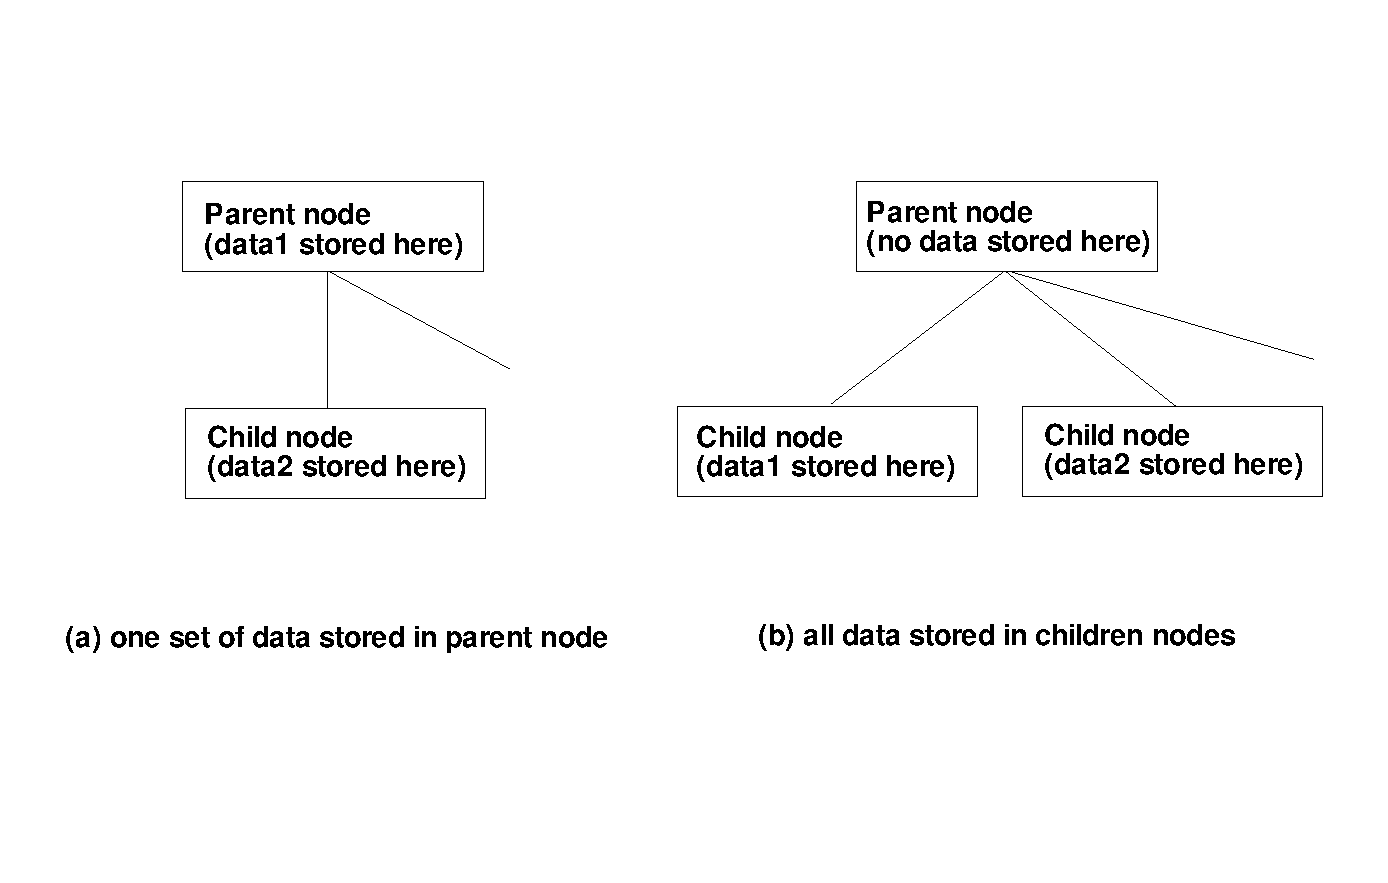
\includegraphics[width=150mm]{figures/dataorchild}}}
\caption{Two possible treatments of a parent node with sets
of data ``under'' it.}
\label{FIGdataorchild}
\end{figure}
%

The remainder of this appendix attempts to summarize the most
important and most commonly-used aspects of the SIDS.  It does not
cover all possible nodes or situations.  It is intended as a 
general overview only.  It is also likely
that future extensions to the SIDS will add additional capabilities
beyond what we cover here.

The top, or entry-level, of the CGNS file is always what is 
referred to as the ``root node.''  Children to be found
directly under this node are the node {\tt CGNSLibraryVersion\_t} and
one or more {\tt CGNSBase\_t} nodes.  The {\tt CGNSLibraryVersion\_t} node
has, as its data, the version (release) number
of the CGNS standard as defined by the SIDS.
The {\tt CGNSBase\_t} node represents the top level for a given 
database, or ``case.''
Most CGNS files will only have one {\tt CGNSBase\_t} node, although
the SIDS allows for any number in order to remain extensible
and to allow for the possibility of having more than one
``case'' in a single file.  Here, the definition of ``case''
is left open.  For the remainder of this appendix, we assume that
there is only one {\tt CGNSBase\_t} node within a given CGNS file.

The {\tt CGNSBase\_t} node may have, as its children, the following
nodes:  {\tt Zone\_t}, 
\newline {\tt ConvergenceHistory\_t}, {\tt BaseIterativeData\_t}, 
{\tt SimulationType\_t}, {\tt Family\_t}, {\tt IntegralData\_t}, 
{\tt DataClass\_t}, {\tt FlowEquationSet\_t}, 
{\tt DimensionalUnits\_t}, {\tt ReferenceState\_t},
{\tt Axisymmetry\_t}, {\tt RotatingCoordinates\_t}, {\tt Gravity\_t},
{\tt UserDefinedData\_t}, and {\tt Descriptor\_t}.  

The {\tt Zone\_t} node gives information about a particular zone of
the grid; most of the data in the CGNS file is usually found 
under this node.  Any 
number of {\tt Zone\_t} nodes is allowed at this level.  Its children will 
be described in greater detail below.  {\tt ConvergenceHistory\_t}
contains solution history information typically output by many
CFD codes, such as residual, lift, drag, etc. as a function of
iteration number.  By convention, its name is
{\tt GlobalConvergenceHistory}.  A {\tt ConvergenceHistory\_t} node can exist
under the {\tt Zone\_t} node as well, but there, its name is by convention 
{\tt ZoneConvergenceHistory}.  {\tt BaseIterativeData\_t}
stores information relating to the times and/or iteration numbers
for a database in which flow solutions and/or grids at 
multiple times are stored.  {\tt SimulationType\_t}
describes the type of simulation stored (i.e., {\tt TimeAccurate} or 
{\tt NonTimeAccurate}).  {\tt Family\_t} is generally used
to tie the grid to geometric CAD data, or to link certain
entities together as a common part (e.g., ``wing,'' ``strut,''
etc.).  Any number of {\tt Family\_t} nodes is allowed.
{\tt Axisymmetry\_t}, {\tt RotatingCoordinates\_t}, and {\tt Gravity\_t}
are used for specific situations; details can be found in the SIDS.

The remaining nodes allowed under {\tt CGNSBase\_t} are somewhat
more generic, and can exist at other levels in the hierarchy
beside this one.  They are briefly described here.
{\tt IntegralData\_t} is a ``catch-all'' node for storing any 
desired sets of generic data.  Any number of {\tt IntegralData\_t}
nodes is allowed at this level. 
{\tt DataClass\_t} (which, by convention, has the name {\tt DataClass})
indicates the form that the data in the {\tt CGNSBase\_t} is
stored, for example:  {\tt Dimensional}, {\tt NormalizedByDimensional},
or {\tt NormalizedByUnknownDimensional}. 
{\tt FlowEquationSet\_t} 
(which, by convention, has the name {\tt FlowEquationSet})
defines the equations used in the CFD
simulation.  {\tt DimensionalUnits\_t} (which, by convention, has the name 
{\tt DimensionalUnits})
defines the dimensional units used (if any).  {\tt ReferenceState\_t}
(which, by convention, has the name {\tt ReferenceState})
defines a reference state.  This node is where quantities such
as Reynolds number, Mach number, and other reference quantities
that define the flow field conditions and/or the 
nondimensionalizations are stored.  {\tt UserDefinedData\_t} is used to store
user-defined data that is (by definition) not part of the SIDS standard.
Finally, {\tt Descriptor\_t}
is used to store descriptor strings. 
Any number of {\tt Descriptor\_t} nodes is allowed at this level.

The data stored within the {\tt CGNSBase\_t} node itself are the 
{\tt CellDimension} and the {\tt PhysicalDimension}.  The {\tt CellDimension}
is the dimensionality of the cells in the mesh
(e.g., 3 for volume cell, 2 for face cell).  The {\tt PhysicalDimension}
is the number of coordinates required to
define a node position (e.g., 1 for 1-D, 2 for 2-D, 3 for 3-D).
The index dimension, which is the number of different indices required
to reference a node (e.g., 1=i, 2=i,j, 3=i,j,k), is not stored,
but can be determined for each zone
based on its type ({\tt Structured} or {\tt Unstructured}).  If
{\tt Structured}, the index dimension is the same as {\tt CellDimension}.
If {\tt Unstructured}, the index dimension is 1.

Much information can be stored under {\tt Zone\_t}.  Because this is
an overview, we do not go through it all here.  Instead, we only
highlight the features that most users are likely to use. 
{\tt ZoneType\_t} (which, by convention, has the name {\tt ZoneType})
stores the name {\tt Structured} or {\tt Unstructured}.
{\tt GridCoordinates\_t} is the parent node of the grid coordinates 
arrays, such as
{\tt CoordinateX}, {\tt CoordinateY}, 
and {\tt CoordinateZ}.  
Any number of {\tt GridCoordinates\_t} nodes are
allowed at this level (to handle the case of deforming
grids).  By convention, the original grid coordinates
has the name {\tt GridCoordinates}.
{\tt FlowSolution\_t} stores under it nodes which contain the flow
solution; for example, {\tt Density}, {\tt VelocityX}, 
{\tt VelocityY},
{\tt VelocityZ}, and {\tt Pressure}.  It also gives the location
at which the solution is stored (e.g., {\tt CellCenter}, {\tt Vertex}), and
includes the possibility for including {\tt Rind} (ghost cell or ghost point) information.
Any number of {\tt FlowSolution\_t} nodes are
allowed at this level.  The {\tt Elements\_t} data structure holds
unstructured element data such as connectivity, neighbors,
etc.  Any number of 
{\tt Elements\_t} nodes are allowed at this level.
{\tt ZoneIterativeData\_t} stores information necessary
for a database in which flow solutions at multiple times are stored.
Other important nodes under {\tt Zone\_t} are {\tt ZoneBC\_t}
(which, by convention, has the name {\tt ZoneBC})
and {\tt ZoneGridConnectivity\_t} (which, by convention, has the name 
{\tt ZoneGridConnectivity}).  These store the boundary conditions and
the grid connectivity information, respectively.
More will be said about these nodes later.

The data stored within the {\tt Zone\_t} node itself are the
{\tt VertexSize}, the {\tt CellSize}, and the {\tt VertexSizeBoundary}.  These
are dimensioned by the index dimension, and give the number
of vertices, the number of cells, and the number of boundary
vertices (used for sorted elements in unstructured zones only),
respectively.

An important point to note here is that the API sorts the {\tt Zone\_t}
nodes alphanumerically according to their {\it name} when
it reads them.  This
was deemed necessary because most CFD codes currently perform
operations on the zones of multiple-zone grids in a certain order.
To duplicate existing non-CGNS applications, it is 
necessary to insure that zones can be read in the desired
sequence.  (ADF does not necessarily retrieve data in the same 
order in which it was stored, so the API reader for zones was
built to do this.)  Hence, when {\it naming} zones, the user should
make sure they are named alphanumerically (if an ordering is
desired).

For example, the naming convention {\tt ZoneN}, where N is the zone
number, is alphanumeric only up to {\tt Zone9}.  {\tt Zone10} through
{\tt Zone19} would get sorted between {\tt Zone1} and {\tt Zone2}, and so on.
Spaces are allowed in names, so {\tt Zone~~N}, with two spaces, 
(e.g., {\tt Zone~~1}, {\tt Zone~~2},...
{\tt Zone~99}, {\tt Zone100},...) is alphanumeric up to {\tt Zone999}.  Other
zone naming conventions are certainly possible, and are completely
up to the user to define appropriately.

A summary graphic of the overall layout of a typical CGNS file 
is given in Fig.~\ref{FIGoverviewSTR}.  
% Figure
\begin{figure}[hpbt]
\centerline{{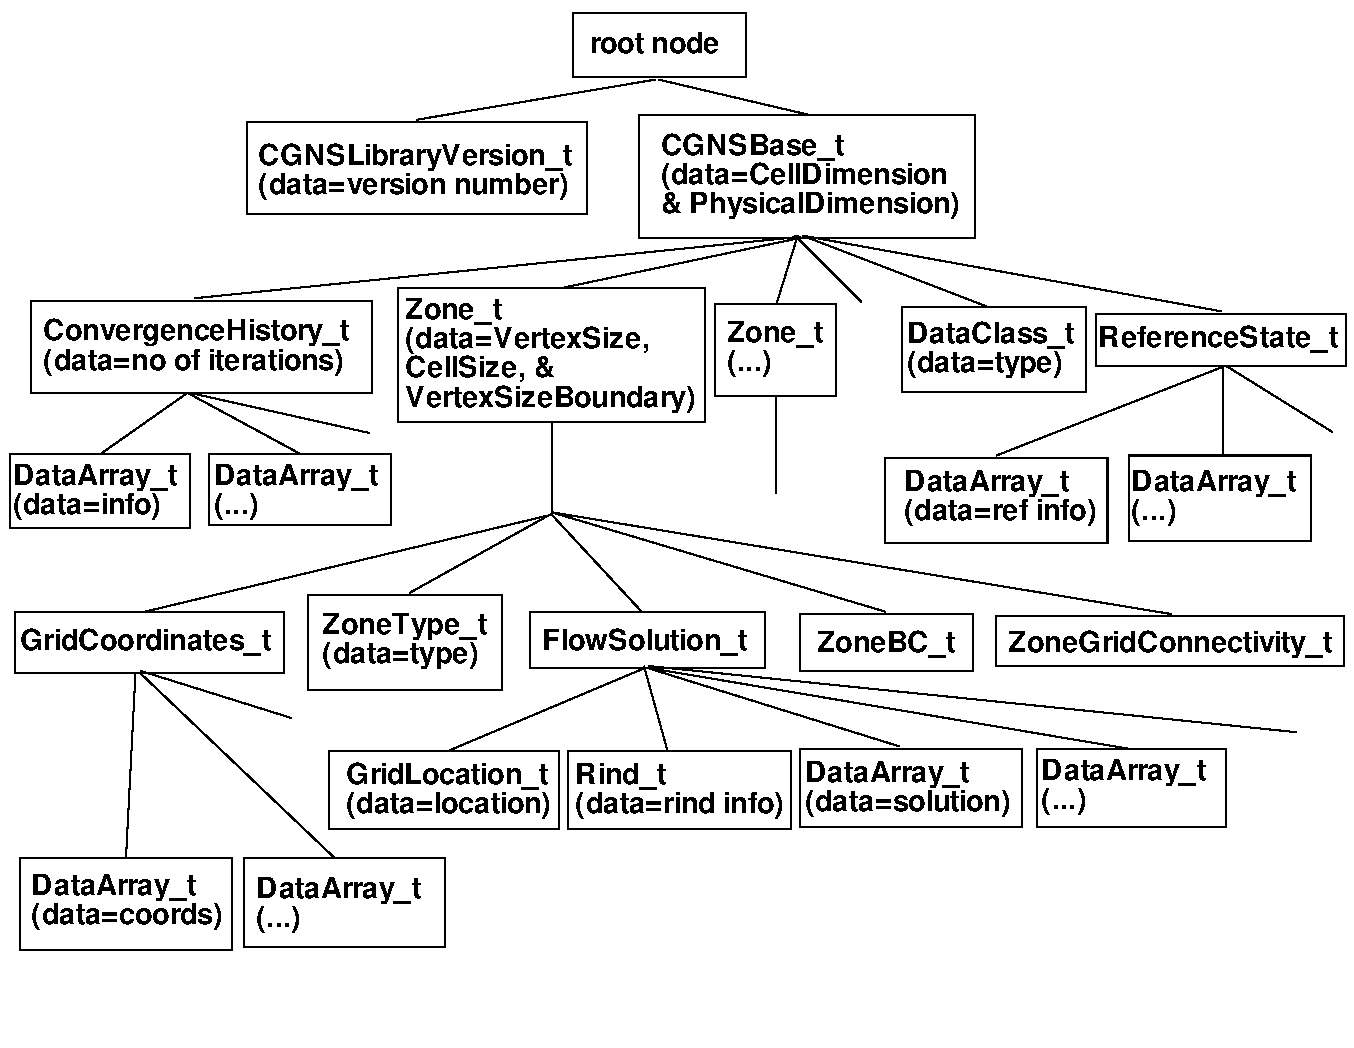
\includegraphics[width=150mm]{figures/overviewSTR}}}
\caption{Hierarchical structure of a typical CGNS file (structured
grid type).}
\label{FIGoverviewSTR}
\end{figure}
%
This figure shows the hierarchical data structure,
and the relative locations of the nodes.  It also indicates
(informally) what data, if any, is stored {\it within} each node.
Note that all possible nodes are {\it not}
included here.  In particular, note that {\tt Elements\_t} nodes are
not shown under {\tt Zone\_t}; 
\underbar{the {\tt Elements\_t} nodes would be present
for an unstructured zone}.  
Also note that nodes that occur
under {\tt ZoneBC\_t} and {\tt ZoneGridConnectivity\_t} have been omitted;
these will also be covered below.  Optional nodes such as 
{\tt SimulationType\_t} (under {\tt CGNSBase\_t}) are not included.  And finally, note that
multiple {\tt GridCoordinates\_t} and {\tt FlowSolution\_t} nodes are allowed, 
but we show in the figure only one of each.  
Multiple {\tt FlowSolution\_t} nodes are usually only used in
the situation when multiple times of time-accurate data are
stored, and multiple {\tt GridCoordinates\_t} nodes are used
for deforming grids.

~

%\renewcommand{\thesubsection}{}
%\subsection{\bf C.2  Implementation at the Lower Levels of the Hierarchy}
\subapp{Implementation at the Lower Levels of the Hierarchy}

Most of the actual data is at the lower levels of the CGNS
hierarchy.  We do not go into great detail here; the examples 
in the main body of this document serve as instruction for this.
However, there are several general items of importance 
related to the storage of data that are appropriate to mention
here.

Many specific items, variables, and conditions that relate to CFD
data are specified in the SIDS.  These are standardized {\it names} 
that must be used in order that other users will understand
what is in your CGNS file.  For example, the static density must
be called {\tt Density}.  Any other name may not be recognized by other
users.  In fact, if another application code expects ``{\tt Density},'' but
you name it ``{\tt density}'' (lower case ``d''), then chances are the
other code's search will fail.

Naturally, the items listed in the SIDS
cannot cover all possible items required by users.
Hence, the SIDS allows for the use of the 
type {\tt UserDefinedData\_t} for any special type not covered.
For example, there are currently only a limited number of
defined names for turbulence models in the SIDS (e.g.,
{\tt OneEquation\_SpalartAllmaras}).  As everyone knows, there
are a {\it huge} number of turbulence models and turbulence model
variants that exist, so that the SIDS cannot hope to
define standardized names for all of them.  The type {\tt UserDefinedData\_t}
covers this situation.

When {\tt UserDefinedData\_t} is used, however, the user runs the risk
that others will be unable to interpret the CGNS file.  We 
therefore recommend
that whenever a {\tt UserDefinedData\_t} type is unavoidable, the user also include
a companion {\tt Descriptor\_t} node to specify what was done.

It is possible that, if certain items are found to be used
more heavily as time goes on, that standardized names may be created and added
to the SIDS in the future.

~

%\renewcommand{\thesubsection}{}
%\subsection{\bf C.3  Boundary Conditions}
\subapp{Boundary Conditions}

The boundary conditions hierarchical structure in CGNS can appear
to be somewhat daunting at first.  Because the CGNS team decided
to make the boundary condition information as descriptive as possible
and easily extensible to complex situations, there are many
layers possible in the hierarchy, and the usage rules can
become complex.

However, the SIDS allows for use of simplified versions of the
{\tt ZoneBC\_t} node, which are easier to understand and adopt.
Essentially, the simplified versions ``cut off'' the hierarchy
at a higher level than the full-blown 
SIDS boundary condition description.  The
implication of this is that application codes that use
a simplified version must interpret what is meant by each 
particular boundary condition type, without the help of the CGNS file.

For example, the boundary condition 
type {\tt BCFarfield} indicates a boundary condition
applied to a far field boundary.  Most CFD codes have this type,
which performs different functions depending upon whether the
local flow field is inflow or outflow, subsonic or supersonic.
The full-blown SIDS description of {\tt BCFarfield} attempts to
describe in some detail the methodology involved in this boundary
condition.  However, if the user chooses to use the minimal ``cut off''
version, the only information regarding the function of the
boundary condition that is stored in the CGNS file is the
{\it name} {\tt BCFarfield}.  An application code must determine from this name
alone what is meant.

%Boundary conditions can be completely unambiguous 
%(e.g., the name BCSymmetryPlane unambiguously defines a boundary
%condition), or they can be somewhat generic.  For example,
%even if one were to use the full-blown SIDS description
%of BCFarfield, there is still some ambiguity as to precisely
%{\it how} a code might choose to implement the details.  Therefore,
%one might argue that there is no point to defining a generic boundary
%condition below the level of its generic name.  However,
%having these additional levels available allows for future
%extensibility of CGNS to handle currently-unforeseen situations.

% Figure
\begin{figure}[hpbt]
\centerline{{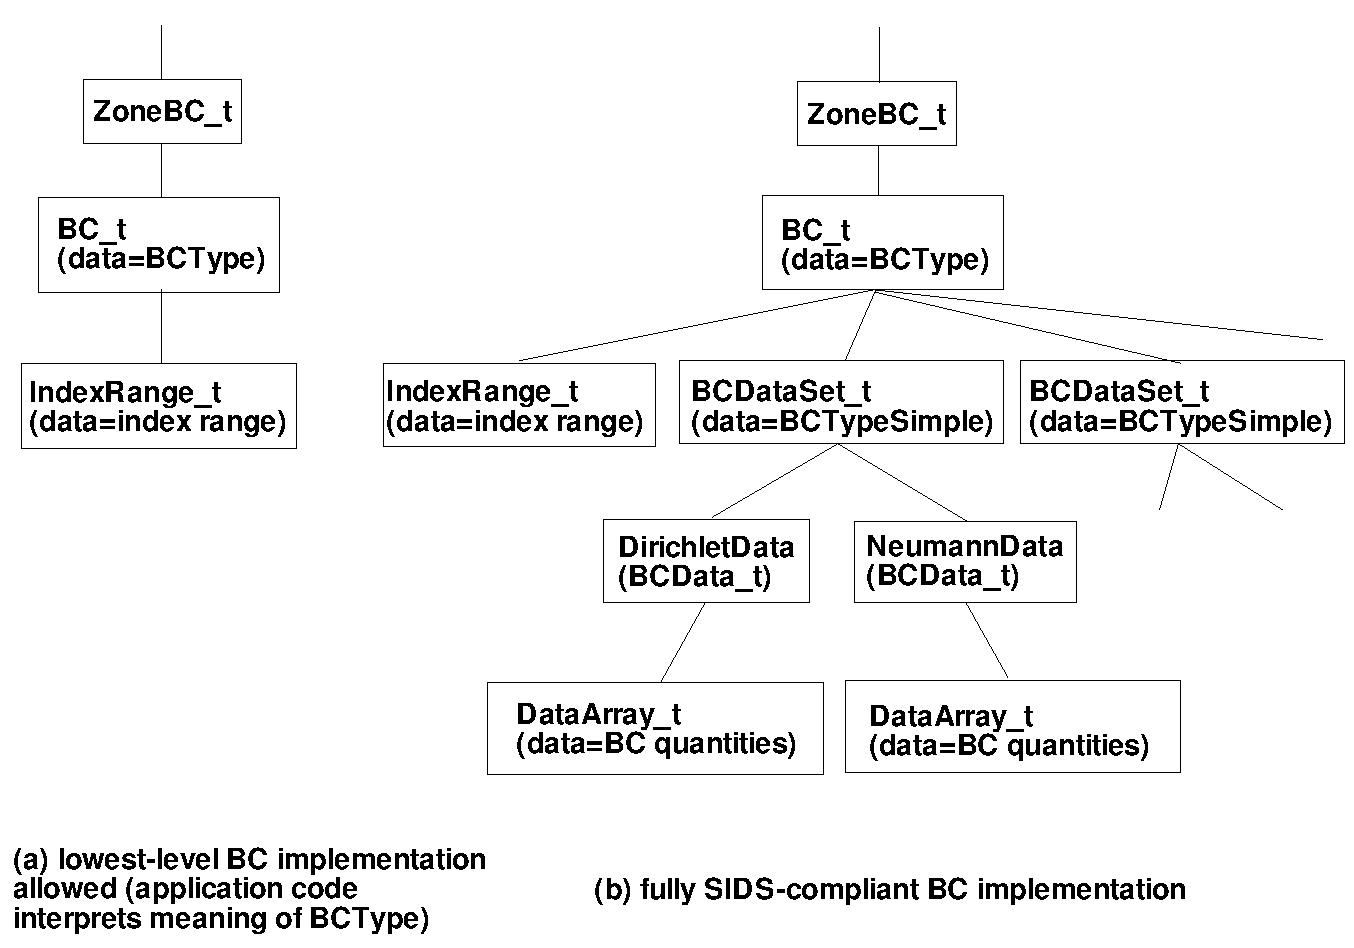
\includegraphics[width=150mm]{figures/bc}}}
\caption{General hierarchical structure of {\tt ZoneBC\_t}.}
\label{FIGbc}
\end{figure}
%

Example hierarchical structures for both the simplest 
implementation as well as the full-blown implementation
of the {\tt ZoneBC\_t} node are shown in Fig.~\ref{FIGbc}.  (These
hierarchies make use of an {\tt IndexRange\_t} node.  It is
also possible to use an {\tt IndexArray\_t}, which
gives a complete list of boundary indices or elements, rather than a
range.)  Note that an intermediate structure, where {\tt BCDataSet\_t} and
{\tt BCTypeSimple\_t} are both given but {\tt DirichletData} and
{\tt NeumannData} are not, is also allowed.
%In this case, the
%application code must interpret the combination of BCType\_t
%and whatever BCTypeSimple\_t's are given.

Many boundary condition types are currently defined in the SIDS,
but they by no means cover all possible boundary conditions.
The type {\tt UserDefinedData\_t} can be used for any special type not covered
that the user finds impossible to describe using the existing
SIDS.  When {\tt UserDefinedData\_t} is used,
a companion descriptor node is helpful to describe what was done.

~

%\renewcommand{\thesubsection}{}
%\subsection{\bf C.4  Zone Connectivity}
\subapp{Zone Connectivity}

It is often desirable to specify zone connectivity information when
parts of a zone connect with parts of another zone or itself.  The
connectivity information tells how zones fit together or how a
zone twists to reconnect with itself; the information
is needed by most CFD flow solvers.

There are three types of connectivity that can occur:  point-by-point,
patched, and overset.  The point-by-point, or 1-to-1, type occurs
when the edges of zones abut, and grid vertices from one patch
exactly correspond with grid vertices from the other, with no
points missing a partner.  The patched type occurs when
the edges of zones abut, but there is not a correspondence of the
points, or they are not partnered with another point.  The 
overset type occurs when zones overlap one another (or a zone overlaps
itself).

The SIDS allows for the specification of each of these types of zone 
connectivity under the {\tt ZoneGridConnectivity\_t} node.  All three
types can be implemented through the general {\tt GridConnectivity\_t} 
subnode (overset also requires the use of {\tt OversetHoles\_t} nodes).
However, the 1-to-1 type can also utilize, in certain
circumstances, the more specific {\tt GridConnectivity1to1\_t} subnode.

Fig.~\ref{FIGconnectivity} shows a sample hierarchy starting at the
{\tt ZoneGridConnectivity\_t} node, for a 1-to-1 type of interface
using a {\tt GridConnectivity1to1\_t} subnode.  Note in this figure that
we now list the name, label, and data within each node.  For this
structure, the naming convention at the bottom level
is particularly important, and
is actually more descriptive than the labels.  In fact, the label
for the {\tt Transform} node is very strange, and does not even follow 
the usual ``\_t'' convention.
As can be seen in the figure, multiple nodes are allowed under
the {\tt ZoneGridConnectivity\_t} node.  These can be any combination of
{\tt GridConnectivity1to1\_t}, {\tt GridConnectivity\_t}, 
{\tt OversetHoles\_t}, or {\tt Descriptor\_t} nodes.

% Figure
\begin{figure}[hpbt]
\centerline{{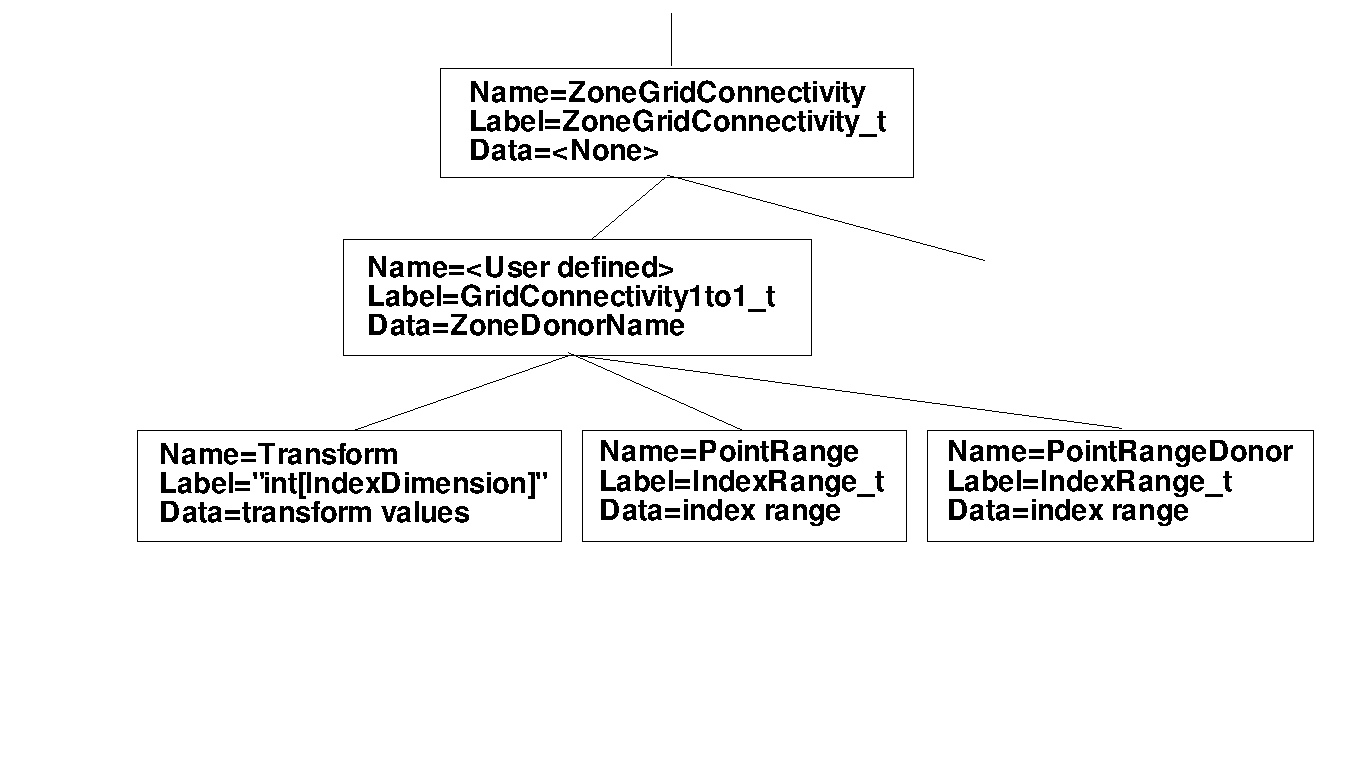
\includegraphics[width=150mm]{figures/connectivity}}}
\caption{Hierarchical structure of {\tt ZoneGridConnectivity\_t} for a
1-to-1 interface.}
\label{FIGconnectivity}
\end{figure}
%

A sample hierarchy (again starting at the {\tt ZoneGridConnectivity\_t} node)
is shown in Fig.~\ref{FIGconnectivityU} 
for an {\it overset} interface using a {\tt GridConnectivity\_t} 
subnode.  The case for a {\it patched} interface would look the
same, except there would be no {\tt OversetHoles\_t} node
or its children and {\tt GridConnectivityType} would be {\tt Abutting}.  Note that {\tt CellListDonor} 
and {\tt InterpolantsDonor} are used for
patched or overset interfaces.  ({\tt PointListDonor} can be 
used in their place if the interface is 1-to-1.)
See \cite{ALLMARAS} \cite{CGNS2} for details.)

% Figure
\begin{figure}[hpbt]
\centerline{{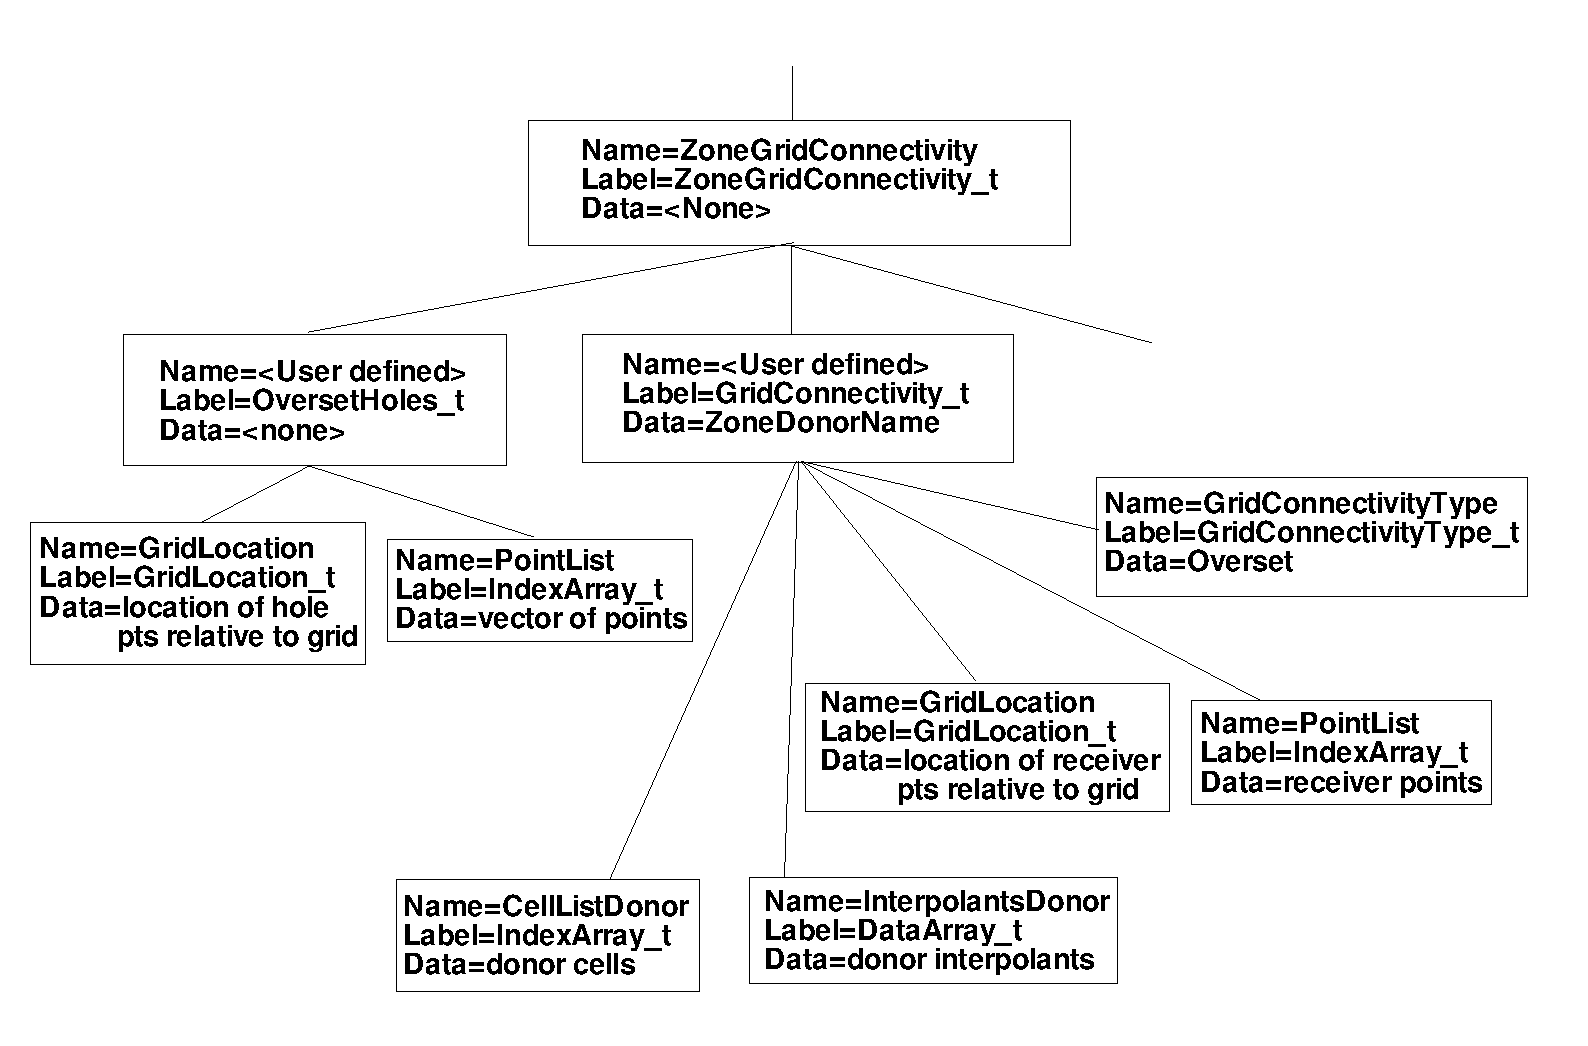
\includegraphics[width=150mm]{figures/connectivityU}}}
\caption{Hierarchical structure of {\tt ZoneGridConnectivity\_t} for an
overset interface.}
\label{FIGconnectivityU}
\end{figure}
%

~
\newpage
%\renewcommand{\thesubsection}{}
%\subsection{\bf C.5  Structured Zone Example}
\subapp{Structured Zone Example}

The following is an example for a structured grid.
It corresponds with example 8-A in the SIDS document \cite{ALLMARAS}.
It is a 3-D two-zone case, where the two zones are connected in
a 1-to-1 fashion at one of each of their faces.  Zone 1 is
$9 \times 17 \times 11$ and zone 2 is $9 \times 17 \times 21$.
The $k$-max face of zone 1 abuts the $k$-min face of zone 2.

The hierarchy
is shown in Figs.~\ref{FIGstr_exampleA} through \ref{FIGstr_exampleD}.  
Only directly relevant parts of the
hierarchy are shown here for clarity.  For example, {\tt DataClass\_t},
{\tt ReferenceState\_t}, {\tt ConvergenceHistory\_t}, 
{\tt FlowEquationSet\_t}, and {\tt ZoneBC\_t} 
have all been left off.  However, these (and other) items are
{\it not} required, and the figure still represents a valid
SIDS-compliant CGNS file.
Note that a data type of MT
indicates that there is no data stored in the node.

% Figure
\begin{figure}[hpbt]
\centerline{{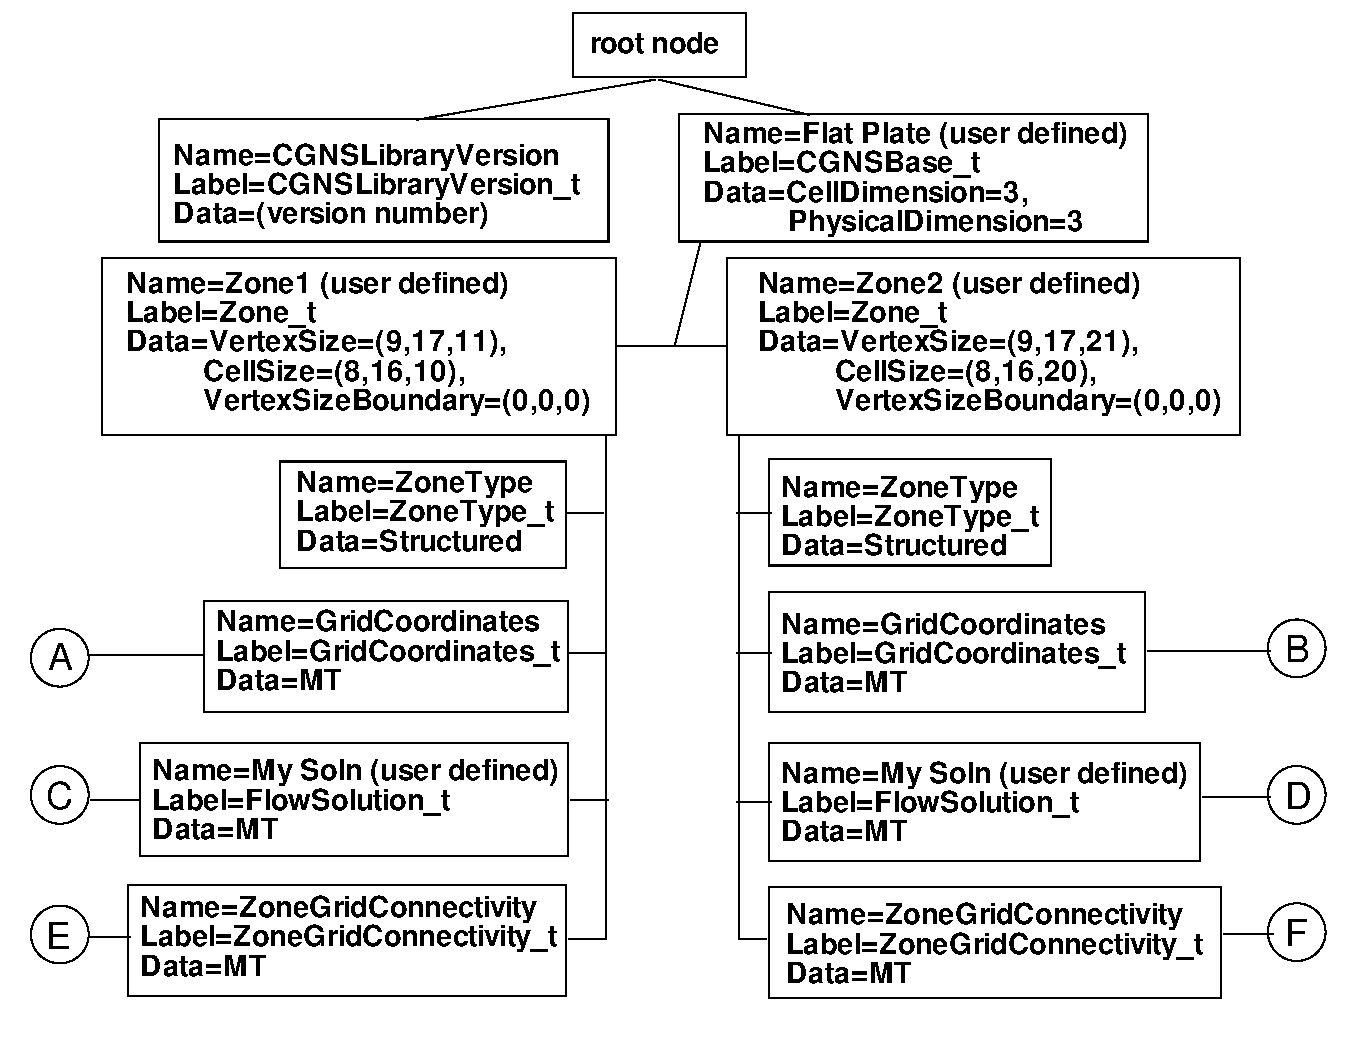
\includegraphics[width=150mm]{figures/str_exampleA}}}
\caption{CGNS top levels for a case composed of 2 structured zones.}
\label{FIGstr_exampleA}
\end{figure}
%
% Figure
\begin{figure}[hpbt]
\centerline{{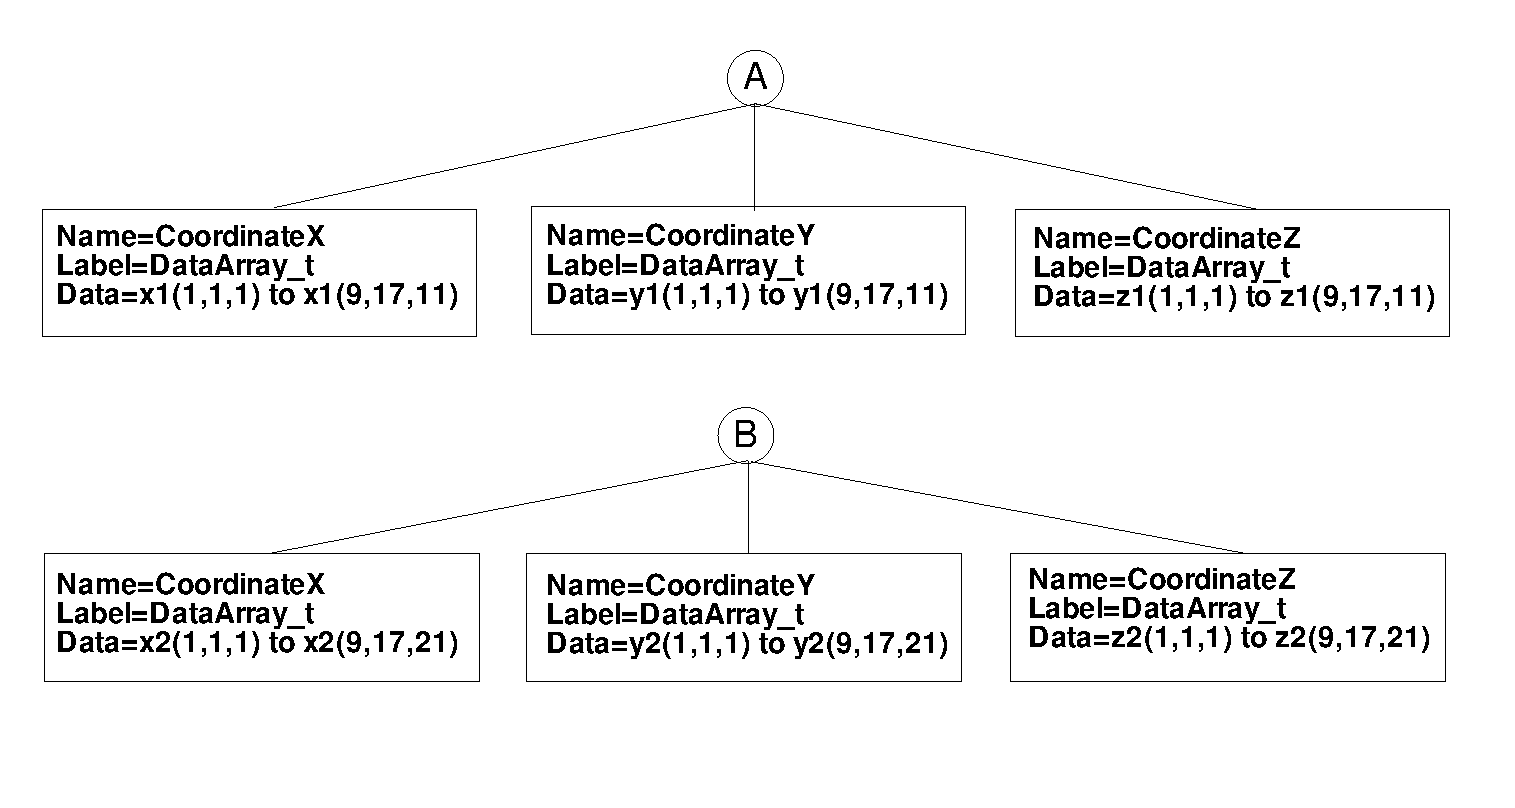
\includegraphics[width=150mm]{figures/str_exampleB}}}
\caption{{\tt GridCoordinate\_t} nodes of structured zone example.}
\label{FIGstr_exampleB}
\end{figure}
%
% Figure
\begin{figure}[hpbt]
\centerline{{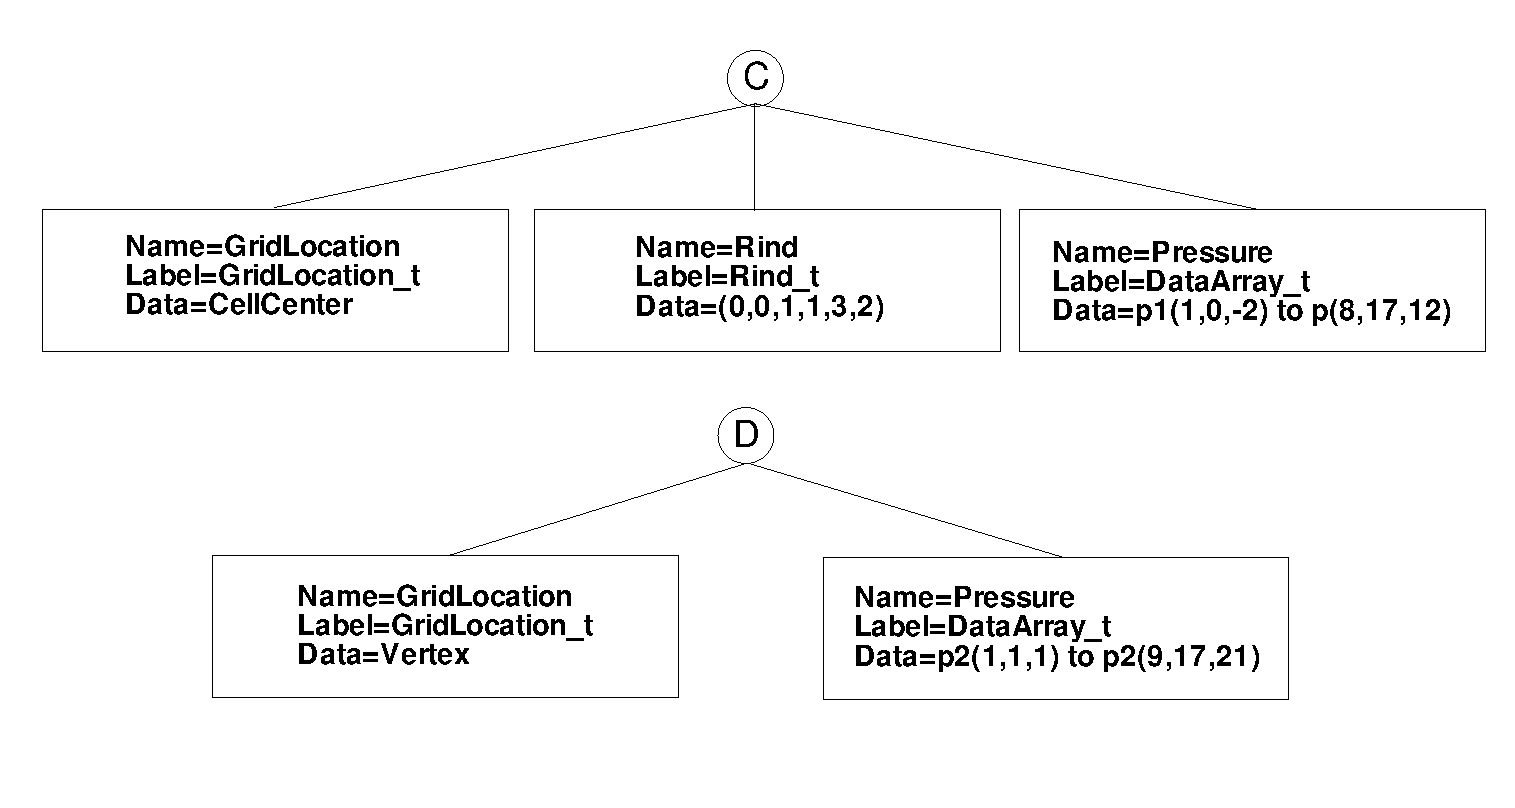
\includegraphics[width=150mm]{figures/str_exampleC}}}
\caption{{\tt FlowSolution\_t} nodes of structured zone example.}
\label{FIGstr_exampleC}
\end{figure}
%
% Figure
\begin{figure}[hpbt]
\centerline{{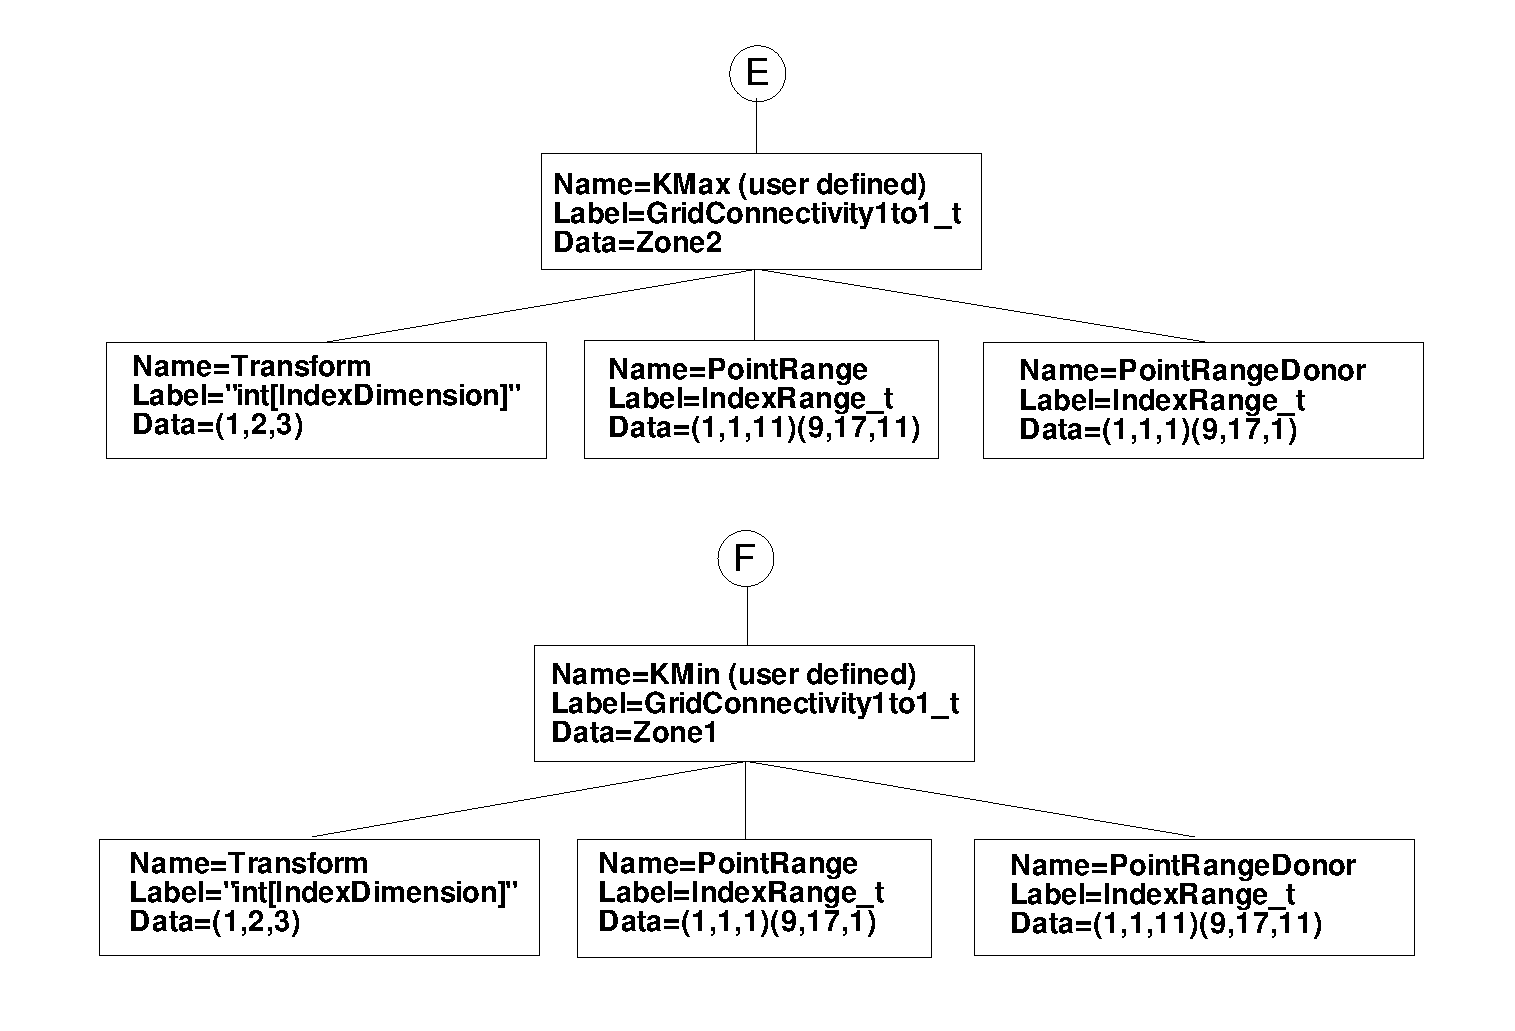
\includegraphics[width=150mm]{figures/str_exampleD}}}
\caption{{\tt ZoneGridConnectivity\_t} nodes of structured zone example.}
\label{FIGstr_exampleD}
\end{figure}
%

In this example, the flow solution in zone 1 is given at cell
centers, whereas the flow solution in zone 2 is given at the
vertices (see Fig.~\ref{FIGstr_exampleC}).  
In other words, the zone 1 solution points {\it do not}
correspond with the grid points (as they do in zone 2).  
They are defined {\it within} the volumes surrounded by the
grid points.  This example is constructed this way for the
purpose of illustration, but it is unusual; typically one would use 
only a single flow solution data location
for the entire file.
%This means that (if no Rind\_t were present)
%the flow solution for zone 1 would only exist over the 
%range $i$=1,8; $j$=1,16; and $k$=1,10.

This example also illustrates the use of the {\tt Rind\_t} node, and how
it affects the data arrays under a {\tt FlowSolution\_t}.  A rind
node under {\tt FlowSolution\_t} is used to indicate that the flow solution is outputting
additional rind or ``ghost'' data outside one or more boundaries
of the zone.  (A rind node can also be used under {\tt GridCoordinates\_t}
and {\tt DiscreteData\_t}.)
See the SIDS document \cite{ALLMARAS} for a more
complete description.  In zone 1 in this example, 
there are no additional ghost cell
data in the $i$-direction, there is one ghost cell next to
each of $j$-min and $j$-max, and there are 3 ghost cells next
to $k$-min and 2 next to $k$-max.  (Admittedly, this example is
very contrived - most applications would be more consistent
in their use of rind cells.)
Because of the rind cells, the $i$, $j$, and $k$ ranges of
all flow solution data arrays in zone 1 are extended appropriately.

It is very important for the user to realize that including rind 
cells affects how the data is stored in the {\tt DataArray\_t}'s.
In other words, when reading a CGNS file one cannot ignore
{\tt Rind\_t} nodes if they are present, and attempting to read
the {\tt DataArray\_t}'s using unmodified {\tt VertexSize} or 
{\tt CellSize} dimensions
will result in the retrieval of nonsensical data.

Note that the SIDS specifies many defaults.  For example, the
default {\tt Transform} values are (1,2,3), and the default
{\tt GridLocation} is {\tt Vertex}.  
Hence, the nodes that contain these particular
values in the example are not strictly necessary.
The API sometimes leaves out default information.

Another important fact is illustrated in this example.  When the names
of a type of node (of given label) are user defined, 
the names must be {\it different} if they
have the same parent node.  For example,
the two {\tt Zone\_t} nodes in this example must have different
names (recall the earlier discussion of zone naming).
However, if they are located in different places in the hierarchy, two
nodes with the same label can have the same name.  For example, 
both of the {\tt FlowSolution\_t} nodes, located in two different
zones, have been given the same user-defined
name:  ``{\tt My Soln}'' in the example.

Finally, although the {\tt ZoneBC\_t} nodes were not included in this
example, note that if they were, they should describe the boundary
conditions on all boundary faces {\it except} the 
$k$-max face of zone 1 and the $k$-min face of zone 2.  These
two faces would not be included in the boundary conditions because they
are already defined as connectivity interfaces.


\newpage
%\appendix
%\renewcommand{\thesection}{}
%\section{\bf APPENDIX D:  GUIDELINE FOR PLOT3D VARIABLES}
\app{GUIDELINE FOR PLOT3D \mbox{VARIABLES}}  \label{sec:plot3d}

The broad scope of CGNS allows users to essentially
put {\it anything} into a CGNS file.  While this is useful from the
perspective of extensibility, it also makes it more difficult
to read someone else's CGNS file without an elaborate
array of checks and translators.  This is true
not only because of the many choices of variables to output, but also
because CGNS allows many forms of dimensional and nondimensional
data.

Many people in the CFD community currently output structured-grids and
corresponding flow field data in PLOT3D
format \cite{WALATKA}, particularly for use in postprocessing visualization
programs.  It has, in some sense, become a {\it de facto} standard for
sharing structured CFD data.  Because this format is so widely used, we give
a guideline in this appendix for outputting and reading this type
of data in a CGNS file.  If you follow this guideline, then it is more likely
that other users will be able to easily read and interpret your
CGNS files.  

The PLOT3D standard grid variables are (in 3-D) $x$, $y$, and $z$.  These
coordinates may be dimensional or nondimensional.  To follow this
guideline, the three coordinates {\tt CoordinateX}, {\tt CoordinateY}, and
{\tt CoordinateZ} (either dimensional
or nondimensional) must be given.  There also may be
``iblank'' information, associated with overset grids.  
If used, the list of overset holes
is stored under {\tt OversetHoles\_t} nodes 
(see the SIDS document \cite{ALLMARAS}).  This appendix does not cover
the various dimensionalization and nondimensionalization
options for the grid coordinates.  By and large, from the point of view
of portability, the issue of units and/or nondimensionalization for
grid coordinates is not as crucial
as it is for the ``Q'' variables, which is covered in great detail below.
However, one should follow the SIDS standard and appropriately define
within the CGNS file the grid's units or nondimensionalizations used.

The PLOT3D standard ``Q'' variables are (in 3-D):

$\rho/\rho_{ref}$ = nondimensional density

$\rho u/(\rho_{ref}a_{ref})$ = nondimensional x-momentum

$\rho v/(\rho_{ref}a_{ref})$ = nondimensional y-momentum

$\rho w/(\rho_{ref}a_{ref})$ = nondimensional z-momentum

$\rho e_0/(\rho_{ref}a_{ref}^2)$ = nondimensional total energy per unit volume

\noindent where $a$ is the speed of sound and {\it ref} indicates
a reference state.  Standard PLOT3D Q files also
specify a reference Mach number, Reynolds number, angle of attack, and
time value.  For the purposes of this discussion, the time value will
not be addressed.
CGNS does have the capability for storing time-accurate data if
needed (see section~\ref{sec:timeacc}), but time-accurate data
is not covered in this PLOT3D guideline.
We include below the CGNS convention for
storing Mach number, Reynolds number, and (indirectly) angle of attack.

Each of the 5 flow field variables above has a standard name, defined in the SIDS.  They
are, respectively:  {\tt Density}, {\tt MomentumX}, {\tt MomentumY},
{\tt MomentumZ}, and {\tt EnergyStagnationDensity}.  To follow this
guideline, these are the 5 variables that should be output to your
CGNS file (in 3-D), and are also the ones that you should expect to read,
given someone else's CGNS file, if they are following this guideline.

Multiple bases are allowed in CGNS, but, to further enhance
portability of PLOT3D-like datasets, only one {\tt CGNSBase\_t} node is 
recommended under this guideline.  In other words, multiple cases
(such as different angles of attack) should be stored in separate
CGNS files with single bases, rather than in a single file with multiple bases.

The three most common types of data that one may output in a CGNS file are:

{\tt DataClass = Dimensional}

{\tt DataClass = NormalizedByDimensional}

{\tt DataClass = NormalizedByUnknownDimensional}

The first category indicates that the data has dimensional units.
The second category indicates that
the data has been nondimensionalized by {\it known} reference
values, which are specified in the CGNS file.  
The third category indicates that the data is nondimensional,
but the reference values are
unspecified or unknown.  Because CGNS deals with each of these in a 
slightly different way, we will give the guideline for each of
these three classes in separate subsections.

%\renewcommand{\thesubsection}{}
%\subsection{\bf D.1  Dimensional Data} \label{sec:dimdata}
\subapp{Dimensional Data} \label{sec:dimdata}

To output dimensional data:

\begin{enumerate}
\item Under {\tt CGNSBase\_t}, set {\tt DataClass = Dimensional}.

\item Under {\tt CGNSBase\_t}, put a {\tt ReferenceState}; and under
{\tt ReferenceState}, put the dimensional reference
values of {\tt Density} and {\tt VelocitySound}.
Under this guideline, the units of these
must be consistent with one another and with the units
of {\tt Density}, {\tt MomentumX}, {\tt MomentumY},
{\tt MomentumZ}, and {\tt EnergyStagnationDensity} given
under {\tt FlowSolution} (e.g., all MKS units).
Also under {\tt ReferenceState},
put {\tt Mach}, {\tt Reynolds},
{\tt VelocityX}, {\tt VelocityY}, and {\tt VelocityZ}.  

\item Under {\tt FlowSolution}, put the dimensional variables
{\tt Density}, {\tt MomentumX}, {\tt MomentumY},
{\tt MomentumZ}, and {\tt EnergyStagnationDensity}.
Under this guideline, the units of these 5 variables
must be consistent with one another and with the
units of {\tt Density} and {\tt VelocitySound} in 
{\tt ReferenceState}.

\end{enumerate}

\noindent To read dimensional data (i.e., if {\tt DataClass = Dimensional}
under {\tt CGNSBase\_t}):

\begin{enumerate}

\item Under {\tt ReferenceState} (directly under {\tt CGNSBase\_t}),
read {\tt Density}, {\tt VelocitySound},
{\tt Mach}, and {\tt Reynolds}.
Also read {\tt VelocityX}, {\tt VelocityY}, and {\tt VelocityZ}
if an angle of attack of the reference state is needed.

\item Under {\tt FlowSolution}, read
{\tt Density}, {\tt MomentumX}, {\tt MomentumY},
{\tt MomentumZ}, and 
\newline {\tt EnergyStagnationDensity}.

\item To obtain the PLOT3D Q variables, do the following:

$\rho/\rho_{ref}$ = {\tt Density} / {\tt Density(ref)}

$\rho u/(\rho_{ref}a_{ref})$ = {\tt MomentumX} / ({\tt Density(ref)} * {\tt VelocitySound(ref)})

$\rho v/(\rho_{ref}a_{ref})$ = {\tt MomentumY} / ({\tt Density(ref)} * {\tt VelocitySound(ref)})

$\rho w/(\rho_{ref}a_{ref})$ = {\tt MomentumZ} / ({\tt Density(ref)} * {\tt VelocitySound(ref)})

$\rho e_0/(\rho_{ref}a_{ref}^2)$ = {\tt EnergyStagnationDensity} /
({\tt Density(ref)} * {\tt VelocitySound(ref)}$^2$)

\end{enumerate}


%\renewcommand{\thesubsection}{}
%\subsection{\bf D.2  NormalizedByDimensional Data} \label{sec:normdimdata}
\subapp{NormalizedByDimensional Data} \label{sec:normdimdata}

To output nondimensional data with known normalizations:

\begin{enumerate}
\item Under {\tt CGNSBase\_t}, set {\tt DataClass = NormalizedByDimensional}.

\item Under {\tt CGNSBase\_t}, put a {\tt ReferenceState}; and under
{\tt ReferenceState}, put {\tt Mach}, {\tt Reynolds},
{\tt VelocityX}, {\tt VelocityY}, and {\tt VelocityZ}.  Then put either:

\begin{itemize}
\item The {\it dimensional} reference
values of {\tt Density} and {\tt VelocitySound}.
Under this guideline, the units of these
must be consistent with one another and with the units of the {\it raw} (dimensional) data
{\tt Density}, {\tt MomentumX}, {\tt MomentumY},
{\tt MomentumZ}, and {\tt EnergyStagnationDensity} given
under {\tt FlowSolution}, prior to normalization.

\item The {\it nondimensional} reference
values of {\tt Density} and {\tt VelocitySound}, along with
their corresponding {\tt ConversionScale} and {\tt ConversionOffset}
values.
Under this guideline, the units of the {\it raw} (dimensional) 
{\tt Density} and {\tt VelocitySound},
prior to normalization using {\tt ConversionScale} and {\tt ConversionOffset},
must be consistent with one another and with the 
units of the {\it raw} (dimensional) data
{\tt Density}, {\tt MomentumX}, {\tt MomentumY},
{\tt MomentumZ}, and {\tt EnergyStagnationDensity} given
under {\tt FlowSolution}, prior to normalization.

\end{itemize}
 
\item Under {\tt FlowSolution}, put the nondimensional variables
{\tt Density}, {\tt MomentumX}, {\tt MomentumY},
{\tt MomentumZ}, and {\tt EnergyStagnationDensity}, along with
their corresponding {\tt ConversionScale} and {\tt ConversionOffset}
values.
Under this guideline, the units of the {\it raw} (dimensional)
variables, prior to normalization using {\tt ConversionScale} and {\tt ConversionOffset},
must be consistent with one another and with the
units of the {\it raw} (dimensional) {\tt Density} and {\tt VelocitySound}
in {\tt ReferenceState}.

\end{enumerate}

\noindent To read nondimensional data with known normalizations 
(i.e., if {\tt DataClass =} 
\newline {\tt NormalizedByDimensional}
under {\tt CGNSBase\_t}):

\begin{enumerate}

\item Under {\tt ReferenceState} (directly under {\tt CGNSBase\_t}),
read {\tt Density} and {\tt VelocitySound}.  Also read their 
{\tt ConversionScale} and {\tt ConversionOffset} values if they are present.
Additionally, read {\tt Mach} and {\tt Reynolds}.
Also read {\tt VelocityX}, {\tt VelocityY}, and {\tt VelocityZ}
if an angle of attack of the reference state is needed.

\item Under {\tt FlowSolution}, read
{\tt Density}, {\tt MomentumX}, {\tt MomentumY},
{\tt MomentumZ}, and 
\newline {\tt EnergyStagnationDensity}.
Also read each {\tt ConversionScale} and {\tt ConversionOffset}.

\item To obtain the
PLOT3D Q variables, do the following.  First, {\it only if they were
given as nondimensional quantities} (indicated by a {\tt '} below), 
recover the {\it raw} (dimensional) reference
values of {\tt Density} and {\tt VelocitySound}, via:

{\tt Density(ref)} = {\tt Density'(ref)}*{\tt ConversionScale} + {\tt ConversionOffset}

{\tt VelocitySound(ref)} = {\tt VelocitySound'(ref)}*{\tt ConversionScale} + {\tt ConversionOffset}

\noindent Then do:

$\rho/\rho_{ref}$ = ({\tt Density}*{\tt ConversionScale} + {\tt ConversionOffset}) 
/ {\tt Density(ref)}

$\rho u/(\rho_{ref}a_{ref})$ = ({\tt MomentumX}*{\tt ConversionScale} + {\tt ConversionOffset})  
/ ({\tt Density(ref)} * {\tt VelocitySound(ref)})

$\rho v/(\rho_{ref}a_{ref})$ = ({\tt MomentumY}*{\tt ConversionScale} + {\tt ConversionOffset}) 
/ ({\tt Density(ref)} * {\tt VelocitySound(ref)})

$\rho w/(\rho_{ref}a_{ref})$ = ({\tt MomentumZ}*{\tt ConversionScale} + {\tt ConversionOffset}) 
/ ({\tt Density(ref)} * {\tt VelocitySound(ref)})

$\rho e_0/(\rho_{ref}a_{ref}^2)$ = ({\tt EnergyStagnationDensity}*{\tt ConversionScale} + 
{\tt ConversionOffset}) /
({\tt Density(ref)} * {\tt VelocitySound(ref)}$^2$)

\end{enumerate}

Note that it is possible that the conversion scale and offset for the PLOT3D Q variables
may correspond to the reference conditions.  This would imply that the variables could
be directly output, without the above conversions needed.  However, CGNS allows the
variables to be normalized by properties independent of the reference conditions, so
the above procedure is recommended to avoid ambiguity.


%\renewcommand{\thesubsection}{}
%\subsection{\bf D.3  NormalizedByUnknownDimensional Data} \label{sec:nondimdata}
\subapp{NormalizedByUnknownDimensional Data} \label{sec:nondimdata}

To output nondimensional data with unknown normalizations:

\begin{enumerate}
\item Under {\tt CGNSBase\_t}, set {\tt DataClass = NormalizedByUnknownDimensional}.

\item Under {\tt CGNSBase\_t}, put a {\tt ReferenceState}; and under
{\tt ReferenceState}, put 
{\tt Density} = 1 and {\tt VelocitySound} = 1.
Also, put {\tt Mach}, {\tt Reynolds},
{\tt VelocityX}, {\tt VelocityY}, and {\tt VelocityZ}. 

\item Under {\tt FlowSolution}, put the nondimensional variables
{\tt Density}, {\tt MomentumX}, {\tt MomentumY},
{\tt MomentumZ}, and {\tt EnergyStagnationDensity}. 
These must be nondimensionalized as:
$\rho/\rho_{ref}$,
$\rho u/(\rho_{ref}a_{ref})$,
$\rho v/(\rho_{ref}a_{ref})$,
$\rho w/(\rho_{ref}a_{ref})$,
$\rho e_0/(\rho_{ref}a_{ref}^2)$.

\end{enumerate}

\noindent (Setting {\tt Density} = 1 and {\tt VelocitySound} = 1 in the
{\tt ReferenceState} defines the particular nondimensionalization
defined above for the PLOT3D variables; see the SIDS document \cite{ALLMARAS}
for details and other examples.)
To read nondimensional data with unknown normalizations
(i.e., if {\tt DataClass =} 
{\tt NormalizedByUnknownDimensional}
under {\tt CGNSBase\_t}):

\begin{enumerate}
\item Check under {\tt ReferenceState} (directly under {\tt CGNSBase\_t}),
to be sure that {\tt Density} = 1 and {\tt VelocitySound} = 1.
Then, read {\tt Mach} and {\tt Reynolds}.
Also read {\tt VelocityX}, {\tt VelocityY}, and {\tt VelocityZ}
if an angle of attack of the reference state is needed.

\item Under {\tt FlowSolution}, read
{\tt Density}, {\tt MomentumX}, {\tt MomentumY},
{\tt MomentumZ}, and 
\newline {\tt EnergyStagnationDensity}.

\end{enumerate}

Nothing needs to be done in this case
to obtain the PLOT3D Q variables.  They are already in
the correct form.

%\renewcommand{\thesubsection}{}
%\subsection{\bf D.4  Notes} \label{sec:notesD}
\subapp{Notes} \label{sec:notesD}

\begin{enumerate}
\item In addition to the flow field variables
{\tt Density}, {\tt MomentumX}, {\tt MomentumY},
{\tt MomentumZ}, and {\tt EnergyStagnationDensity} (under {\tt FlowSolution}), you may
also output additional variables if desired, 
but be sure these 5 are present. \label{Itemnote1}

\item Other reference values may also be placed under
{\tt ReferenceState} (for example, {\tt LengthReference} may be needed to define
the reference length associated with the grid coordinates), 
but the use of {\tt Density} and {\tt VelocitySound}
is sufficient to define the nondimensionalizations of the PLOT3D Q
variables.  \label{Itemnote2}

\item The quantities {\tt Mach}, {\tt Reynolds},
{\tt VelocityX}, {\tt VelocityY}, {\tt VelocityZ},
{\tt Density}, and {\tt VelocitySound} (plus anything else)
under {\tt ReferenceState}
must all represent the same reference state of the
flow.  For external aerodynamics, this is usually taken to be
the free stream, but it does not have to be. \label{Itemnote3}

\item The velocity components are used, in the PLOT3D sense, solely to
provide an angle of attack of the flow field at the reference
state.  The definition of angle of attack itself is non-unique in 3-D, so there
is therefore no SIDS standard for it.  For example, one
possible set of angle definitions assumes that the $z$-direction is ``up,''
and uses:

$u = V{\rm cos}\beta {\rm cos}\alpha$

$v = -V{\rm sin} \beta$

$w = V{\rm cos}\beta{\rm sin}\alpha$ 

\noindent where $V=\sqrt{u^2+v^2+w^2}$, $\alpha$ is angle of attack,
and $\beta$ is angle of sideslip.  Thus, an angle of attack 
can be obtained using $\alpha = {\rm tan}^{-1}(w/u)$, where $u$ = {\tt VelocityX}
and $w$ = {\tt VelocityZ}.  \label{Itemnote4}

\item When reading someone else's CGNS file, a low-level
approach to interpret and/or use it
appropriately would be the following.  First, check to see that there
is only one {\tt CGNSBase\_t} node.  (As discussed above, multiple bases
are allowed in general, but under this guideline only one base should exist.)
Second, insure that the variables {\tt CoordinateX}, {\tt CoordinateY},
and {\tt CoordinateZ} exist under each zone's {\tt GridCoordinates\_t} node,
and that the variables {\tt Density}, {\tt MomentumX}, {\tt MomentumY},
{\tt MomentumZ}, and {\tt EnergyStagnationDensity} exist under each 
zone's {\tt FlowSolution\_t} node.  (Note:  for time-accurate datasets
there may be multiple {\tt GridCoordinates\_t} and 
{\tt FlowSolution\_t} nodes under each 
zone -- see section~\ref{sec:timeacc} -- but this situation is not
covered under the current PLOT3D guideline.)  Then, search for the following 
characteristics in the file:

\begin{itemize}
\item If {\tt DataClass = Dimensional}, then {\tt ReferenceState}
(directly under {\tt CGNSBase\_t}) {\it must} contain {\tt Density},
{\tt VelocitySound}, {\tt Mach}, and {\tt Reynolds}.  {\tt VelocityX},
{\tt VelocityY}, and {\tt VelocityZ} are needed under {\tt ReferenceState} only if a reference
angle of attack is required.

\item If {\tt DataClass = NormalizedByDimensional}, then {\tt ReferenceState}
(directly under {\tt CGNSBase\_t}) {\it must} contain {\tt Density},
{\tt VelocitySound}, {\tt Mach}, and {\tt Reynolds}.  {\tt VelocityX},
{\tt VelocityY}, and {\tt VelocityZ} are needed under {\tt ReferenceState} only if a reference
angle of attack is required.  Furthermore, a
{\tt ConversionScale} and {\tt ConversionOffset}
must exist for each of the 5 flow field variables
under {\tt FlowSolution}.  {\tt ConversionScale} and {\tt ConversionOffset}
may or may not exist for the variables under {\tt ReferenceState}.

\item If {\tt DataClass = NormalizedByUnknownDimensional},
then {\tt ReferenceState} (directly under {\tt CGNSBase\_t}) {\it must}
contain {\tt Density} = 1, {\tt VelocitySound} = 1, as well as
{\tt Mach}, and {\tt Reynolds}.  {\tt VelocityX},
{\tt VelocityY}, and {\tt VelocityZ} are needed under {\tt ReferenceState} only if a reference
angle of attack is required.

\end{itemize}

\noindent If these conditions are met, then a low-level
reader could assume that the guidelines outlined in the above 
subsections were
followed, and the PLOT3D variables could easily be obtained
using the procedures given.  A more advanced reader would
probably check for consistency in the dimensions and conversion
scales, to ensure compliance with the guidelines.  \label{Itemnote5}

\end{enumerate}

\begin{thebibliography}{99}

%%%
\bibitem{ALLMARAS}
CGNS Project Group,
``The CFD General Notation System Standard Interface Data Structures,''
Version 2.0 beta 2, February 2001;
http://www.grc.nasa.gov/www/cgns/sids/index.html
%%%

%%%
\bibitem{CGNS1}
CGNS Project Group,
``The CFD General Notation System Advanced Data Format (ADF) User's Guide,''
April 2001;
http://www.grc.nasa.gov/www/cgns/adf/index.html
%%%

%%%
\bibitem{CGNS2}
CGNS Project Group,
``The CFD General Notation System SIDS-to-ADF File Mapping Manual,''
Version 1.2 revision 8, February 2001;
http://www.grc.nasa.gov/www/cgns/filemap/index.html
%%%

%%%
\bibitem{POIRIER98}
Poirier, D. M. A., Allmaras, S., McCarthy, D. R., Smith, M., and
Enomoto, F.,
``The CGNS System,''
AIAA Paper 98-3007, June 1998.
%%%

%%%
\bibitem{POIRIER99}
CGNS Project Group,
``The CFD General Notation System Mid-Level Library,''
July 2001;
http://www.grc.nasa.gov/www/cgns/midlevel/index.html
%%%

%%%
\bibitem{POIRIER00}
Poirier, D. M. A., Bush, R. H., Cosner, R. R., Rumsey, C. L., and
McCarthy, D. R.,
``Advances in the CGNS Database Standard for Aerodynamics and CFD,''
AIAA Paper 2000-0681, January 2000.
%%%

%%%
\bibitem{WALATKA}
Walatka, P. P., Buning, P. G., Pierce, L., Elson, P. A.,
``PLOT3D User's Guide,''
NASA TM 101067, March 1990.
%%%

\end{thebibliography}
%

\end{document}

